%********************************************************************
% Title: Business Research Methods
% Description: An Open Educational Resource for my BASV 316 class
% Author: George Self
% History: 
%   170101: Started This Puppy
%	170715: Re-started my work on this
%   180601: Re-started (again)
%   190206: Finished the really rough draft
%   190609: First draft completed
%********************************************************************

\RequirePackage{fix-cm} % fix some latex issues see: http://texdoc.net/texmf-dist/doc/latex/base/fixltx2e.pdf
\documentclass[ twoside, openright, titlepage, numbers=noenddot, headinclude,
  %1headlines, % letterpaper a4paper, 
  footinclude=true, cleardoublepage=empty, abstractoff, 
  % <--- obsolete, remove (todo)
  BCOR=5mm, 
  %paper=a4,
  paper=letter, fontsize=11pt,
  % ngerman (New German) formats German umlauts (among other things)
  american
  %
]{scrreprt}

%*********************************************************************
% Note: Make all your adjustments in here
%*********************************************************************
% *************************************************
% classicthesis-config.tex 
% Use it at the beginning of your ClassicThesis.tex, or as a LaTeX Preamble 
% in your ClassicThesis.{tex,lyx} with \input{classicthesis-config}
% *************************************************

% *************************************************
% 0. Set the encoding of your files. UTF-8 is the only sensible encoding nowadays. If you can't read
% äöüßáéçèê∂åëæƒÏ€ then change the encoding setting in your editor, not the line below. If your editor
% does not support utf8 use another editor!
% *************************************************
\PassOptionsToPackage{utf8}{inputenc}
  \usepackage{inputenc}

% *************************************************
% 1. Configure classicthesis for your needs here, e.g., remove "drafting" below 
% in order to deactivate the time-stamp on the pages
% *************************************************
\PassOptionsToPackage{eulerchapternumbers,listings,drafting,%
  pdfspacing,%floatperchapter,%linedheaders,%
  subfig,beramono,eulermath,parts}{classicthesis}

% *************************************************
% Available options for classicthesis.sty 
% (see ClassicThesis.pdf for more information):
% drafting
% parts nochapters linedheaders
% eulerchapternumbers beramono eulermath pdfspacing minionprospacing
% tocaligned dottedtoc manychapters
% listings floatperchapter subfig
% *************************************************

% *************************************************
% 2. Personal data and user ad-hoc commands
% *************************************************
\newcommand{\myTitle}{Research Methods\xspace}
\newcommand{\mySubtitle}{For Business and Marketing\xspace}
\newcommand{\myDegree}{Masters of Science\xspace}
\newcommand{\myName}{George Self\xspace}
\newcommand{\myProf}{Put name here\xspace}
\newcommand{\myOtherProf}{Put name here\xspace}
\newcommand{\mySupervisor}{Put name here\xspace}
\newcommand{\myFaculty}{Put data here\xspace}
\newcommand{\myDepartment}{Put data here\xspace}
\newcommand{\myUni}{University of South Arizona\xspace}
\newcommand{\myLocation}{Sierra Vista, AZ\xspace}
\newcommand{\myTime}{January, 2019\xspace}
\newcommand{\myVersion}{Edition 1\xspace}

% *************************************************
% Setup, finetuning, and useful commands
% *************************************************
\newcounter{dummy} % necessary for correct hyperlinks (to index, bib, etc.)
\newlength{\abcd} % for ab..z string length calculation
\providecommand{\mLyX}{L\kern-.1667em\lower.25em\hbox{Y}\kern-.125emX\@}
\newcommand{\ie}{i.\,e.}
\newcommand{\Ie}{I.\,e.}
\newcommand{\eg}{e.\,g.}
\newcommand{\Eg}{E.\,g.}

% Create a blank page at the end of the document
\newcommand{\blankpage}{ 
	\newpage
	\thispagestyle{empty}
	\mbox{}
	\newpage
}

% The following creates a function named maxwidth that permits
% me to set a maximum width for images. If the natural width of
% the image is less than maxwidth then the image is rendered at
% its natural size, else scaled to maxwidth.
\makeatletter
\def\maxwidth#1{\ifdim\Gin@nat@width>#1 #1\else\Gin@nat@width\fi}
\makeatother

% *************************************************

% *************************************************
% My Packages
% *************************************************
\usepackage[
	type={CC},
	modifier={by-nc-sa},
	version={4.0}
]{doclicense} % Prints the Creative Commons license

\usepackage[obeyspaces,hyphens]{url}
\expandafter\def\expandafter\UrlBreaks\expandafter{\UrlBreaks%  save the current one
	\do\a\do\b\do\c\do\d\do\e\do\f\do\g\do\h\do\i\do\j%
	\do\k\do\l\do\m\do\n\do\o\do\p\do\q\do\r\do\s\do\t%
	\do\u\do\v\do\w\do\x\do\y\do\z\do\A\do\B\do\C\do\D%
	\do\E\do\F\do\G\do\H\do\I\do\J\do\K\do\L\do\M\do\N%
	\do\O\do\P\do\Q\do\R\do\S\do\T\do\U\do\V\do\W\do\X%
	\do\Y\do\Z}


% *************************************************

% *************************************************
% 3. Loading some handy packages
% *************************************************

% *************************************************
% Packages with options that might require adjustments
% *************************************************
%\PassOptionsToPackage{ngerman,american}{babel}   % change this to your language(s)
% Spanish languages need extra options in order to work with this template
%\PassOptionsToPackage{spanish,es-lcroman}{babel}
\usepackage{babel}

\usepackage{csquotes}

\PassOptionsToPackage{%
  backend=biber, %instead of bibtex
  backend=bibtex8,bibencoding=ascii,%
  language=auto,%
  style=numeric-comp,%
    %style=authoryear-comp, % Author 1999, 2010
    %bibstyle=authoryear,dashed=false, % dashed: substitute rep. author with ---
  sorting=nyt, % name, year, title
  maxbibnames=10, % default: 3, et al.
    %backref=true,%
  natbib=true % natbib compatibility mode (\citep and \citet still work)
  }{biblatex}
  \usepackage{biblatex}
\addbibresource{ResearchMethods}

% math environments and more by the AMS 
\PassOptionsToPackage{fleqn}{amsmath}  
  \usepackage{amsmath}

% *************************************************
% General useful packages
% *************************************************
\PassOptionsToPackage{T1}{fontenc} % T2A for cyrillics
  \usepackage{fontenc}     
\usepackage{textcomp} % fix warning with missing font shapes
\usepackage{scrhack} % fix warnings when using KOMA with listings package          
\usepackage{xspace} % to get the spacing after macros right  
\usepackage{mparhack} % get marginpar right
\usepackage{fixltx2e} % fixes some LaTeX stuff 

%\PassOptionsToPackage{printonlyused,smaller}{acronym} 
%  \usepackage{acronym} % nice macros for handling all acronyms in the thesis
%\renewcommand*{\aclabelfont}[1]{\acsfont{#1}}

\usepackage{shorttoc} % For the short TOC at the top of the document

% ***********************************************
% Used for wrapping figures
% ***********************************************
\usepackage{float}
\usepackage{wrapfig}
\restylefloat{figure}

% *************************************************
% 4. Setup tables, (sub)figures, and captions
% *************************************************
\usepackage[svgnames,table]{xcolor} % control row/cell color in a table
\usepackage{tabularx} % better tables
\usepackage{tabulary} % another tables option
\setlength{\extrarowheight}{3pt} % increase table row height
\newcommand{\tableheadline}[1]{\multicolumn{1}{c}{\spacedlowsmallcaps{#1}}}
\newcommand{\myfloatalign}{\centering} % to be used with each float for alignment
\usepackage{tikz} % for drawing
\usetikzlibrary{positioning}
\usetikzlibrary{arrows}

\usepackage{caption}
\captionsetup{font=small} % format=hang,
\usepackage{subfig}  

\usepackage{booktabs}
% *************************************************

% *************************************************
% Objectives boxes
% *************************************************
\usepackage{tcolorbox} % create nice color boxes
\definecolor{objgold}{RGB}{255,178,102}
\definecolor{tkawyblue}{RGB}{102,255,255}
\newtcolorbox{objbox}[1]{
	colback=objgold!5!white,
	colframe=objgold!85!black,
	fonttitle=\bfseries,
	width=.75\linewidth,
	title=#1}

\newtcolorbox{tkawybox}[1]{
	colback=tkawyblue!5!white,
	colframe=tkawyblue!70!black,
	fonttitle=\bfseries,
	width=.75\linewidth,
	title=#1}

% *************************************************
% 5. Setup code listings
% *************************************************
\usepackage{listings} 
\lstset{language=[LaTeX]Tex,%C++,
    morekeywords={PassOptionsToPackage,selectlanguage},
    keywordstyle=\color{RoyalBlue},%\bfseries,
    basicstyle=\small\ttfamily,
    %identifierstyle=\color{NavyBlue},
    commentstyle=\color{Green}\ttfamily,
    stringstyle=\rmfamily,
    numbers=none,%left,%
    numberstyle=\scriptsize,%\tiny
    stepnumber=5,
    numbersep=8pt,
    showstringspaces=false,
    breaklines=true,
    %frameround=ftff,
    %frame=single,
    belowcaptionskip=.75\baselineskip
    %frame=L
}
% *************************************************


% *************************************************
% Create a new command, blfootnote, that does not use 
% a footnote marker
% *************************************************
\newcommand\blfootnote[1]{%
	\begingroup
	\renewcommand\thefootnote{}\footnote{#1}%
	\addtocounter{footnote}{-1}%
	\endgroup
}

% *************************************************
% 6. PDFLaTeX, hyperreferences and citation backreferences
% *************************************************

% *************************************************
% Using PDFLaTeX
% *************************************************
\PassOptionsToPackage{pdftex,hyperfootnotes=false,pdfpagelabels}{hyperref}
  \usepackage{hyperref}  % backref linktocpage pagebackref
\pdfcompresslevel=9
\pdfadjustspacing=1 
\PassOptionsToPackage{pdftex}{graphicx}
  \usepackage{graphicx} 

% *************************************************
% Hyperreferences
% *************************************************
\hypersetup{%
  %draft, % = no hyperlinking at all (useful in b/w printouts)
  colorlinks=true, linktocpage=true, pdfstartpage=3, pdfstartview=FitV,%
  % uncomment the following line if you want to have black links (e.g., for printing)
  %colorlinks=false, linktocpage=false, pdfstartpage=3, pdfstartview=FitV, pdfborder={0 0 0},%
  breaklinks=true, pdfpagemode=UseNone, pageanchor=true, pdfpagemode=UseOutlines,%
  plainpages=false, bookmarksnumbered, bookmarksopen=true, bookmarksopenlevel=1,%
  hypertexnames=true, pdfhighlight=/O,%nesting=true,%frenchlinks,%
  urlcolor=webbrown, linkcolor=RoyalBlue, citecolor=webgreen, %pagecolor=RoyalBlue,%
  %urlcolor=Black, linkcolor=Black, citecolor=Black, %pagecolor=Black,%
  pdftitle={\myTitle},%
  pdfauthor={\textcopyright\ \myName, \myUni, \myFaculty},%
  pdfsubject={},%
  pdfkeywords={},%
  pdfcreator={pdfLaTeX},%
  pdfproducer={LaTeX with hyperref and classicthesis}%
}


% *************************************************
% Setup autoreferences
% *************************************************
% There are some issues regarding autorefnames
% http://www.ureader.de/msg/136221647.aspx
% http://www.tex.ac.uk/cgi-bin/texfaq2html?label=latexwords
% you have to redefine the makros for the 
% language you use, e.g., american, ngerman
% (as chosen when loading babel/AtBeginDocument)
% *************************************************
\makeatletter
\@ifpackageloaded{babel}%
  {%
    \addto\extrasamerican{%
    \renewcommand*{\figureautorefname}{Figure}%
    \renewcommand*{\tableautorefname}{Table}%
    \renewcommand*{\partautorefname}{Part}%
    \renewcommand*{\chapterautorefname}{Chapter}%
    \renewcommand*{\sectionautorefname}{Section}%
    \renewcommand*{\subsectionautorefname}{Section}%
    \renewcommand*{\subsubsectionautorefname}{Section}%     
  }%
\addto\extrasngerman
  {% 
    \renewcommand*{\paragraphautorefname}{Absatz}%
    \renewcommand*{\subparagraphautorefname}{Unterabsatz}%
    \renewcommand*{\footnoteautorefname}{Fu\"snote}%
    \renewcommand*{\FancyVerbLineautorefname}{Zeile}%
    \renewcommand*{\theoremautorefname}{Theorem}%
    \renewcommand*{\appendixautorefname}{Anhang}%
    \renewcommand*{\equationautorefname}{Gleichung}%        
    \renewcommand*{\itemautorefname}{Punkt}%
  }%  
% Fix to getting autorefs for subfigures right (thanks to Belinda Vogt for changing the definition)
\providecommand{\subfigureautorefname}{\figureautorefname}%             
  }{\relax}
\makeatother

% *************************************************
% Glossaries and Acronyms
% Note: Glossaries must be loaded after
% hyperref, babel, polyglossia, inputenc, and fontenc
% Note: I could never get glossaries to compile in this 
% document (but I could in another document). There doesn't
% seem to be a problem with MikTex or TexStudio, but
% some package I have installed for this document is not
% compatible with glossaries. I decided to just manually
% create a glossary in the ``Contents'' document.
% *************************************************
\usepackage[style=long,nolist]{glossaries}
\newcommand{\glossname}{Glossary}
\makeglossaries
\loadglsentries{AcroGloss}
%
%\newglossaryentry{LW}{name={Long Word},description={This is just a long word.}}
%
%\newacronym{wtf}{WTF}{What the Flying Freakin' Flip???}
% *************************************************
% 7. Last calls before the bar closes
% *************************************************
% *************************************************
% Development Stuff
% *************************************************
\listfiles
%\PassOptionsToPackage{l2tabu,orthodox,abort}{nag}
%   \usepackage{nag}
%\PassOptionsToPackage{warning, all}{onlyamsmath}
%   \usepackage{onlyamsmath}

% *************************************************
% Last, but not least...
% *************************************************
\usepackage{classicthesis} 
% *************************************************

% *************************************************
% 8. Further adjustments (experimental)
% *************************************************

% *************************************************
% Changing the text area
% *************************************************
%\linespread{1.05} % a bit more for Palatino
%\areaset[current]{312pt}{761pt} % 686 (factor 2.2) + 33 head + 42 head \the\footskip
%\setlength{\marginparwidth}{7em}%
%\setlength{\marginparsep}{2em}%

% *************************************************
% Using different fonts
% *************************************************
%\usepackage[oldstylenums]{kpfonts} % oldstyle notextcomp
%\usepackage[osf]{libertine}
%\usepackage[light,condensed,math]{iwona}
%\renewcommand{\sfdefault}{iwona}
%\usepackage{lmodern} % <-- no osf support :-(
%\usepackage{cfr-lm} % 
%\usepackage[urw-garamond]{mathdesign} <-- no osf support :-(
%\usepackage[default,osfigures]{opensans} % scale=0.95 
%\usepackage[sfdefault]{FiraSans}
% *************************************************


%*********************************************************************
% Bibliographies
%*********************************************************************
%\addbibresource{Bibliography.bib}
%\addbibresource[label=ownpubs]{AMiede_Publications.bib}

%*********************************************************************
% Hyphenation
%*********************************************************************
%\hyphenation{put special hyphenation here}

%*********************************************************************
% The document
%*********************************************************************
\begin{document}
\frenchspacing
\raggedbottom
\selectlanguage{american} % american ngerman
%\renewcommand*{\bibname}{new name}
%\setbibpreamble{}
\pagenumbering{roman}
\pagestyle{plain}
%*********************************************************************
% Frontmatter
%*********************************************************************
%\include{FrontBackmatter/DirtyTitlepage}
\include{FrontBackmatter/Titlepage}
\include{FrontBackmatter/Titleback}
%\cleardoublepage\include{FrontBackmatter/Dedication}
\cleardoublepage%************************************************
\chapter*{Foreword}\label{ch:foreword}
%************************************************
%TODO text draft done

I have taught BASV 316, \textit{Introductory Methods of Analysis}, online for the University of Arizona in Sierra Vista since 2010 and enjoy working with students on research methodology. I wanted a textbook that presented research in a practical way so students could use the lessons learned in their own research projects. I found an excellent book but over the years the cost of that book increased to the point that I felt like it was an unfair burden on students. 

I began by looking for an acceptable “open source” book since authors make those available to students free of charge and I could modify the book to meet my own objectives. I could not find any that were focused on business research though I tried for several years—and keep looking to this day. I did, though, find a few open source books about research in the social and psychological sciences that were reasonably close to what I needed. So, I modified those books to emphasize business research and then provided my work to students free of charge. 

Bhattacherjee\cite{bhattacherjee2012social}, Blackstone\cite{blackstone2012principles}, and Price\cite{price2015research} all released books about research that formed the major sources for this book. Those books are all open source and published under a Creative Commons license that permitted me to copy and modify them.

Three goals shaped the choices made about the topics covered by the text and how those topics are presented. 

\begin{itemize}
	\item The topics must have relevance for business students. 
	\item Both qualitative and quantitative research methods are given roughly equal attention since both types of research are used in business. 
	\item The text is engaging and readable.
\end{itemize}

While the book is useful in its current form, I will continually update it based on emerging trends in research. 

This book is published under a Creative Commons \href{https://creativecommons.org/licenses/by-nc-sa/4.0/legalcode}{ Attribution-NonCommercial-ShareAlike} license, just like the books that provided its foundation. The source is available at my GitHub account: \url{http://bit.ly/2xIjzXL}. It is my hope that students can use this book to learn about business research and other instructors can modify and use it for their own classes.

\bigskip
\begin{flushright}
  \textemdash \; George Self
\end{flushright}

%\cleardoublepage\include{FrontBackmatter/Abstract}
%\cleardoublepage\include{FrontBackmatter/Publications}
%\cleardoublepage\include{FrontBackmatter/Acknowledgments}
\pagestyle{scrheadings}
\cleardoublepage\include{FrontBackmatter/Contents}
%*********************************************************************
% Mainmatter
%*********************************************************************
\cleardoublepage\pagenumbering{arabic}
\ctparttext{Research methods are grounded in philosophy, statistics, sociology, and many other disciplines. The chapters in this section introduce these background concepts.}
\part{Background}
\cleardoublepage
\include{Chapters/01Intro}
\include{Chapters/02Foundations}
%*****************************************
\chapter{Research Ethics}\label{03:ethics}
%*****************************************

% Ideas From Bryman
% Use Dalton's ``men who manage'' (1959) book (French) as an example of potential harm from not using informed consent (note: I cannot find any direct quotes from the book)
% p131 lists these stances on ethics: universalism, situation (end-justifies-means, no choice), ethical transgression is pervasive, anything goes.
% look at using Zimbardo's prison study as an example of ethics
% can I find info about a French TV show called ``Game of Death'' (2010)
% look at Kramer, Guillory, and Hancock (2014) for a project involving Facebook and informed consent.
% p145. Holliday, R ``Investigating Small Firms: Nice Work?'' (1995) has an interesting story about an ethics issue when doing fieldwork. This might make a good case for Chapter 11. (Could not find this article)


\section{Introduction}

\begin{wrapfigure}{r}{0.4\textwidth}
	\label{03:fig01} 
	\centering
	\includegraphics[width=0.4\textwidth]{gfx/03-book} 
\end{wrapfigure}

Ethics is defined by the Oxford dictionary as ``moral principles that govern a person's behaviour or the conducting of an activity.''\cite{oxford2018ethics}. Such principles are often defined at a disciplinary level though a professional code of conduct, and sometimes enforced by a university committee called an \gls{irb}. Often, codes of conduct are codified in written form, but even if they are not explicitly specified, researchers are still expected to be aware of and abide by general agreements shared by the research community on what constitutes acceptable and non-acceptable behaviors in the professional conduct of their disciplines. For instance, researchers should not manipulate their data collection, analysis, and interpretation procedures in a way that contradicts the principles of science or the scientific method or advances their personal agenda.\blfootnote{Photo by Aaron Burden on Unsplash}

\begin{center}
	\begin{objbox}{Objectives}
		\begin{itemize}
			\setlength{\itemsep}{0pt}
			\setlength{\parskip}{0pt}
			\setlength{\parsep}{0pt}
			
			\item Define ethics
			\item Discuss five primary ethical principles: voluntary participation, informed consent, confidentiality, disclosure, and reporting.
			\item Discuss the unique ethical considerations surrounding research on humans
			\item Define Institutional Review Board and discuss the types of issues that may accompany those boards.			
			\item Discuss various professional codes of ethics
		\end{itemize}
	\end{objbox}
\end{center}

Why is research ethics important? Because, science has often been manipulated in unethical ways by people and organizations to advance their private agenda and engaging in activities that are contrary to the norms of scientific conduct. A classic example is pharmaceutical giant Merck’s drug trials of Vioxx, where the company hid the fatal side-effects of the drug from the scientific community, resulting in $ 3468 $ deaths of Vioxx recipients, mostly from cardiac arrest. In $ 2010 $, the company agreed to a $ \$4.85 $ billion settlement and appointed two independent committees and a chief medical officer to monitor the safety of its drug development process. Merck's conduct was unethical and violation the scientific principles of data collection, analysis, and interpretation. This incident was reported by Ronald Green\cite{green2006direct}.

Ethics is the moral distinction between right and wrong and what is unethical may not necessarily be illegal. A researcher's conduct may not be culpable in the eyes of the law but may still lead to disciplinary hearings, professional notoriety, and even job loss on the grounds of professional misconduct. These ethical norms may vary from one society to another but this book uses the ethical standards as applied to research in Western countries.

\section{Background}

Researchers, in general, attempt to ensure their work is valid and above reproach. To be sure, mistakes are made, but these are typically discovered by peer review before publication and are chalked up to simple human error. There have been, though, a few cases of intentional fraud.

\begin{itemize}
	\item Van der Hayden reported on an outright fraud perpetrated by Woo-Suk Hwang who published a paper in $ 2004 $ about a breakthrough in human stem cell research. It was later admitted that the entire paper was completely fabricated\cite{van2009fraud}.

	\item Sheehan reported on a number of cases of research fraud\cite{sheehan2007fraud}, including, for example, ``Dr. Eric Poehlman of the University of Vermont was sentenced in June 2006 to 1 year in jail for falsifying and fabricating research data related to menopausal changes and metabolism.''

	\item Evans, Smith, and Willen reported on drug research where human trials are ``\ldots poorly regulated, riddled with conflicts of interest---and sometimes deadly.''\cite{evans2005secret}

	\item Meier wrote that the manufacturers of heart devices face a ``huge conflict of interest'' when attempting to balance notifying physicians of potential flaws with the financial harm that admission would create\cite{meier2005maker}.

\end{itemize}

Chubin pointed out that a number of behaviors---ranging from the serious (plagiarism and fabrication) to the not-so-serious (improper acknowledgment of collaborators)---slow scientific progress, undermine trust in the research process, waste public funds, and increase external regulation of science\cite{chubin1985research}.

While the ``big three'' ethics problems---falsification, fabrication, and plagiarism---are a concern, most researchers report that these are not the main issue. Rather, they worry about the mundane, everyday problems that can easily creep into a research project. Two of the main areas are dealing with data and the pressure of production\cite{de2006normal}.

\begin{itemize}
	\item When working with data it is easy to want to ``cut corners.'' There are many examples of researchers who didn't get the exact data they wanted so they may eliminate outliers or otherwise ``shape'' the data to a more desirable form while cleaning it. Even highly respected scientists have been guilty of data manipulation. Sheehan reports that Sigmund Freud fabricated case studies and Isaac Newton altered records of lunar and solar sightings to fit his theories\cite{sheehan2007fraud}.

	\item The second area is the pressure to produce published work. The old saying in research circles is ``publish or perish'' and there is more than a grain of truth to the fact that researchers must continue to produce published reports in order to attract grants and continue their research. This pressure makes it tempting to produce more studies, some of which may be of dubious value.

\end{itemize}

\subsection{Research on Humans}

The U.S. Department of Health and Human Services defines a human subject as ``...a living individual about whom an investigator (whether professional or student) conducting research: (i) Obtains information or biospecimens through intervention or interaction with the individual, and uses, studies, or analyzes the information or biospecimens; or (ii) Obtains, uses, studies, analyzes, or generates identifiable private information or identifiable biospecimens.''\cite{hhs2018human} In some states, human subjects also include deceased individuals and human fetal materials. 

Nonhuman research subjects, on the other hand, are objects or entities that investigators manipulate or analyze in the process of conducting research. In business research, nonhuman subjects typically include sources like newspapers, historical documents, advertisements, television shows, buildings, and even garbage.

Unsurprisingly, research on human subjects is regulated much more heavily than research on nonhuman subjects. However, there are ethical considerations that all researchers must consider regardless of their research subject.

\subsection{History of Research on Humans}

Research on humans has not always been regulated in the way that it is today. The earliest documented cases of research using human subjects are of medical vaccination trials. One such case took place in the late $ 1700 $s, when scientist Edward Jenner exposed an eight-year-old boy to smallpox in order to identify a vaccine for the devastating disease, as reported by Stefan Riedel\cite{riedel2005edward}. Medical research on human subjects continued without much law or policy intervention until the mid-$ 1900 $s when, at the end of World War II, a number of Nazi doctors and scientists were put on trial for conducting human experimentation during the course of which they tortured and murdered many concentration camp inmates, as reported by Ruth Faden\cite{faden1986history}. The trials, conducted in Nuremberg, Germany, resulted in the creation of the Nuremberg Code, a Ten-point set of research principles designed to guide doctors and scientists who conduct research on human subjects. Today, the Nuremberg Code guides medical and other research conducted on human subjects, including social scientific research.

Medical scientists are not the only researchers who have conducted questionable research on humans. In the $ 1960 $s, psychologist Stanley Milgram conducted a series of experiments designed to understand obedience to authority in which he tricked subjects into believing they were administering an electric shock to other subjects\cite{milgram1963behavioral}. In fact, the shocks were not real at all but some participants experienced extreme emotional distress after the experiment. The realization that one is willing to administer painful shocks to another human being just because someone who looks authoritative has told you to do so might indeed be traumatizing even if you later learn that the shocks were not real.

Around the same time that Milgram conducted his experiments, sociology graduate student Laud Humphreys\cite{humphreys1970tearoom} was collecting data for his dissertation research on the tearoom trade, the practice of men engaging in anonymous sexual encounters in public restrooms. Humphreys wished to understand who these men were and why they participated in the trade. To conduct his research, Humphreys offered to serve as a ``watch queen,'' the person who keeps an eye out for police and gets the benefit of being able to watch the sexual encounters, in a local park restroom where the tearoom trade was known to occur. What Humphreys did not do was identify himself as a researcher to his research subjects. Instead, he watched his subjects for several months, getting to know several of them, learning more about the tearoom trade practice and, without the knowledge of his research subjects, jotting down their license plate numbers as they pulled into or out of the parking lot near the restroom. Some time after participating as a watch queen, with the help of several insiders who had access to motor vehicle registration information, Humphreys used those license plate numbers to obtain the names and home addresses of his research subjects. Then, disguised as a public health researcher, Humphreys visited his subjects in their homes and interviewed them about their lives and health. Humphreys' research dispelled a good number of myths and stereotypes about the tearoom trade and its participants. He learned, for example, that over half of his subjects were married to women and many of them did not identify as gay or bisexual. However, once Humphreys’s work became public, the result created a major controversy at his home university, among sociologists in general, and among members of the public, as it raised public concerns about the purpose and conduct of sociological research.

These and other studies\footnote{\url{http://www.journalnma.org/article/S0027-9684(15)30517-4/pdf}} led to increasing public awareness of and concern about research on human subjects. In $ 1974 $, the U.S. Congress enacted the \textit{National Research Act}, which created the \textit{National Commission for the Protection of Human Subjects in Biomedical and Behavioral Research}. The commission produced \textit{The Belmont Report}\cite{national1978belmont}, a document outlining basic ethical principles for research on human subjects. The \textit{National Research Act} also required that all institutions receiving federal support establish an \gls{irb} to protect the rights of human research subjects. Since that time, many organizations that do not receive federal support but where research is conducted have also established review boards to evaluate the ethics of the research that they conduct.

\section{Ethical Principles}

Over the past half century or so several ethical principles have become widely accepted. To be sure, various disciplines, like medicine, have many ethical principles that would not be applicable to other fields. Other ethical principles have been practiced in the past but are no longer considered applicable. The following five principles, though, are generally accepted in all research fields.

\subsection{Voluntary Participation}

Subjects in a research project must be aware that their participation in the study is voluntary, that they have the freedom to withdraw from the study at any time without unfavorable consequences, and they are not harmed as a result of their participation or non-participation in the project. The most flagrant violations of the voluntary participation principle are probably forced medical experiments conducted by Nazi researchers on prisoners of war during World War II, as documented in the post-War Nuremberg Trials (these experiments also originated the term ``crimes against humanity''). Less known violations include the Tuskegee syphilis experiments\cite{reverby2009examining} conducted by the U.S. Public Health Service between $ 1932-1972 $, in which nearly $ 400 $ impoverished African-American men suffering from syphilis were denied treatment even after penicillin was accepted as an effective treatment of syphilis, and subjects were presented with false treatments such as spinal taps as cures for syphilis. Even if subjects face no mortal threat, they should not be subjected to personal agony as a result of their participation. In $ 1971 $, psychologist Philip Zambardo created the \textit{Stanford Prison Experiment}, where Stanford students recruited as subjects were randomly assigned to roles such as prisoners or guards. When it became evident that student prisoners were suffering psychological damage as a result of their mock incarceration and student guards were exhibiting sadism that would later challenge their own self-image the experiment was terminated.

As a less egregious example, instructors often ask students to fill out a questionnaire of some sort and inform the students that their participation is voluntary. This activity must be designed in such a way that students do not fear that their non-participation will hurt their grade in any way. For instance, it is unethical to provide bonus points for participation and no bonus points for non-participation because it places non-participants at a distinct disadvantage. To avoid such circumstances, instructors may provide an alternate task for non-participants so that they can earn the same number of bonus points without participating in the research study or by providing bonus points to everyone irrespective of their participation or non-participation. 

\subsection{Informed Consent}

All participants in a study must receive and sign an Informed Consent form that clearly describes their right to not participate and right to withdraw, before their responses in the study can be recorded. In a medical study, this form must also specify any possible risks to subjects from their participation. For subjects under the age of $ 18 $, this form must be signed by their parent or legal guardian. Researchers must retain these informed consent forms for a period of time (often three years) after the completion of the data collection process in order comply with the norms of scientific conduct in their discipline or workplace.

The consent form, itself, must not waive, or even appear to waive, any of the subject's legal rights. Subjects also cannot release a researcher or institution from any legal liability should something go wrong during the course of their participation in the research. Because sociological research does not typically involve asking subjects to place themselves at risk of physical harm by, for example, taking untested drugs or consenting to new medical procedures, sociological researchers do not often worry about potential liability associated with their research projects. However, their research may involve other types of risks. For example, if a researcher intentionally or accidentally reveals the identity of subjects who admit unusual sexual behavior the subject's social standing, marriage, custody rights, or employment could be jeopardized.

In some cases, subjects are asked to sign a physical consent form indicating that they have read it and fully understand its contents. In other cases, subjects are simply provided a copy of the consent form and researchers are responsible for making sure that subjects have read and understand the form before proceeding with any kind of data collection. 

One last point to consider when preparing to obtain informed consent is that not all potential research subjects are considered equally competent or legally allowed to consent to participate in research. These subjects are sometimes referred to as members of vulnerable populations, people who may be at risk of experiencing undue influence or coercion. The rules for consent are more stringent for vulnerable populations. For example, minors must have the consent of a legal guardian in order to participate in research. In some cases, the minors themselves are also asked to participate in the consent process by signing special, age-appropriate consent forms designed specifically for them. Prisoners and parolees also qualify as vulnerable populations. Concern about the vulnerability of these subjects comes from the very real possibility that prisoners and parolees could perceive that they will receive some highly desired reward, such as early release, if they participate in research. While gaining consent from vulnerable populations can be challenging failing to work with those groups ensures that their stories are never told. While there is no easy solution to this double-edged sword, an awareness of the potential concerns associated with research on vulnerable populations is important for identifying whatever solution is most appropriate for a specific case.

\subsection{Confidentiality}

To protect subjects' interests and future well-being, their identity must be protected in a scientific study. This is done using the dual principles of anonymity and confidentiality. Anonymity implies that the researcher or readers of the final research report or paper cannot identify a given response with a specific respondent. An example of anonymity in scientific research is a mail survey in which no identification numbers are used to track who is responding to the survey and who is not. In studies of deviant or undesirable behaviors, such as drug use or illegal music downloading by students, truthful responses may not be obtained if subjects are not assured of anonymity. Further, anonymity assures that subjects are insulated from law enforcement or other authorities who may have an interest in identifying and tracking such subjects in the future.

In some research designs such as face-to-face interviews, anonymity is not possible. In other designs, such as a longitudinal field survey, anonymity is not desirable because it prevents the researcher from matching responses from the same subject at different points in time for longitudinal analysis. Under such circumstances, subjects should be guaranteed confidentiality, in which the researcher can identify a person's responses, but promises not to divulge that person's identify in any report, paper, or public forum. Confidentiality is a weaker form of protection than anonymity, because social research data do not enjoy the ``privileged communication'' status in United State courts as do communication with priests or lawyers. For instance, two years after the Exxon Valdez supertanker spilled ten million barrels of crude oil near the port of Valdez in Alaska, the communities suffering economic and environmental damage commissioned a San Diego research firm to survey the affected households about personal and embarrassing details about increased psychological problems in their family. Because the cultural norms of many Native Americans made such public revelations particularly painful and difficult, respondents were assured confidentiality of their responses. When this evidence was presented to court, Exxon petitioned the court to subpoena the original survey questionnaires (with identifying information) in order to cross-examine respondents regarding their answers that they had given to interviewers under the protection of confidentiality and was granted that request. Luckily, the Exxon Valdez case was settled before the victims were forced to testify in open court, but the potential for similar violations of confidentiality still remains. Ann Cummings\cite{cummings1992exxon} wrote an excellent review of this incident.

In one extreme case, Rik Scarce, a graduate student at Washington State University, conducted participant observation studies of animal rights activists, and chronicled his findings in a $ 1990 $ book called \textit{Ecowarriors: Understanding the Radical Environmental Movement}\cite{scarce2016eco}. In $ 1993 $, Scarce was called before a grand jury to identify the activists he studied. The researcher refused to answer grand jury questions, in keeping with his ethical obligations as a member of the \textit{American Sociological Association}, and was forced to spend $ 159 $ days at Spokane County Jail. To protect themselves from travails similar to Rik Scarce, researchers should remove any identifying information from documents and data files as soon as they are no longer necessary. In $ 2002 $, the United States Department of Health and Human Services issued a ``Certificate of Confidentiality'' to protect participants in research project from police and other authorities. Not all research projects qualify for this protection, but this can provide an important support for protecting participant confidentiality in many cases.

\subsection{Disclosure}

Usually, researchers have an obligation to provide some information about their study to potential subjects before data collection to help them decide whether or not they wish to participate in the study. For instance, researchers have an obligation to answer questions about who is conducting the study, for what purpose, what outcomes are expected, and who will benefit from the results. However, in some cases, disclosing such information may potentially bias subjects' responses. For instance, if the purpose of a study is to examine to what extent subjects will abandon their own views to conform with ``groupthink'' and they participate in an experiment where they listen to others' opinions on a topic before voicing their own, then disclosing the study's purpose before the experiment will likely sensitize subjects to the treatment. Under such circumstances, even if the study's purpose cannot be revealed before the study, it should be revealed in a debriefing session immediately following the data collection process, with a list of potential risks or harm borne by the participant during the experiment.


\subsection{Reporting}

Researchers also have ethical obligations to the scientific community on how data are analyzed and reported in their study. Unexpected or negative findings should be fully disclosed, even if they cast some doubt on the research design or the findings. Similarly, many interesting relationships are discovered after a study is completed by chance or data mining. It is unethical to present such findings as the product of deliberate design. In other words, hypotheses should not be designed in positivist research after the fact based on the results of data analysis, because the role of data in such research is to test hypotheses, and not build them. It is also unethical to ``carve'' their data into different segments to prove or disprove their hypotheses of interest, or to generate multiple papers claiming different data sets. Misrepresenting questionable claims as valid based on partial, incomplete, or improper data analysis is also dishonest. Science progresses through openness and honesty and researchers can best serve science and the scientific community by fully disclosing the problems with their research so that they can save other researchers from similar problems.

\section{Institutional Review Board}

The \gls{irb} is tasked with ensuring that the rights and welfare of human research subjects will be protected at all institutions, including universities, hospitals, nonprofit research institutions, and other organizations that receive federal support for research. \glspl{irb} typically consist of members from a variety of disciplines, such as sociology, economics, education, social work, and communications. Most \glspl{irb} also include representatives from the community in which they reside. For example, representatives from prisons, hospitals, or treatment centers might sit on the \gls{irb} of nearby universities. The diversity of membership helps to ensure that the complex ethical issues that may arise from human subjects research will be considered fully by a knowledgeable and experienced panel. Investigators conducting research on human subjects are required to submit proposals outlining their research plans to \gls{irb} for review and approval prior to beginning their research. 

The \gls{irb} approval process requires completing a structured application providing complete information about the research project, the researchers (principal investigators), and details on how the subjects' rights will be protected. Additional documentation such as the Informed Consent form, research questionnaire or interview protocol may be needed. The researchers must also demonstrate that they are familiar with the principles of ethical research by providing certification of their participation in an research ethics course. Data collection can commence only after the project is cleared by the \gls{irb} review committee.

Even students who conduct research that involve human subjects must have their proposed work reviewed and approved by the \gls{irb} before beginning any research (though, at some universities exceptions are made for student projects with no danger to the participants and will not be shared outside of the classroom).

It may be surprising to find out that \glspl{irb} are not always popular or appreciated by researchers. In some cases, researchers are concerned that the local \gls{irb} has expertise in biomedical and experimental research but not business or social fields. Unfortunately, business research is often open-ended and that can be problematic for an \gls{irb}. The members of \glspl{irb} often want to know in advance exactly who will be observed, where, when, and for how long, whether and how they will be approached, exactly what questions they will be asked, and what predictions the researcher has for her or his findings. Providing this level of detail for a year-long participant observation within an activist group of $ 200 $-plus members, for example, would be extraordinarily frustrating for the researcher in the best of cases and most likely would prove to be impossible. Of course, \glspl{irb} do not intend to have researchers avoid studying controversial topics or avoid using certain methodologically sound data-collection techniques, but, unfortunately, that is sometimes the result. The solution is not to do away with review boards, which serve a necessary and important function, but instead to help educate \gls{irb} members about the variety of research methods and topics covered by business, sociology, and other social scientists.

\section{Professional Codes of Ethics}

Most professional associations have established and published formal codes of conduct describing what constitute acceptable and unacceptable professional behavior of their member researchers. The following codes are examples for researchers engaging in business research.

\begin{itemize}
	\item Academy of Management (AoM) Code of Ethical Conduct. \url{http://www.aomonline.org/governanceandethics/aomrevisedcodeofethics.pdf}
	\item Chartered Association of Business Schools \url{https://charteredabs.org/wp-content/uploads/2015/02/abs_ethics_guide_-_2012.pdf}
	\item Market Research Society \url{https://www.mrs.org.uk/standards/code_of_conduct/}
\end{itemize}

It may also be useful to consider the codes developed by social science researchers.

\begin{itemize}
	\item Social Research Association (SRA) \url{http://the-sra.org.uk/research-ethics/ethics-guidelines/}
	\item American Sociological Association (ASA) \url{http://www.asanet.org/membership/code-ethics}
	\item American Psychological Association (APA) \url{http://www.apa.org/ethics/code/index.aspx}
\end{itemize}

As an example, following is the summarized \textit{Marketing Research Association's} (MRA) ``Code of Marketing Research Standards''\cite{mra2018standards}. The code is a $ 20 $ page document that includes $ 42 $ principles and is divided into three articles, an enforcement FAQ, and two appendices.

\begin{enumerate}
	\item Article I: Responsibility to Respondents and Prospective Respondents. 
	
	\begin{itemize}
		\item General Conduct. This article focuses on how to treat the respondents in a research project. It includes requirements like protect their right to drop out of a research project and their right to privacy.
		\item Purpose of Use. This article requires researchers to obtain a consent form and protect respondent information from improper use, like solicitations.
		\item Transparancy. This article requires researchers to be honest with respondents and make the research method transparant. It includes things like not collecting information without the respondent's knowledge and keeping an internal ``do not call'' list so respondents can opt out of future contacts.
		\item Technical Compliance. This article focuses on legal and other matters, like adhering to all state laws for projects that cross state borders and being especially careful with vulnerable populations, like children.
	\end{itemize}
	
	\item Article II: Responsibilities to Clients and Vendors. This article requires researchers to maintain a trusted relationship with clients and vendors and refrain from engaging in unacceptable practices with any research partner.
	
	\item Article III: Professional Responsibilities. Researchers are required to report research results accurately and honestly and not falsify or omit data.
	
\end{enumerate}

\section{Ethical Issues in Research}

\subsection{Introduction}

Ethics, when applied to social research, is concerned with the creation of a trusting relationship between those who are researched and the researcher. To ensure that trust is established it is essential that communication is carefully planned and managed, that risks are minimized, and benefits are maximised.\footnote{This section of the book was adapted from information found at the \textit{Kirklees Council} website\cite{kirklees2019ethical}.}

In developing a trusting relationship, researchers adhere to a number of ethical principles which they apply to their work---namely beneficence, autonomy, nonmaleficence, justice, veracity, and privacy.

\subsection{Beneficence (doing good)}

Research should only be carried out if some sort of benefit or good can be derived from it, (\ie contribution to the general body of knowledge or improved service/treatment). Therefore, the question of whether or not a research project is worth undertaking should always be uppermost in the mind of the researcher. If no benefit can be derived then the project is unethical.

\subsection{Autonomy (self-rule)}

Researchers have an obligation to disclose information at a level that participants can understand so that they can either intelligently agree or refuse to participate. In essence, autonomy is concerned with the concept of informed consent whereby people who agree to take part in a study know what they are agreeing to and authorize the researcher to collect information without any form of coercion.

\subsection{Nonmaleficence (do no harm)}

The principle of nonmaleficence places an obligation on researchers to not harm others or expose people to unnecessary risks. Harm can come in many forms, from blows to self-esteem to ``looking bad'' to others, to loss of funding or earnings, to boredom, frustration, or time wasting. In extreme cases, research projects may even lead to physical harm. It is good practice to assume that every research project will potentially involve some form of harm and to consider in advance how best to deal with it.

\subsection{Justice (Fairness)}

This principle implies that everyone should be treated fairly and equally. Researchers should be careful to treat all subjects impartially and without favoritism. Of course, some research projects may be intentionally designed to offer some sort of treatment to one group and not the other so its effectiveness can be measured, but as much as possible, do not discriminate among subjects.

\subsection{Veracity (truth telling)}

This principle concerns telling the truth whereby the researcher is required to provide comprehensive and accurate information in a manner that enhances understanding. For example, if the researcher says that a questionnaire will take ten minutes to complete then the questionnaire should take ten minutes and not 15. Researchers should always be honest with participants and keep all promises made.

\subsection{Privacy}

Privacy concerns the respect for limited access to another person, be it physically, emotionally, or cognitively. For example, although participants grant access to their thoughts and feelings when they agree to participate, they do not agree to unlimited access. Therefore, they always have the right to decline to talk about certain issues or to answer specific questions.

Confidentiality is an extension of privacy that relates specifically to the agreement made between the researcher and participants about what can and cannot be done with information collected over the course of a project. In many cases, confidentiality will be determined by various legal constraints, but even in the absence of the law, information gathered should be protected.

\subsection{Frequently asked questions}

\subsubsection{What is meant by informed consent?}

Being informed means that participants are told everything that might or will occur during a study in a way in which they can understand. Giving consent implies that a) the agreement to participate is voluntary, free from coercion and undue influence and b) that the person providing the consent is competent to make a rational and mature judgment about taking part. If the criteria of being informed and giving consent are met then informed consent is said to be given.

\subsubsection{Does consent have to be in writing?}

It is a good practice to have consent in writing, and many \glspl{irb} will require written consent forms. In practice, however, this is not always possible especially, when undertaking focus groups or field observations. The convention here is to go through the consent procedure with the group and record video any objections. For field research, informed consent should be the goal as much as that is practical. To prevent breaches of confidentially, consent forms with personal identifiable information attached should be stored in a locked container away other from information about the project.

\subsubsection{What information should be included on a consent form?}

There are no hard and fast rules; however, as a rough guide, the following sorts of things should be included:

\begin{itemize}
	\item a heading stating the title, the organization carrying out the research and the name of the researcher.
	\item a statement of agreement to participate.
	\item a statement that indicates the length of time an activity is likely to take.
	\item a statement that indicates what will happen to the information collected.
	\item a statement about confidentiality and anonymity.
	\item confirmation that there is no obligation to take part and that participants have the right to withdraw at any time or not answer questions.
	\item signatures and date.
\end{itemize}

The following optional statements may be included.

\begin{itemize}
	\item a statement that the use of recording equipment has been explained.
	\item a statement that a leaflet has been provided and that the information has been read and understood.
	\item a statement that permission has been granted to contact participants in the future if that is necessary.
	\item a statement that indicates whether permission has been granted for participants' names to be added to a database etc.
\end{itemize}

\section{Research with children and young people}

\subsection{Introduction}

If a research project involves children and young people there are a number of issues that must be considered in addition to the usual methodological, ethical and practical concerns of any research project. More time, thought and planning is therefore required when compared to adult respondents. This section provides a brief overview of some of the specific issues that need to be considered.\footnote{This section of the book was adapted from information found at the \textit{Kirklees Council} website\cite{kirklees2019children}.}

\subsection{Defining children and young people}

The Office for Human Research Protections of the US Department of Health \& Human Services defines children as ``persons who have not attained the legal age for consent to treatments or procedures involved in the research, under applicable law of the jurisdiction in which the research will be conducted. Generally the law considers any person under $ 18 $ years old to be a child.''\cite{hhs2018children}

\subsection{Is there a minimum age for conducting research?}

While the US Department of Healt \& Human Services does not specify a minimum age, conducting research with very young children should be avoided unless absolutely necessary and certainly should not be undertaken by a non-specialist.

\subsection{How are children and young people recruited for a research project?}

Recruitment of children and young people to take part in research almost always needs to be done via a ``gatekeeper.'' The gatekeeper will usually be a responsible adult, \ie the person responsible for protecting the child/young person's safety and welfare at the time of the research. Gatekeepers will vary in different contexts but examples might include a parent, a teacher, a caregiver, or a youth worker. It is important to consult and involve gatekeepers during the planning stages of any research project since they will usually be the ones who provide the initial consent to approach children/young people to take part.

\subsection{Gaining consent}

In general, children under $ 18 $ must not be consulted without the consent of a parent, guardian, or responsible adult. Where research is being undertaken within a school environment it is suggested that consent is sought from parents/guardians as well as the teacher or other responsible adult at the school.

Consent is a two stage process since it must always be obtained from the child/young person themselves as well as the responsible adult.

\begin{itemize}
	\item \textit{Stage $ 1 $}. The responsible adult must provide consent to approach potential participants.

	\item \textit{Stage $ 2 $} The child/young person must give their own consent to take part in the research and have the opportunity to decline if they wish.
\end{itemize}

\subsection{Informed consent}

It is important to introduce the purpose and aims of the research clearly to ensure that both responsible adults and children/young people are able to give their informed consent to take part. This means that they must be given enough information to understand what is being asked of them. This introductory information should be in writing wherever possible and contact details for the person undertaking the research should always be provided.

It is not essential for consent to be provided in writing unless the subject matter is potentially sensitive, but it is often advisable in order to create an audit trail. The name, relationship and role (\eg parent) of the responsible adult giving consent should always be recorded in writing.

\subsection{Different scenarios for giving consent}

\begin{itemize}
	\item Postal questionnaires: these should be sent to the responsible adult in the first instance and not the child. Space should be provided for the responsible adult to sign that they have given their consent for the child to complete the questionnaire. 

	\item Telephone interviews: the consent of the responsible adult may be obtained verbally, but a written record should be retained and that record sent to the responsible adult on request.

	\item Qualitative research: written consent forms should be issued to parents/guardians at the recruitment stage asking for permission to ask children to take part.

	\item Online research: a notice explaining that consent is required must be posted, with an explanation of the procedure for obtaining consent. Consent should be verified by letter or phone if it is provided via email. Respondents should be asked to give their age before providing any other personal information and if the age given is under $ 18 $, they must be excluded from providing further information until the appropriate consent has been obtained.
\end{itemize}

\subsection{What else should be considered?}

\begin{itemize}
	\item \textit{Subject matter}. Extra care must be taken when consulting over sensitive or potentially contentious topics, for example race, religion or alcohol/drug use.

	\item \textit{Questionnaire design}. The content should be appropriate to the age of respondents and relevant to their experience. The language used should be simple but not patronizing.

	\item \textit{Qualitative methods}. Group-based activities can be used to encourage participation and promote discussion and the presence of peers may put people at ease. One-to-one interviews are not recommended for young children but can work well with teenagers. ``Friendship pair'' interviews can be another useful technique.

	\item \textit{Venue}. Research should only be conducted in safe and appropriate environments where children/young people feel safe and comfortable.

	\item \textit{Personal safety}. Precautions must be taken to ensure that research does not harm or adversely affect participants. To protect the children, interviewers who will have contact with them should be checked against information held by law authorities.

	\item \textit{Incentives}. Any incentives used should be suitable for the age of the child/young person and appropriate to the task required.

	\item \textit{Feedback}. As with all research, the results must be fed back to participants. Asking for feedback on the findings and their experience of being consulted might also help improve knowledge of how to engage children/young people in the future.

\end{itemize}

\subsection{Commissioning a specialist}

Since research with children and young people requires specialist approaches, it is often advisable to commission someone with the appropriate expertise in this area to carry out the work.

\subsection{Involving Children/Young People}

Experts on involving children/young people in research projects offer these recommendations.

\begin{itemize}
	\item Work with a whole range of approaches

	\item Avoid creating an ``elite'' who are assumed to represent children/young people on every issue

	\item Meet children/young people on their own territory, at times they choose and in ways that make sense to them

	\item Give children/young people the chance to influence not just the answers, but the questions

	\item Work on the basis that children/young people are the experts on how to involve them and take their evaluation seriously

	\item Provide opportunities for enjoyment and the chance to build relationships

	\item Guarantee a feedback loop

\end{itemize}

\section{Best Practices}

The following list of ``best practices'' in ethics can be derived from the information in this chapter.

\begin{itemize}

	\item Be honest. Nearly every code of ethical conduct boils down to only a few simple principles and one of the most common is to conduct research with honesty and integrity. Researchers who are honest will rarely make the wrong ethical decision.
	\item Care. Researchers must be careful in every aspect of the research project. Many ethical problems arise when a researcher ``takes shortcuts'' when gathering and analyzing data.
	\item Be respectful. Researchers must respect the intellectual property of others. If colleagues assist with a project then they should be acknowledged. Closely aligned with respect is to avoid plagiarism.
	\item Maintain confidentiality. If participants expect their participation to be confidential then researchers must take great pains to protect that anonymity.  
	\item Know ethical principles. Researchers owe it to themselves, their colleagues, and participants to be knowledgeable about ethical principles. More importantly, they need to know where their research project fits within an ethical framework and their responsibilities to both the research community and the participants.
	\item Disclosure. Be open with participants about all facets of the research project. They should know the goals of the project, how the data will be protected and analyzed, and how the results will be shared. This open approach will also lead to informed consent to participate. Finally, every research project should include some sort of debriefing plan so participants can achieve a sense of closure when the project is finished.
\end{itemize}

\noindent\begin{minipage}{\textwidth}
	\begin{figure}[H]
		\centering
		\includegraphics[width=.85\linewidth]{gfx/Sampling_Of_Research}
		\caption*{}
		\label{03:sampling_of_research}
	\end{figure}
	\vspace{-10.0ex} %Note: neg 10 heights of letter x
	\section{A Sampling of Research}
\end{minipage}

\subsection{Zimbardo's Prison}

In August 1971, Dr. Zimbardo\footnote{Interestingly, Philip Zimbardo and Stanley Milgram, mentioned elsewhere in this chapter, were classmates at James Monroe High School in the Bronx. Zimbardo recalled the Milgram was ``\ldots considered the smartest kid and I voted the most popular.''\cite{zimbardo2000reflections}} started a social science experiment that has been condemned for ethical violations\cite{zimbardo2000reflections}. The experiment involved selecting $ 24 $ students from $ 70 $ who had volunteered to participate in a study of prison life. Those students were randomly assigned to one of two groups: prisoners and guards. The guards helped build a mock prison in the basement of the Stanford University psychology department then nine prisoners were assigned to three cells in that prison. All students signed informed consent forms that indicated some of their basic rights would be violated if they were selected to be prisoners and that only minimally adequate diet and health care would be provided. 

The first day was rather uneventful, but after that day the guards steadily increased their coercive and aggressive tactics and resorted to humiliation and dehumanization of the prisoners. Within $ 36 $ hours of the initial ``arrest'' the first prisoner had to be released because of extreme stress reactions like crying and cursing. Over the next three days, three other prisoners had to be released due to acting ``crazy.'' The guards began to execute a number of ``controlling'' practices like waking the prisoners during the night for ``counts,'' basically depriving them of REM sleep. They became brutal and locked misbehaving prisoners in ``solitary confinement'' (a closet), made them perform meaningless physical activities (like jumping jacks), and even sprayed them with high-pressure fire extinguishers.

The experiment was ended after only six days rather than the planned two-week study because, in the words of Zimbardo, ``\ldots too many normal young men were behaving pathologically as powerless prisoners or as sadistic, all-powerful guards.'' The tipping point for the experiment came after a recently graduated Ph.D. came to the prison to assist with interviews. She was not part of the experiment from the start and became emotionally upset and angry over the madness that she witnessed. She convinced Zimbardo to end the experiment for the ``well-being of the young men entrusted to our care as research participants.'' 

The ethics of this experiment has been debated for decades. On the one hand it was conducted using the guidelines promulgated by the Human Subjects Review Board. In fact, it was that board that required fire extinguishers be added to the prison since there were limited emergency escape routes. Additionally, the participants were told in advance to expect their rights to be suspended. Finally, the prisoners were ``visited'' regularly by their parents, a priest, friends, a public defender, and many graduate students and staff of the psychology department, and none of those people raised any alarms.

On the other hand, it seems problematic that one group of humans was permitted to inflict pain and humiliation on another group for an extended period of time. The prisoners experienced social and psychological pain, but even the guards had to live with the pain of knowing that they were inflicting suffering on a peer who had done nothing wrong.

\subsection{Target}

Target stores received considerable negative publicity for using data mining and market basket analysis to identify women who are pregnant\footnote{This incident was widely reported in the popular press, including Forbes \cite{hill2012target} and the New York Times \cite{duhigg2012companies}.}. 

Market Basket analysis is attempting to determine the types of products that are typically purchased together, they are in the same ``market basket.'' For example, beer and potato chips are often purchased together so if a store were running a special sale on beer it my also have a promotion for potato chips. Of course, formal market basket analysis is much more in-depth than that and can find odd relationships between numerous products. When market basket analysis gets personal the results can be ethically interesting.

For example, Target, Inc., like many large chains, have customer loyalty programs where customers can use a card or phone number to get special discounts on certain items. Of course, the entire shopping trip is then recorded in the company's database and market basket analysis can determine what this one specific customer is likely to purchase.

Target's problem began when a father in Minneapolis complained that his teen-aged daughter had received pregnancy-related coupons. He felt that the coupons were inappropriate and promoted teen pregnancy. He later found out that his daughter was, in fact, pregnant and apologized to the store manager. Target had been able to use market basket research to determine that the girl was purchasing the types of items that pregnant women purchase so they sent her targeted ads for things pregnant women need.

To build its predictive models, Target focused on women who had signed up for the baby registry. They then compared those women’s purchases with all customers. Twenty-five variables were found that could identify pregnant women and even when their babies were due to an amazing degree of accuracy. The variables included things like buying large quantities of unscented lotions, supplements like calcium, magnesium, and zinc, and washcloths. The analytics were good enough that Target found that pregnant women tend to buy more hand sanitizers and washcloths as they get close to their delivery date. Target used these predictions to identify which women should receive specific coupons. 

After that particular controversy settled down, Target used the same analytics to predict when people were getting married and they would send out invitations to join the bridal registry before the marrying couple had a chance to tell their parents.

In response to the negative press, Target no longer sends out ads for only one specific item, but they have become much more devious. If they know, for example, that some woman is pregnant then the circular going to that particular house will have ads for garden implements and coffee, but there will be a number of prominent ads for items that a pregnant woman would need. The house next door would get a different circular with prominent ads for, maybe, party items.

The market basket analysis being done by Target, and other stores, is perfectly legal; however, it does raise ethical questions concerning customer privacy and informed consent. 

\subsection{Facebook}

In June $ 2014 $, Kramer, Guillory, and Hancock (employees of Facebook) published a paper describing their experiment with Facebook data\cite{kramer2014experimental}. The purpose of the experiment was to determine if emotional contagion occurs in social media. For the experiment, they manipulated the content in News Feeds for a select group of Facebook customers. In some cases they reduced the number of positive posts and in others the number of negative posts. They found that when positive posts were reduced people produced fewer positive posts; and when negative posts were reduced the opposite happened. They suggested that emotions expressed by others on Facebook influence our own emotions, ``constituting experimental evidence for massive-scale contagion via social networks.''

This study was widely reported in the popular press and was the impetus for a number of investigations into privacy and the way Facebook controls data. Specifically, there was wide-spread criticism about the lack of informed consent and opportunity for users to opt out of the experiment. However, the study's authors noted that the experiment was ``consistent with Facebook's Data Use Policy, to which all users agree prior to creating an account on Facebook, constituting informed consent for this research.'' There was also discussion about oversight for the research project. The fact is that this research was conducted by Facebook, Inc. for its internal use and falls outside the oversight of a university research department. Moreover, as a private company, Facebook is under no obligation to conform to the provisions of the U.S. Department of Health and Human Services Policy for the Protection of Human Research Subjects. In short, while the company could choose to follow ethics best practices concerning informed consent and participant opt out, they are not required to do so.\footnote{It is understood that Facebook did not break any laws nor physically harm any customers with this research project.}

\section{Key Takeaways}

Students who are embarking on a research project within a university setting should follow  the code of ethics from the \gls{irb} of their institution. Researchers who are working independently should join an appropriate professional organization (depending on the type of research they are conducting) adopt the code of ethics from that organization. Following are the major topics covered in this chapter.

\begin{center}
	\begin{tkawybox}{Research Ethics}
		\begin{itemize}
			\setlength{\itemsep}{0pt}
			\setlength{\parskip}{0pt}
			\setlength{\parsep}{0pt}
			
			\item Define ethics as the ``...moral principles that govern a person's behaviour or the conducting of an activity.''
			\item Discuss five primary ethical principles: voluntary participation, informed consent, confidentiality, disclosure, and reporting.
			\item Discuss the unique ethical considerations surrounding research on humans
			\item Define Institutional Review Board and discuss the types of issues that may accompany those boards.
			\item Discuss various professional codes of ethics
		\end{itemize}
	\end{tkawybox}
\end{center}



\include{Chapters/04Design}

\ctparttext{Quantitative methods are based in the measurement of concepts and the statistical analysis of those measures. Quantitative methods include activities like sampling, surveys, and experimental research.}
\part{Quantitative Methods}
\cleardoublepage
%*****************************************
\chapter{Defining and Measuring Concepts}\label{ch05:measuring}
%*****************************************
\section{Measurement}

\begin{wrapfigure}{r}{0.42\textwidth}
	\label{05:fig01} 
	\centering
	\includegraphics[width=0.4\textwidth]{gfx/05-cake} 
\end{wrapfigure}

Measurement is important. People who have attempted to bake a cake from scratch without measuring the ingredients will find, no doubt, that measurement is the difference between a sweet desert and a disaster. Just like in baking, measurement is important to a researcher. Measurement means the process by which key facts, attributes, concepts, and other phenomena are described. At its core, measurement is about defining the research project's terms in a precise and measurable way. Of course, measurement in business research is not quite as simple as using some predetermined or universally agreed-on tool, such as a measuring cup, but there are some basic tenants on which most researchers agree when it comes to measurement.\blfootnote{Photo by lindsay Cotter on Unsplash}

\begin{center}
	\begin{objbox}{Objectives}
		\begin{itemize}
			\setlength{\itemsep}{0pt}
			\setlength{\parskip}{0pt}
			\setlength{\parsep}{0pt}
			
			\item Defining measurement
			\item Distinguishing between conceptualization and operationalization
			\item Defining reliability and validity 
			\item Compare and contrast reliability and validity
			\item Improving both reliability and validity in research projects
		\end{itemize}
	\end{objbox}
\end{center}

\subsection{What Do Researchers Measure?}

The question of what business researchers measure can be answered by asking what business researchers study. Researchers study a wide variety of business and marketing concepts, like corporate culture\cite{denison1990corporate}, the price elasticity of gasoline\cite{hughes2006evidence}, employee turnover\cite{hom1995employee}, and automobile ``lemons''\cite{akerlof1978market}. Each of these topics required measurements of various types and researchers had to determine the best way to do that. As you might have guessed, researchers will measure just about anything that they have an interest in investigating. 

In 1964, philosopher Abraham Kaplan wrote what has since become a classic work in research methodology, \textit{The Conduct of Inquiry}\cite{kaplan2017conduct}. In his text, Kaplan describes different categories of things that behavioral scientists observe. One of those categories, which Kaplan called ``observational terms,'' is probably the simplest to measure, and are the sorts of things that can be seen with the naked eye simply by looking at them. They are terms that ``lend themselves to easy and confident verification.'' If, for example, researchers wanted to know how the conditions of playgrounds differ across different neighborhoods, they could directly observe the variety, amount, and condition of equipment at various playgrounds.

Indirect observables, on the other hand, are less straightforward to assess. They are ``terms whose application calls for relatively more subtle, complex, or indirect observations, in which inferences play an acknowledged part. Such inferences concern presumed connections, usually causal, between what is directly observed and what the term signifies.'' If researchers conducted a study for which they wished to know a person's income, they could simply ask in an interview or a survey. Thus, they would have observed income, even if it was only observed indirectly. Birthplace might be another indirect observable. Researchers can ask study participants where they were born, but chances are good that they will not directly observe any of those people being born in the locations they report.

Sometimes the measures of interest are more complex and more abstract than either observational terms indirect observables. Think about concepts like ethnocentrism, the way a person judges another person's culture, and how measuring that concept would be very challenging. In the same way, a concept like  ``bureaucracy'' would be very difficult to measure. In both cases, ethnocentrism and bureaucracy, the theoretical notions represent ideas whose meaning is known but the measurement of the concept may be nearly impossible. Kaplan referred to these more abstract things as \glspl{construct}. Constructs (pronounced ``CON-structs'') are a cluster of behaviors that are often seen together. As an example, anxiety could be considered a construct that includes behaviors like fidgeting and fingernail biting. Constructs are ``not observational either directly or indirectly'' but they can be defined based on other observable factors, called \glspl{variable}.

\subsection{How Do Researchers Measure?}

Measurement in business research is a process. It occurs at multiple stages of a research project: in the planning stage, in the data collection stage, and sometimes even in the analysis stage. 

As an example, imagine that the research question is: How do new college students cope with the adjustment to college? The first problem is to define ``cope'' in such a way that it can be measured. After that, the data collection phase can be designed to measure whatever ``cope'' means. After the data are collected then the analysis begins. Perhaps during the analysis phase an unexpected facet of coping is discovered and that may mean that the measures taken would need to be revisited to allow for that facet. Once the analysis is complete then there are certain decisions concerning the report. Perhaps one method of coping is determined to be more effective than others so the report may contain a recommendation that future research be conducted that measures just that one method of coping. The point is that measurement considerations are important throughout the research project.

The measurement process could also involve multiple stages. Starting with identifying and defining key terms to determining how to observe and measure them to assessing the quality of the measurements, there are multiple steps involved in the measurement process. An additional step in the measurement process involves deciding what type of data\marginpar{Data types are discussed in Chapter \ref{06:data}, page \pageref{06:data}.} will be collected and an appropriate analysis process for those particular types of data elements. 

\section{Conceptualization}

\begin{wrapfigure}{O}{0.2\textwidth}
	\caption*{} % No text, wraps badly in very narrow space
	\label{} 
	\centering
	\includegraphics[width=0.2\textwidth]{gfx/05-concept} 
\end{wrapfigure}

One of the first steps in the measurement process is conceptualization, which is defining the terms of the project as clearly as possible. Keep in mind that terms mean only what the researcher determines, nothing more and nothing less.

A \textit{concept} is the notion or image that is conjured up when the researcher thinks of some cluster of related observations or ideas. For example, masculinity is a concept. A researcher thinking about that concept may imagine some set of behaviors and perhaps even a particular style of self presentation. Of course, not everyone will conjure up that same set of ideas or images: in fact, there are many possible ways to define the term. While some definitions may be more common or have more support than others, there is not one true, always-correct-in-all-settings definition for ``masculine'' and that definition may well change over time, from culture to culture, and even from individual to individual, as explained by George Mosse\cite{george1996image}. This is why defining concepts is so important before any data gathering begins.

It may seem unreasonable for a researcher to define a term for which there is no single, correct definition. Unfortunately, this will be a problem for most concepts measured in a business or marketing study. William Clinton, the 42\textsuperscript{d} President of the United States, famously stated ``It depends upon what the meaning of the word 'is' is.''\footnote{This was widely reported in the press and can be easily found on-line, including YouTube videos of him making that statement.} Without understanding how a researcher has defined the key concepts it would be impossible to understand the importance of the findings.

Defining concepts is an early part of the process of measurement called conceptualization, which involves writing out clear, concise definitions for key concepts. Brainstorming may help to conceptualize a topic, but it would also make sense to consult existing research and theory to see if other scholars have already defined the concepts of interest. This does not necessarily mean that their definitions are correct, but understanding how concepts have been defined in the past will help with a current project. Conceptualization is not as simple as merely applying a definition from a dictionary, it requires careful consideration and evaluating alternative concepts.

Concepts often include either explicit or implicit constructs, so it is at this stage in the design process that constructs should be identified. Unidimensional constructs are those that have a single underlying dimension and can be measured using a single test. Examples include simple constructs such as a person's weight, the wind speed, or self-esteem (if self-esteem is defined as consisting of a single dimension). Multidimensional concepts consist of two or more underlying constructs. For instance, if a person's academic aptitude is conceptualized as consisting of two constructs, mathematical and verbal ability, then academic aptitude is a multidimensional concept. Each of the underlying dimensions in this case must be measured separately using different tests for mathematical and verbal ability, and then those two scores would be combined to create an overall value for the academic aptitude concept.

Before moving on to the next steps in the measurement process, it would be wise to consider one of the dangers associated with conceptualization. While it is important to consult prior scholarly definitions of key concepts, it would be wrong to assume that those definitions are any more correct than definitions generated by the researcher. It would also be wrong to assume that just because definitions exist for some concept that the concept itself exists beyond some abstract idea. This idea, assuming that abstract concepts exist in some concrete way is known as \textit{reification}.

To better understand reification, take a moment to think about the concept of ``family.'' This concept is central to sociological thinking, but it is an abstract term. If researchers were interested in studying this concept, they would consult prior research to understand how the term has been conceptualized by others. But they should also question past conceptualizations. Today's conceptualization of ``family'' would be very different from one that was used a hundred years ago, or even ten years ago. The point is that terms mean nothing more and nothing less than whatever definition is assigned by the researcher. Sure, it makes sense to come to some agreement about what various concepts mean. Without that agreement, it would be difficult to navigate through everyday living. But at the same time, it is important to remember that a society has assigned those definitions and that they are no more correct than any other, alternative definition a researcher might choose to assign.

Closely associated with the ideas of concepts and constructs is that of \gls{theory}. People often throw around this term with a phrase like ``it's just a theory,'' however, a theory is a concept that has been thoroughly researched and is accepted by scholars as the best explaination for a phenomenon. Sutton provides this definition: 

\begin{quote}
	\ldots theory is the answer to queries of \textit{why}. Theory is about the connections among phenomena, a story about why acts, events, structure, and thoughts occur. Theory emphasizes the nature of causal relationships, identifying what comes first as well as the timing of such events. Strong theory, in our view, delves into underlying processes so as to understand the systematic reasons for a particular occurrence or nonoccurrence.\cite{sutton1995theory}
\end{quote}

Theories are the start point for most \gls{quantitativeresearch} (which is known as theory-testing) and the end point for most \gls{qualitativeresearch} (which is known as theory-building).

\section{Operationalization}

\begin{wrapfigure}{O}{0.2\textwidth}
	\caption*{} % No text, wraps badly in very narrow space
	\label{} 
	\centering
	\includegraphics[width=0.2\textwidth]{gfx/05-operation} 
\end{wrapfigure}

Once a theoretical construct is defined, indicators for measuring the construct are defined in a process called operationalization. For instance, if an unobservable theoretical construct such as socioeconomic status is defined as the level of family income then it can be operationalized using an indicator that asks respondents the question: what is your annual family income? Given the high level of subjectivity and imprecision inherent in social science constructs, most (except a few demographic constructs such as age, gender, education, and income) are measured using multiple indicators.

\begin{figure}[H]
	\centering
	\includegraphics[width=\maxwidth{.95\linewidth}]{gfx/05-ConceptVsOper}
	\caption{Conceptualization Vs. Operationalization}
	\label{05:fig02}
\end{figure}

Indicators operate at the empirical level in contrast to constructs, which are conceptualized at the theoretical level. The combination of indicators at the empirical level representing a given construct are called \glspl{variable}, and up to six types are found in research projects:

\begin{itemize}
	\item Independent variables are those that cause an observed outcome. For example, if a researcher's concept is that older people have more traffic accidents then the independent variable is age.
	\item Dependent variables are those that depend on the independent variable; these are the outcomes of some influence. In the case of the breakfast concept from above, the dependent variable is the number of traffic accidents.
	\item Intervening (or mediating) variables stand between the dependent and independent variables and mediate the effects of the independent variable. For example, if the research concept is that poor people have shorter lifespans then there must be some sort of intervening variable since poverty, by itself, cannot determine lifespan. In this case, perhaps the intervening variable is lack of access to health care or poorer nutrition.
	\item Moderating variables affect the direction and strength of the relationship between the independent and dependent variables. In medical experiments, for example, the dosage level moderates the outcome (dependent variable) of the medicine (independent variable). 
	\item Control variables are only found in experiments. A control is a subject that has not been exposed to a treatment and is used to compare the outcomes of the treatment. For example, if an experiment is conducted to see if tutoring improves test scores then there must be a control group that does not get tutoring.
	\item Confounding variables are ``extra'' unaccounted variables. If an experiment does not yield the anticipated results researchers will often start searching for a confounding variable that may be influenced the experiment in unexpected ways.
\end{itemize}

Each indicator may have several attributes (or levels) and each attribute represent a value. For instance, a ``gender'' variable may have two attributes: male or female. Likewise, a customer satisfaction scale may be constructed to represent five attributes: ``strongly dissatisfied,'' ``somewhat dissatisfied,'' ``neutral,'' ``somewhat satisfied'' and ``strongly satisfied.'' 

Variables may be quantitative (numeric) or qualitative (textual). Quantitative data can be analyzed using techniques like regression or equation modeling while qualitative data is analyzed with techniques like coding. Note that many variables in business research are qualitative, even when represented with numbers. For instance, imagine a customer satisfaction indicator with five attributes: strongly dissatisfied, somewhat dissatisfied, neutral, somewhat satisfied, and strongly satisfied. If the researcher assigns the numbers $ 1-5 $ respectively for these five attributes then sophisticated statistical tools for quantitative data analysis can be used. However, note that the numbers are only labels associated with respondents' evaluation and the underlying variable (satisfaction) is qualitative.

Indicators may be reflective or formative. A reflective indicator is a measure that ``reflects'' an underlying construct. For example, if religiosity is defined as a construct that measures how religious a person is, then attending religious services may be a reflective indicator of religiosity. A formative indicator is a measure that ``forms'' or contributes to an underlying construct. Such indicators may represent different dimensions of the construct of interest. For instance, if religiosity is defined as composed of a belief dimension, a devotional dimension, and a ritual dimension, then indicators chosen to measure each of these different dimensions will be considered formative indicators. Unidimensional constructs are measured using reflective indicators (even though multiple reflective indicators may be used for measuring abstract constructs such as self-esteem), while multidimensional constructs are measured as a formative combination of the multiple dimensions, even though each of the underlying dimensions may be measured using one or more reflective indicators.

It is important to keep in mind that the process of coming up with indicators cannot be arbitrary or casual. One way to avoid taking an overly casual approach in identifying indicators is to turn to prior theoretical and empirical work. Theories will point to relevant concepts and possible indicators while empirical work will detail specific examples of how key concepts have been measured in the past. One final important detail to think about when deciding on indicators is the strategy you will use for data collection. A survey implies one way of measuring concepts while field research implies a very different way. The data-collection strategy employed will play a major role in shaping how concepts are operationalized.

\section{Measurement Quality}

The previous section examined some of the difficulties with measuring constructs. What makes the task more challenging is that sometimes these constructs are imaginary concepts (\ie, they do not exist in reality), and multi-dimensional (in which case, there is the additional problem of identifying their constituent dimensions). Hence, it is not adequate just to measure constructs using any scale, the scales must be tested to ensure that: 

\begin{enumerate}
	\item they measure the construct consistently and precisely (\ie, the scales are ``reliable'') and 

	\item they actually measure the construct being investigated (\ie, the scales are ``valid''). 
\end{enumerate}

Reliability, the consistency of a measure, and validity, the efficacy of a measure, are the two yardsticks against which the accuracy of measurements are evaluated in scientific research. A measure can be reliable but not valid if it is measuring consistently but it is the wrong construct. Likewise, a measure can be valid but not reliable if it is measuring the right construct but not doing so in a consistent manner. Using the analogy of a shooting target, as shown in Figure \ref{05:fig03}, a measure that is both reliable and valid is like a group that is tightly clustered near the center of the target. A measure that is reliable but not valid is like a group that is tightly clustered but off-center. A measure that is valid but not reliable is a group that is widely scattered but centered. Finally, a measure that is neither reliable nor valid is like a group that is widely scattered and off-center. 

\begin{figure}[H]
	\centering
	\includegraphics[width=\maxwidth{.95\linewidth}]{gfx/05-Targets}
	\caption{Reliability Analogy}
	\label{05:fig03}
\end{figure}

\subsection{Reliability}

\Gls{reliability} ``...is the extent to which measurements are repeatable – when different persons perform the measurements, on different occasions, under different conditions, with supposedly alternative instruments which measure the same thing.''\cite{drost2011validity}

Any score obtained by a measuring instrument (the observed score) is composed of both the ``true'' score, which is the score that a person would have received if the measurement were perfectly accurate, and the ``error'' in the measurement process. Imagine a simple example, a bathroom scale. If a person's true weight were $ 150 $ pounds then, ideally, the scale would read $ 150 $ every time that person stepped on the scale. The scale's reliability is the consistency of its output from one day to the next. If a person stepped on the scale one day and it read $ 160 $ but the next day it read $ 140 $ then the scale would not be a reliable instrument.

There are two types of reliability errors that researchers need to understand. First is systematic error, one that is caused by the system and is predictable. For example, if the bathroom scale mentioned above constantly read five pounds heavy that would be an error, but it would be one that is consistent and could be corrected in the research analysis. That is an example of a systematic error. The second type of error is a random error. If the bathroom scale were accurate but the person reading it one day read $ 151 $ and the next as $ 145 $ then that would be a random error. Random errors cannot be corrected but tend to cancel out due to the random nature of the error (sometimes the reading will be a bit high and other times low), especially if there are many data points.

Unreliable measurements in business research could be for several reasons. One is the researcher's subjectivity. For example, if employee morale in a firm is being measured by watching whether the employees smile at each other, whether they make jokes, and so forth, then different observers may infer different measures of morale if they are watching the employees on a very busy day (when they have no time to joke or chat) or a light day (when they are more jovial or chatty). Two observers may also infer different levels of morale on the same day, depending on what they view as a joke and what is not. ``Observation'' is a qualitative measurement technique. 

Sometimes, reliability may be improved by using quantitative measures. Counting the number of grievances filed over one month may be a measure of (the inverse of) morale. Of course, grievances may or may not be a valid measure of morale, but it is less dependent on human subjectivity and therefore more reliable. 

A second source of unreliable observation is asking imprecise or ambiguous questions. For instance, if people are asked to report their salary some may state a monthly salary, some an annual salary, and some even an hourly wage. Thus, the resulting observations will be divergent and unreliable. 

A third source of unreliability is asking questions about issues that respondents neither understand nor care about, such as asking an American college graduate about Canada's relationship with Slovenia.

To improve reliability, researchers can replace subjective data collection techniques (observation) with those that are more objective (questionnaire), ask respondents only questions that they may know or care about, avoid ambiguous items (\eg clearly indicate annual salary), and simplify the wording in indicators. While these strategies can improve the reliability of measurements, instruments must still be tested for reliability using techniques like the following.

\begin{itemize}
	\item \textbf{Inter-rater reliability}. Inter-rater reliability, also called inter-observer reliability, is a measure of consistency between two or more independent raters (observers) of the same construct. Usually, this is assessed in a pilot study and can be done in two ways, depending on the level of measurement being used. If the measure is categorical, a set of all categories is defined, raters check off which category each observation falls in, and the percentage of agreement between the raters is used as an estimate of inter-rater reliability. For instance, if there are two raters rating $ 100 $ observations into one of three possible categories, and their ratings match for $ 75\% $ of the observations, then inter-rater reliability is $ 0.75 $. If the measure is interval or ratio scaled (e.g., classroom activity is being measured once every five minutes by two raters on one to seven scale), then a simple correlation between measures from the two raters can also serve as an estimate of inter-rater reliability.

	\item \textbf{Test-retest reliability}. Test-retest reliability is a measure of consistency between two measurements (tests) of the same construct administered to the same sample at two different points in time. If the observations have not changed substantially between the two tests, then the measure is reliable. The correlation in observations between the two tests is an estimate of test-retest reliability. Note here that the time interval between the two tests is critical. Generally, the longer the time gap the greater the chance that the two observations may change during due to random error and the lower the test-retest reliability.

	\item \textbf{Split-half reliability}. Split-half reliability is a measure of consistency between two halves of a construct measure. For instance, if a ten-item test of a given construct is to be administered to a group of subjects then the ten items are randomly split into two sets of five but all ten items are kept in the test. That test is next administered to a sample of respondents. Finally, the score for each group of five questions is calculated for each respondent and the correlation between the two half scores is the split-half reliability. The longer the instrument, the more likely it is that the two halves of the measure will be similar (since random errors are minimized as more items are added), and hence, this technique tends to systematically overestimate the reliability of longer instruments.

	\item \textbf{Internal consistency reliability}. Internal consistency reliability is a measure of consistency between different items of the same construct. If a multiple-item construct measure is administered to respondents, the extent to which respondents rate those items in a similar manner is a reflection of internal consistency. This reliability can be estimated in terms of average inter-item correlation, average item-to-total correlation, or more commonly, \textit{Cronbach’s alpha}. 

\end{itemize}

\subsection{Validity}

\Gls{validity} is concerned with the meaningfulness of research results. In brief, does the research actually measure what it was purported to measure? For example, does the Scholastic Aptitude Test (SAT) actually predict the likelihood of a high school student successfully completing college?\cite{drost2011validity} There are numerous types of validity found in the literature, but they generally form two large groups: Measurement Validity (the measurement should accurately reflect the construct) and Hypothesis Validity (the hypotheses should accurately reflect the construct).

\subsubsection{Measurement Validity}

The \textit{theoretical} assessment of validity focuses on how well an abstract construct is translated into an operational measure, which is called \gls{translationalvalidity}, and divided into two sub-types: face and content validity. Translational validity is typically assessed using a panel of expert judges who rate each item (indicator) on how well it fits the conceptual definition of that construct along with a qualitative technique called \textit{Q-method}, as explained by Pnina Shinebourne\cite{shinebourne2009using}.

The \textit{empirical} assessment of validity examines how well a given measure relates to one or more external criterion, based on empirical observations. This type of validity is called \gls{criterionvalidity}, which is divided into four sub-types: convergent, discriminant, concurrent, and predictive. While translation validity examines whether a measure is a good reflection of its underlying construct, criterion-related validity examines whether a given measure behaves the way it should, given the theory of that construct. The distinction between theoretical and empirical assessment of validity is illustrated in Figure \ref{05:fig04}. However, both approaches are needed to adequately ensure the validity of measures in business research.

\begin{figure}[H]
	\centering
	\includegraphics[width=\maxwidth{.95\linewidth}]{gfx/05-AssessValidity}
	\caption{Assessing Theoretical and Empirical Validity}
	\label{05:fig04}
\end{figure}

\paragraph{Translational Validity}

\begin{description}
	\item[\Gls{facevalidity}] refers to whether an indicator seems to be a reasonable measure of its underlying construct ``on its face.'' For instance, the frequency of attendance at religious services seems to make sense as an indication of a person's religiosity without a lot of explanation. Hence this indicator has face validity. However, if it were suggested that the number of books checked out of an office library is a measure of employee morale then such a measure would probably lack face validity because it does not seem to make much sense. Interestingly, some of the popular measures used in organizational research appear to lack face validity, though may have other types of validity. For instance, absorptive capacity of an organization (how much new knowledge can it assimilate for improving organizational processes) has often been measured by research and development intensity (\ie, R\&D expenses divided by gross revenues). Research that includes constructs that are highly abstract or are hard to conceptually separate from each other (\eg, compassion and empathy), may benefit from a panel of experts who can evaluate the face validity of the measures.

	\item[\Gls{contentvalidity}] is an assessment of how well a measure matches the content domain of the construct being measured. For instance, to measure the construct ``satisfaction with restaurant service,'' then the content domain chould include variable like the quality of food, courtesy of wait staff, duration of wait, and the overall ambiance of the restaurant (i.e., whether it is noisy, smoky, etc.). Of course, this approach assumes the researcher can create a detailed description of the content domain, which may be difficult for complex constructs such as self-esteem or intelligence. As with face validity, an expert panel of judges may be employed to examine content validity of constructs.
\end{description}

\paragraph{Criterion-Related Validity}

\begin{description}

	\item[\Gls{convergentvalidity}] refers to the closeness with which a measure, or group of measures, relates to (or converges on) the construct that it is purported to measure. Convergent validity can be established by comparing the observed values of one indicator with those of other indicators to attempt to find high correlation between those indicators. Compare this to discriminant validity.
	
	\item[\gls{discriminantvalidity}] refers to the degree to which a measure does not measure (or discriminates from) other constructs that it is not supposed to measure. Usually, convergent validity and discriminant validity are assessed jointly for a set of related constructs. For example, if an organization's knowledge is related to its performance then a measure of organizational knowledge must actually measure organizational knowledge (convergent validity) and not organizational performance (discriminant validity). Discriminant validity is established by demonstrating that indicators of one construct are dissimilar from (\ie, have low correlation with) other constructs.

	\item[\Gls{concurrentvalidity}] examines how well a measure of one outcome relates to another outcome that is presumed to occur simultaneously. For instance, do students' scores in a calculus class correlate well with their scores in a linear algebra class? Since both are mathematics classes it would be presumed that there is high concurrent validity between scores in those classes. 
	
	\item[\Gls{predictivevalidity}] is the degree to which a measure successfully predicts a future outcome. For example, a standardized test score (\eg, \textit{Scholastic Aptitude Test}) can be used to predict a student's academic success in college. Concurrent and predictive validity are not often considered in empirical business research.

\end{description}

\subsubsection{Hypothesis Validity}

In general, four types of hypothesis validity are referred to in the literature.

\begin{description}
	\item[\Gls{internalvalidity}] examines whether the observed change in a dependent variable is caused by a corresponding change in hypothesized independent variable and not by variables extraneous to the research context. This is sometimes called ``causality'' and it requires three conditions: 
	
	
	\begin{enumerate}
		\item covariation of cause and effect (if cause happens then effect also happens and if cause does not happen effect does not happen)
		\item temporal precedence (cause must precede effect in time)
		\item lack of plausible alternative explanation (or spurious correlation). 
	\end{enumerate}
	
	Certain research designs, such as laboratory experiments, are strong in internal validity since researchers can manipulate the independent variable (cause) via a treatment and observe the effect (dependent variable) of that treatment after a certain point in time while controlling for the effects of extraneous variables. Other designs, such as field surveys, are poor in internal validity because researchers cannot manipulate the independent variable (cause) and because cause and effect are measured at the same point in time which defeats temporal precedence making it equally likely that the effect actually brought about the presumed cause rather than the reverse. 
	
	\item[\Gls{externalvalidity}] refers to whether the observed associations can be generalized from the sample to the population (population validity), or to entities outside the population (ecological validity). For example, if results drawn from a sample of financial firms in the United States can be generalized to the population of all financial firms it would have strong population validity and if to other types of firms it would have strong ecological validity. Survey research, where data are sourced from a wide variety of individuals, firms, or other units of analysis, tends to have broader generalizability than laboratory experiments where artificially contrived treatments and strong control over extraneous variables render the findings less generalizable to real-life settings where treatments and extraneous variables cannot be controlled. \marginpar{Some researchers claim that increased external validity leads to decreased internal validity and vice-versa, but this is not always true. Some research designs, such as multiple case studies, have high degrees of both internal and external validities.}
	
	\item[\Gls{constructvalidity}] examines how well a given measurement scale is measuring the theoretical construct that it is designed to measure. One frequent problem with construct validity is simply defining the construct in such a way that it is measurable. As one example, ``property ownership'' is a construct of a market economy explained by Robert Reich\cite{reich2016saving}. That is, the fact that people can own property drives a local economy. But this construct relies on a number of external forces that cannot be controlled, such as local politics (a city's eminent domain can take a person's property) and the value of the property on the open market. Measuring the influence of property ownership on a local economy (the construct) would be very difficult since there are so many confounding variables. 
	
	\item[\Gls{statisticalvalidity}] examines the extent to which conclusions derived from a statistical procedure are valid. For example, it examines whether the right statistical method was used and whether the variables meet the assumptions of that statistical test (such as sample size or distributional requirements). 
	
\end{description}

\subsection{Improving Internal and External Validity}

The best research designs are those that can assure high levels of internal and external validity. Such designs would guard against spurious correlations, inspire greater faith in the hypotheses testing, and ensure that the results drawn from a small sample are generalizable to the population at large. The internal validity of research designs and can be improved using four methods.

\begin{enumerate}
	\item \textbf{Manipulation} involves the researcher manipulating the independent variables in one or more ways (called ``treatments''), and compares the effects of the treatments against a control group where subjects do not receive the treatment. Treatments may include a new drug or different dosage of drug (for treating a medical condition), a new teaching style (for education), and so forth. This type of control can be achieved in experimental or quasi-experimental designs but not in non-experimental designs such as surveys. 
	
	\item \textbf{Elimination} relies on eliminating extraneous variables by holding them constant across treatments, such as by restricting the study to a single gender or a single socioeconomic status. 
	
	\item \textbf{Inclusion} is the process of separately estimating the effects of spurious variables on the dependent variable. As an example, consider the process of estimating the effect of gender on a marketing study. Inclusion techniques allow for greater generalizability of the study but also require substantially larger samples. 
	
	\item \textbf{Randomization} is aimed at canceling out the effects of extraneous variables through a process of random sampling. Two types of randomization are: 1) random selection, where a sample is selected randomly from a population, and 2) random assignment, where subjects selected in a non-random manner are randomly assigned to treatment groups. Randomization also improves external validity, allowing inferences drawn from the sample to be generalized to the population from which the sample is drawn; however, generalizability across populations is harder to ascertain since populations may differ on multiple dimensions and only a few of those dimensions can be controlled.
	
\end{enumerate}

\begin{figure}[H]
	\centering
	\includegraphics[width=\maxwidth{.95\linewidth}]{gfx/Sampling_Of_Research}
	\caption*{}
	\label{05:sampling_of_research}
\end{figure}
\section{A Sampling of Research}

\subsection{Consumer Self-Confidence}

Bearden, Hardesty, and Rose investigated consumer self-confidence in $ 2001 $\cite{bearden2001consumer}. The goal of their research project was to refine the conceptualization and measurement of consumer self-confidence in order to provide a better understanding of that concept. Consumer self-confidence is defined as, ``\ldots the extent to which an individual feels capable and assured with respect to his or her marketplace decisions and behaviors.'' The researchers conceptualized consumer self-confidence as two higher-order factors that are each made up of several dimensions.

\begin{itemize}
	\item Decision-Making Self-Confidence
	\begin{itemize}
		\item Information acquistion and processing. Assessed with statements like, ``I know where to find the information I need prior to making a purchase'' and ``I know the right questions to ask when shopping.''
		\item Consideration-Set formation. Assessed with statements like, ``I can tell which brands meet my expectations'' and ``I know which stores to shop.''
		\item Personal outcomes. Assessed with statements like, ``I frequently agonize over what to buy'' and ``I never seem to buy the right thing for me.''
		\item Social outcomes. Assessed with statements like, ``I have the ability to give good presents'' and ``I impress other people with the purchases I make.''
	\end{itemize}
	\item Protection
	\begin{itemize}
		\item Persuasion Knowledge. Assessed with statements like, ``I know when an offer is 'too good to be true''' and ``I can separate fact from fantasy in advertising.''
		\item Marketplace Interfaces. Assessed with statements like, ``I am hesitant to complain when shopping'' and ``I have a hard time saying no to a salesperson.''
	\end{itemize}
\end{itemize}

After the conceptualization and measurement phase, the researchers completed seven different studies designed to affirm the reliability and validity of their work. The first step was to create a pool of $ 145 $ items generated from exploratory interviews with $ 43 $ adult consumers. The items were screened to reduce redundancy and the remaining items were given to an expert panel of $ 14 $ marketing faculty members in a major university. That reduced the pool of statements to $ 97 $.

The pool of $ 97 $ statements were used in the form of a survey for two different studies, one to $ 221 $ and the other to $ 204 $ adults. After that data were gathered, factor analysis was used to eliminate items that were determined to not contribute significantly to the concept or were unclear. This reduced the pool to $ 39 $ items. 

A third study was completed where the $ 39 $ items were administered to $ 252 $ undergraduate business students. The results of that study indicated that a two-factor higher-order model with six-factor dimensions (as noted above) best fit the data. At this point, the researchers determined that the reliability and discriminant validity were both high.

For study four and five the researchers tested their model for test-retest reliability, convergent validity, and relative predictive validity. They found the model performed well on each of these criteria. Study six was designed to test the model to see if it would detect known group differences, and it did.

One final study was conducted where the model was tested with $ 106 $ faculty and staff members from a large state university. They were asked to decide which of several competing products they would purchase based on price and perceived quality. The researchers found that consumers who had higher self-confidence tended to select the more expensive product but chose to defer the purchase when the self-confidence level was lower.

This study is an excellent example of how researchers generate a concept and determine how to measure that concept. That measurement is then subjected to extensive testing to ensure its reliability and validity.



\subsection{Validity in Qualitative Research Revisited}

The validity measures in this chapter have been designed, primarily, for quantitative research. For many years researchers have had concerns with the validity of qualitative studies. To answer those concerns, qualitative research project often assure ``validity'' by using some tortured form of validity used in quantitative project (as described earlier in this chapter). Cho and Trent revisited the concept of validity in qualitative research and propose a recursive, process-oriented view of validity\cite{cho2006validity}.

The researchers first define the two current qualitative validity.

\begin{itemize}
	\item Transactional. This is an interactive process between the researcher, the researched, and the collected data that is aimed at achieving a relatively higher level of accuracy and consensus. This approach assumes that qualitative research can be more credible as long as certain techniques, methods, and/or strategies are employed during the conduct of the inquiry. The major ways this validity is performed is with ``member checking'' (reassuring the credibility of the participants) and triangulation (verifying facts using multiple data sources).
	\item Transformational. This is a progressive process leading toward social change that is to be achieved by the research endeavor itself. It acknowledges that qualitative researchers emphasize the value-laden nature of social interactions and multiple perspectives on a topic would yield multiple meanings. Qualitative researchers would assert that a positivest inquiry is not that absolute truth but merely one facet of the truth. The validity of this type of study is found through self-reflection where the researchers deconstruct/reconstruct the meanings attached to their findings in order to make them more fruitful. 
\end{itemize}

Cho and Trent then argue that the two traditional approaches are not adequate measures of validity for qualitative research projects and propose, instead, to extend Donmoyer's framework of ``five overarching purposes undergirding contemporary qualitative research.''\cite{donmoyer2001paradigm} 

\begin{itemize}
	\item Validity in the ``truth'' seeking purpose. Finding ``truth'' is, perhaps, the ultimate goal for any research project, but Cho and Trent maintain that there is not a single measure that will validate the truthfulness of some finding. Instead, they propose that ``'truth' seeking purpose is progressive induction through which data need to be collected, analyzed, interpreted, triangulated, and thus represent 'what is' through a credible, corresponding 	account.'' They believe that member checking and triangulation, as described above, fill this purpose.
	\item Validity in the thick description purpose. Qualitative research often does not intend to find ``truth'' as in a quantitative project; instead, the goal is to explain the unique perspectives constructed by individuals and groups. Thus, the outcome for many qualitative research projects is a ``thick description'' of some phenomenon in the form of a case study or ethnography. Validity in this purpose is achieved through holistic and prolonged engagement between the researcher and the subject being studied. The validity is a result of the extent to which data are presented (``let readers see for themselves'') and the researcher's competence in interpreting what was found.
	\item Validity in the developmental purpose. Often, a qualitative research project concerns observing the shared interests of individuals or groups as those interests develop over time. These types of projects may be little more than a comprehensive investigation of what happens over time or as involved as explaining how things make progress stage by stage. Validity is assured by transactional means (as described above), but ongoing as the project unfolds rather than a single process completed at the end of the project.
	\item Validity in the personal essay purpose. This type of qualitative research project is similar to a thick description, but is intentionally and openly subjective. The researcher tells a personal story and reflects on lessons learned in that process. Validity is gained through the expertise of the researcher in the field being explored. This type of research is sometimes called ``autoethnography.'' For example, a research project where professional actors reflect on the art of acting would have a high degree of validity.
	\item Validity in the praxis/social change purpose. Some qualitative research projects include as a goal the desire to bring about change. This is especially true in ``action research'' projects, as covered in Chapter \ref{ch13:interpretive_research}. This type of research is more frequently found in educational than business settings. Validity is assured through three methods: member checks, researchers thinking critically about their own involvement in the project, and whether the status quo was redefined.
\end{itemize}

Cho and Trent close their work by describing the holistic requirement of validating a study. They believe that it is not adequate to simply provide member checks and triangulation, rather, ``\ldots we are proposing an inclusive discourse of validity in qualitative research by reflecting on what matters specific to the problem/research within our research purview.'' They believe that a narrative which explains the approaches to validity taken by the researchers is best so readers can judge for themselves if the research is valid. Their conclusion includes this statement:

\begin{quote}
	Many are interested in creating new senses of validity in qualitative research. Some hope that validity methods and strategies in qualitative research can be defined to the extent that they are equal to those of conventional or quantitative research methods. We believe this to be a misguided aim. We add that a variety of purposeful approaches (e.g. thick description and praxis/social change) may be combined to obtain holistically 'valid' results.
\end{quote}

Figure \ref{05:fig05} is based on one presented by Cho and Trent in this report.

\begin{figure}[H]
	\centering
	\includegraphics[width=\maxwidth{.95\linewidth}]{gfx/05-cho}
	\caption{Validity for Qualitative Research}
	\label{05:fig05}
\end{figure}

\section{Summary}\label{ch05:summary}

\begin{center}
	\begin{tkawybox}{Summary}
		\begin{itemize}
			\setlength{\itemsep}{0pt}
			\setlength{\parskip}{0pt}
			\setlength{\parsep}{0pt}
			
			\item Defining measurement
			\item Distinguishing between conceptualization and operationalization
			\item Defining reliability and validity 
			\item Compare and contrast reliability and validity
			\item Improving both reliability and validity in research projects
		\end{itemize}
	\end{tkawybox}
\end{center}

%*****************************************
\chapter{Data}\label{06:data}
%*****************************************
%TODO Status: pre-draft


\section{Data}\label{intro:TypesOfData}

\begin{wrapfigure}{r}{0.4\textwidth}
	\label{05:fig01} 
	\centering
	\includegraphics[width=0.4\textwidth]{gfx/06-data} 
\end{wrapfigure}
Data are\footnote{The word ``data'' is plural and is treated that way in this text even though modern usage seems to be trending toward a singular form.} a collection of facts about some topic. As examples, a ``customer loyalty'' program gathers data from customers on how often they shop, what they purchase on each trip, what time of day they typically shop, and all sorts of other data. When data are interpreted in some way they become information. The types of analyses that can be done with data are limited by the types of data involved. The purpose of this chapter is to introduce various concepts about data and show how they can be analyzed.\footnote{Photo by Mika Baumeister on Unsplash}

\subsection{Types of Data}

Psychologist Stanley Smith Stevens defined four generic types of data\cite{stevens1946theory}. Table \ref{tab06.01} summarizes the statistical methods that can be used for the four data types.

\begin{table}[H]
	\centering
	\begin{tabularx}{0.95\linewidth}{p{0.15\linewidth}p{0.40\linewidth}p{0.40\linewidth}}
		\toprule
		\textbf{Type} & \textbf{Central Measure} & \textbf{Statistics} \\
		\midrule
		Nominal & Mode & Chi-square \\
		Ordinal & Median & Percentile \\
		Interval & Arithmetic mean, range, standard deviation & Correlation, regression \\
		Ratio & Geometric mean, harmonic mean & Coefficient of variation \\
		\midrule
		\multicolumn{3}{p{0.95\linewidth}}{Note: All higher-order types can use any of the statistics for the lower order types.} \\	
		\bottomrule
	\end{tabularx}
	\caption{Statistical properties of the data types.}
	\label{tab06.01}
\end{table}

\begin{itemize}
	
	\item \textbf{\Gls{qualitativedata}} groups observations into a limited number of categories; for example, type of pet (cat, dog, bird, etc.) or place of residence (Arizona, California, etc.). Because qualitative data do not have characteristics like means or standard deviations, they are analyzed using non-parametric tests, like Kruskal-Wallis H and Mann-Whitney U. Qualitative data can be further divided into two sub-types, nominal and ordinal.
	
	\begin{itemize}
		\item \textbf{\Gls{nominaldata}} are categories that do not overlap and have no meaningful order, they are merely labels for attributes. Examples of nominal data include occupations (custodial, accounting, sales, etc.) and blood type (A, B, AB, O). A special subcategory of nominal data is binary, or dichotomous, where there are only two possible responses, like ``yes'' and ``no''. Nominal data are sometimes stored in a database using numbers but they cannot be treated like numeric data. For example, binary data, like ``Do you rent or own your home?'' can be stored as ``1 = rent, 2 = own'' but the numbers in this case have no numeric significance and could be replaced by words like ``Rent'' and ``Own.''
		
		\item \textbf{\Gls{ordinaldata}} are categorical data but, unlike nominal, the categories imply some sort of order (which is why it is called ``ordinal'' data). One example of ordinal data is the ``star'' rating system for movies. It is clear that a five-star movie is somehow better than a four-star movie but there is no way to quantify the difference between those two categories. As another example, it is common for hospital staff members to ask patients to rate their pain level on a scale of one to ten. If a patient reports a pain level of ``seven'' but after some sort of treatment later reports a pain level of ``five'' then the pain has clearly decreased but it would be impossible to somehow quantify the exact difference in those two levels. Ordinal scales are most commonly used with Likert-type survey questions where the responses are selections like ``Strongly Agree'', ``Agree'', ``Neutral'', ``Disagree'', ``Strongly Disagree''. Ordinal data are also used when numeric data are grouped. For example, if a dataset included respondents' ages then those numbers could be grouped into categories like ``$ 20-29 $'' and ``$ 30-39 $.'' Those groups would typically be stored in the dataset as a single number so maybe ``$ 2 $'' would represent the ages ``$ 20-29 $,'' which would be ordinal data.
	\end{itemize}
	
	\item \textbf{\Gls{quantitativedata}} are numbers, typically counts or measures, like a person's age, a tree's height, or a truck's weight. Quantitative data are measured with scales that have equal divisions so the difference between any two values can be calculated. Quantitative data are discrete if they are represented by integers, like the count of words in a document, or continuous if they are represented by fractional numbers, like a person's height. Because quantitative data includes characteristics like means and standard deviations, they are analyzed using parametric tests, like T-tests and Analysis of Variance (ANOVA). Quantitative data can be further divided into two sub-types, interval and ratio.
	
	\begin{itemize}
		\item \textbf{\Gls{intervaldata}} use numbers to represent quantities where the distance between any two quantities can be calculated but there is no true zero point on the scale. One example is a temperature scale where the difference between $ 80 $\textdegree and $ 90 $\textdegree is the same as the difference between $ 60 $\textdegree and $ 70 $\textdegree. It is important to note that interval data do not include any sort of true zero point, thus zero degrees Celsius does not mean ``no temperature,'' and without a zero point it is not reasonable to make a statement like $ 20 $\textdegree is twice as hot as $ 10 $\textdegree.
		
		\item \textbf{\Gls{ratiodata}} use numbers to describe a specific measurable distance between two quantities; however, unlike interval data, ratio data have a true zero point. A good example of ratio data is the sales report for an automobile dealership. Because the data are a simple count of the number of automobiles sold it is possible to compare on month with another. Also, since the scale has a true zero point (it is possible to have zero sales) it is possible to state that one month had twice the sales of another.
	\end{itemize}
\end{itemize}

\subsection{Shape of Data}

\subsubsection{About The Normal Distribution (Bell Curve)}

When the quantitative data gathered from some statistical project are plotted on a graph they often form a \gls{normaldistribution} (sometimes called a ``bell curve'' due to its shape). As an example, consider the Scholastic Aptitude Test (SAT) which is administered to more than $ 1.5 $ million high school students every year. Figure \ref{fig06.01} was created with fake data but illustrates the results expected of a typical SAT administration.

\begin{figure}[H]
	\centering
	\includegraphics[width=\maxwidth{.95\linewidth}]{gfx/06-SATDistro}
	\caption{Normal Distribution}
	\label{fig06.01}
\end{figure}

SAT scores lie between $ 400 $ and $ 1600 $ as listed across the X-Axis and the number of students who earn each score is plotted. Since the most common score is $ 1000 $ that score is at the peak of the curve. Very few students scored above $ 1300 $ or below $ 650 $ and the curve is near the lower bound beyond those points. This illustrates a normal distribution where most scores are bunched near the center of the graph with only a few at either extreme.

The normal distribution is important because it permits researchers to use specific techniques to test a hypothesis about the sample. For example, perhaps a researcher hypothesized that the graduation rate at university ``A'' was higher than at university ``B'' because students' SAT scores were higher. Since SAT scores have a normal distribution, the researcher could use specific tests, like a t-test, to support or refute the hypothesis. However, if the data were not normally distributed then the researcher would need to use a different group of tests.

\subsubsection{Excess Kurtosis}
One way to mathematically describe a normal distribution is to calculate the length of the tails of a bell curve, and that is called its \gls{excesskurtosis}. For a normal distribution the excess kurtosis is $ 0.00 $, a positive excess kurtosis would indicate longer tails while a negative excess kurtosis would indicate shorter tails. Intuitively, many people believe the excess kurtosis represents the ``peaked-ness'' of the curve since longer tails would tend to lead to a more peaked graph; however, excess kurtosis is a measure of the data outliers, which would be only present in the tails of the graph; so excess kurtosis is not directly indicative of the the ``sharpness'' of the peak. It is difficult to categorically state that some level of excess kurtosis is good or bad. In some cases, data that form a graph with longer tails are desired but in other cases they would be a problem.

Following are three examples of excess kurtosis. Notice that as the excess kurtosis increases the tails become longer. 

\begin{figure}[H]
	\centering
	\includegraphics[width=\maxwidth{.95\linewidth}]{gfx/06-Kurtosis}
	\caption{Kurtosis in a Normal Distribution}
	\label{fig06.02}
\end{figure}

\subsubsection{Skew}
The second numerical measure of a normal distribution that is frequently reported is its \gls{skew}, which is a measure of the symmetry of the curve about the mean of the data. The normal distribution in Figure \ref{fig06.03} has a skew of $ 0.00 $. A positive skew indicates that the tail on the right side is longer, which means that there are several data points on the far right side of the graph ``pulling'' the tail out that direction. A negative skew indicates that the tail on the left side of the graph is longer. Following are three examples of skew:

\begin{figure}[H]
	\centering
	\includegraphics[width=\maxwidth{.95\linewidth}]{gfx/06-Skew}
	\caption{Skew in a Normal Distribution}
	\label{fig06.03}
\end{figure}

\section{Database}

When a lot of data are gathered into a single location they are referred to as a \gls{database}. This is not a new concept. Fifty years ago a library would have a series of 3X5 cards that contained information about all of the books in the library (title, author, subject, etc.). Those cards were stored in a wooden cabinet called the ``card catalog'' and customers could find information about and the location of whatever book they wanted. Today, databases are often contained in electronic form on the internet where they can be accessed from customers' home computers, tablets, or even phones.

Data in a database is typically stored in tables that resemble spreadsheets, that is, rows and columns where each row is one record (or observation) about some phenomenon and each column is one descriptor of that record. For example, a database that contains information about the people who work at a company would be organized such that each row contained data about just one person and each column would contain a single aspect of that person's employment, like name, employee number, date of birth, etc.\footnote{Of course, databases are much more complex than described in this paragraph but this is not a database text so the simple explanation offered is adequate for this context.} A database is designed to deliver answers to questions through a lookup process so, for example, if the CEO of a company wanted to know the birth date for someone in the accounting department that data could be easily found. 

One common problem with any database is ``dirty data.'' These are data that contain errors or are missing. For example, it is easy for a data entry clerk to enter something like ``1000000'' instead of ``100000'' (count the zeros) for a person's salary and create an ``outlier'' in the data. Another common problem are missing data. For example, if employees are asked to update their personal information but someone could not remember their ZIP code then they would simply leave that field blank.

Dirty data makes it difficult to analyze the database. For example, if a researcher wanted to report the median salary for the workers in a factory but ten percent of the salaries were missing from the database then the median would not be accurate. There are several methods statisticians use to mitigate the problems caused by dirty data but those are beyond the scope of this text. 

\subsection{Public Databases}

There are hundreds of publicly available databases that can be used for research. As one example, the United States Census Bureau maintains a huge database that contains information about the people of the United States.\footnote{The US Census Bureau's website is at \url{https://www.census.gov/}.} The data at that site is freely available to anyone who wants to use it, and the site is organized so information is fairly quick and easy to find. As an example, it is not difficult to discover that among adults in the United States, 29\% have a high school diploma, 20\% have a Bachelor's degree, 8\% have a Master's degree, 1.7\% have a Doctoral degree, and the rest fall elsewhere on the education spectrum. The US Census Bureau has more advanced tools available that permit researchers to focus on a single county or even smaller region.

When using a public database, a researcher must be concerned with bias. Since the researcher did not gather the data first-hand it is possible that the data are biased. For example, if the database includes people's attitude towards work how is the researcher going to know if the data gathered was from a well-designed, neutral survey or if it was just gathered using some sort of convenience sample? In general, databases found at governmental websites (with urls that end with .gov) or education websites (with urls that end with .edu) would more likely be bias-free while databases from .com sites would need to have extra attention paid to bias.

Sometimes, students will find a website with a list of links to journal articles or chapters from books. While these are valuable resources for a researcher, they are not the same as a database that contains raw data from a survey, experiment, or other activity. Journal articles provide good information for a literature review but would not be appropriate for an online database source.

\subsection{Using Public Databases}

As an example of using a public database, imagine that the CEO of ``BASVFOODS'' is interested in opening a neighborhood market in a small town they have never serviced before. In order to gather information about that location it is possible to use US Census Bureau data to find out things like the median household size, income, and education level. The CEO could then compare that data with similar data from a town that has a successful store to help inform a decision to open a new store.

\section{Rating Scales}

Researchers must decide on the level of measurement when operationalizing a construct. Rating scales, also called levels of measure, refer to the \textit{values} that an indicator can take, but says nothing about the indicator itself. For example, male, female, and other (or M, F, and O, or $ 1 $, $ 2 $, and $ 3 $) are three rating scales of the indicator ``gender.'' 

Based on the types of \gls{qualitativedata} discussed near the start of this chapter, several different rating scales can be devised and the common ones are binary, Likert, semantic differential, and Guttman. 

\begin{figure}[H]
	\centering
	\includegraphics[width=\maxwidth{.95\linewidth}]{gfx/06-DataTypes}
	\caption{Data types}
	\label{fig06.04}
\end{figure}

\begin{description}
	\item[Binary] Binary scales are nominal scales consisting of binary items that assume one of only two possible values, such as yes or no, true or false, and so on. For example, a typical binary scale for a ``political activism'' construct may consist of the six binary items shown in Table \ref{tab06.02}. Each item in this scale is a binary item, and the total number of ``yes'' indicated by a respondent (a value from $ 0 $ to $ 6 $) can be used as an overall measure of that person's political activism. Binary scales can also employ other values, such as male or female for gender, full-time or part-time for employment status, and so forth. If an employment status item is modified to allow for more than two possible values (e.g., unemployed, full-time, part-time, and retired), it is no longer binary, but still remains a nominal scaled item.

	\begin{table}[H]
	\centering
	\begin{tabularx}{0.95\linewidth}{p{0.70\linewidth}p{0.09\linewidth}p{0.09\linewidth}}
		\toprule
		\textbf{Question} & \textbf{Yes} & \textbf{No} \\
		\midrule
		Have you ever written a letter to a public official? & $ \bigcirc $ & $ \bigcirc $ \\ 
		Have you ever signed a political petition? & $ \bigcirc $ & $ \bigcirc $ \\ 
		Have you ever donated money to a political cause? & $ \bigcirc $ & $ \bigcirc $ \\ 
		Have you ever donated money to a candidate running for public office? & $ \bigcirc $ & $ \bigcirc $ \\ 
		Have your ever written a political letter to the editor of a newspaper?& $ \bigcirc $ & $ \bigcirc $ \\ 
		Have you ever persuaded someone to change his/her voting plans? & $ \bigcirc $ & $ \bigcirc $ \\ 
		\bottomrule
	\end{tabularx}
	\caption{Political activism binary scale}
	\label{tab06.02}
	\end{table}
	
	\item[Likert] Designed by Rensis Likert, this is a very popular rating scale for measuring ordinal data in business research. This scale includes Likert items that are simply-worded statements to which respondents can indicate their extent of agreement or disagreement on a five or seven-point scale ranging from ``strongly disagree'' to ``strongly agree.'' A typical example of a six-item Likert scale for the ``employment self-esteem'' construct is shown in table \ref{tab06.03}. Likert scales are summated scales, that is, the overall scale score may be a summation of the attribute values of each item as selected by a respondent.

	\begin{table}[H]
		\centering
		\begin{tabularx}{0.95\linewidth}{p{0.35\linewidth}p{0.10\linewidth}p{0.08\linewidth}p{0.07\linewidth}p{0.07\linewidth}p{0.08\linewidth}}
			\toprule
			{\footnotesize Statement} & {\footnotesize Strongly disagree} & {\footnotesize Disagree} & {\footnotesize Neutral} & {\footnotesize Agree} & {\footnotesize Strongly agree} \\
			\midrule
			{\footnotesize I feel good about my job} & $ \bigcirc $ & $ \bigcirc $ & $ \bigcirc $ & $ \bigcirc $ & $ \bigcirc $ \\
			{\footnotesize I get along well with others at work} & $ \bigcirc $ & $ \bigcirc $ & $ \bigcirc $ & $ \bigcirc $ & $ \bigcirc $ \\
			{\footnotesize I'm proud of my relationship with my supervisor} & $ \bigcirc $ & $ \bigcirc $ & $ \bigcirc $ & $ \bigcirc $ & $ \bigcirc $ \\
			{\footnotesize I feel like I'm making a contribution at work} & $ \bigcirc $ & $ \bigcirc $ & $ \bigcirc $ & $ \bigcirc $ & $ \bigcirc $ \\
			{\footnotesize I can tell that my coworkers respect me} & $ \bigcirc $ & $ \bigcirc $ & $ \bigcirc $ & $ \bigcirc $ & $ \bigcirc $ \\
			\bottomrule
		\end{tabularx}
		\caption{Likert scale for employee self-esteem}
		\label{tab06.03}
	\end{table}
	
	Likert items allow for more granularity (more finely tuned response) than binary items, including whether respondents are neutral to the statement. Three or nine values (often called ``anchors'') may also be used, but it is important to use an odd number of values to allow for a ``neutral'' (or ``neither agree nor disagree'') anchor. Some studies have used a ``forced choice approach'' to force respondents to agree or disagree with the Likert statement by dropping the neutral mid-point and using even number of values, but this is not a good strategy because some people may indeed be neutral to a given statement and the forced choice approach does not provide them the opportunity to record their neutral stance. A key characteristic of a Likert scale is that even though the statements vary in different items or indicators, the anchors (``strongly disagree'' to ``strongly agree'') remain the same. Likert scales are ordinal scales because the anchors are not necessarily equidistant, even though sometimes we treat them like interval scales.
	
	\item[Semantic Differential] This is a composite (multi-item) scale where respondents are asked to indicate their opinions or feelings toward a single statement using different pairs of adjectives framed as polar opposites. For instance, the construct ``attitude toward health insurance'' can be measured using three items shown in Table \ref{tab06.04}. As in the Likert scale, the overall scale score may be a summation of individual item scores. Notice that in Likert scales, the statement changes but the anchors remain the same across items. However, in semantic differential scales, the statement remains constant, while the anchors (adjective pairs) change across items. Semantic differential is believed to be an excellent technique for measuring people's attitude or feelings toward objects, events, or behaviors. 
	
	
	\begin{table}[H]
		\centering
		\begin{tabularx}{0.95\linewidth}{p{0.10\linewidth}p{0.10\linewidth}p{0.10\linewidth}p{0.10\linewidth}p{0.10\linewidth}p{0.10\linewidth}p{0.10\linewidth}}
			\toprule
			\multicolumn{7}{p{0.95\linewidth}}{How would you rate your opinion on health insurance?} \\	
			\midrule
			{} & {\footnotesize Very Much} & {\footnotesize Much} & {\footnotesize Neutral} & {\footnotesize Much} & {\footnotesize Very Much} & {} \\
			\midrule
			{\footnotesize Good} & $ \bigcirc $ & $ \bigcirc $ & $ \bigcirc $ & $ \bigcirc $ & $ \bigcirc $ & {\footnotesize Bad} \\
			{\footnotesize Useful} & $ \bigcirc $ & $ \bigcirc $ & $ \bigcirc $ & $ \bigcirc $ & $ \bigcirc $ & {\footnotesize Useless} \\
			{\footnotesize Caring} & $ \bigcirc $ & $ \bigcirc $ & $ \bigcirc $ & $ \bigcirc $ & $ \bigcirc $ & {\footnotesize Uncaring} \\
			\bottomrule
		\end{tabularx}
		\caption{Semantic differential scale}
		\label{tab06.04}
	\end{table}
	
	\item[Guttman] Designed by Louis Guttman, this composite scale uses a series of items arranged in increasing order of intensity of the construct of interest, from least intense to most intense. As an example, the construct ``attitude toward immigrants'' can be measured using five items shown in Table \ref{tab06.05}. Each item in the Guttman scale has a weight (not indicated above) which varies with the intensity of that item, and the weighted combination of each response is used as aggregate measure of an observation.

	\begin{table}[H]
	\centering
	\begin{tabularx}{0.95\linewidth}{p{0.70\linewidth}p{0.10\linewidth}p{0.10\linewidth}}
		\toprule
		\multicolumn{3}{p{0.95\linewidth}}{How will you rate your opinion on the following statements about immigrants?} \\	
		\midrule
		Do you mind immigrants being citizens of your country? & Yes & No \\
		Do you mind immigrants living in your own neighborhood? & Yes & No \\
		Would you mind living next door to an immigrant? & Yes & No \\
		Would you mind having an immigrant as your close friend? & Yes & No \\
		Would you mind if someone in your family married an immigrant? & Yes & No \\		
		\bottomrule
	\end{tabularx}
	\caption{Guttman scale}
	\label{tab06.05}
	\end{table}
	
\end{description}

\section{Scaling}

The previous section discussed how to measure respondents' responses to predesigned items or indicators belonging to an underlying construct. But how are the indicators themselves created? The process of creating the indicators is called \textit{scaling}. More formally, scaling is a branch of measurement that involves the construction of measures by associating qualitative judgments about unobservable constructs with quantitative, measurable metrics. Stevens\cite{stevens1946theory} said, ``Scaling is the assignment of objects to numbers according to a rule.'' This process of measuring abstract concepts in concrete terms remains one of the most difficult tasks in empirical social science research.

The outcome of a scaling process is a scale, which is a structure for measuring items or indicators of a given construct. Understand that ``scales'', as discussed in this section, are a little different from ``rating scales'' discussed in the previous section. A rating scale is used to capture the respondents' reactions to a given item, for instance, such as a nominal scaled item captures a yes/no reaction and an interval scaled item captures a value between ``strongly disagree'' to ``strongly agree.'' Attaching a rating scale to a statement or instrument is not scaling. Rather, scaling is the formal process of developing scale items, before rating scales can be attached to those items.

Scales can be unidimensional or multidimensional, based on whether the underlying construct is unidimensional (\eg, weight, wind speed, firm size) or multidimensional (\eg, academic aptitude, intelligence). Unidimensional scale measures constructs along a single scale, ranging from high to low. Note that some of these scales may include multiple items, but all of these items attempt to measure the same underlying dimension. This is particularly the case with many social science constructs such as self-esteem, which are assumed to have a single dimension going from low to high. Multi-dimensional scales, on the other hand, employ different items or tests to measure each dimension of the construct separately, and then combine the scores on each dimension to create an overall measure of the construct. For instance, academic aptitude can be measured using two separate tests of students' mathematical and verbal ability and then combining these scores to create an overall measure for academic aptitude. 

Unidimensional scaling methods were developed during the first half of the twentieth century and were named after their creators. The three most popular are: (1) Thurstone's equal-appearing scaling, (2) Likert's summative scaling, and (3) Guttman's cumulative scaling. The three approaches are similar in many respects, with the key differences being the rating of the scale items by judges and the statistical methods used to select the final items.

\subsection{Thurstone's Equal-Appearing Scaling Method}

Louis Thurstone, one of the earliest and most famous scaling theorists, published a scaling method in $ 1925 $\cite{thurstone1925method}. This method starts with a clear conceptual definition of the construct of interest. Based on this definition, potential scale items are generated to measure this construct. These items are generated by experts who know something about the construct being measured. The initial pool of candidate items (ideally $ 80 $ to $ 100 $ items) should be worded in a similar manner, for instance, by framing them as statements to which respondents may agree or disagree (and not as questions or other things). Next, a panel of judges is recruited to select specific items from this candidate pool to represent the construct of interest. Judges may include academics trained in the process of instrument construction or a random sample of respondents of interest (\ie, people who are familiar with the phenomenon). The selection process is done by having each judge independently rate each item on a scale from $ 1 $ to $ 11 $ based on how closely, in their opinion, that item reflects the intended construct ($ 1 $ represents extremely unfavorable and $ 11 $ represents extremely favorable). For each item, the median and inter-quartile range (the difference between the $ 75 $th and the $ 25 $th percentile---a measure of dispersion) would be computed and plotted on a histogram, as shown in Figure 6.1. 

The final scale items are selected as statements that are at equal intervals across a range of medians. This can be done by grouping items with a common median, and then selecting the item with the smallest inter-quartile range within each median group. However, instead of relying entirely on statistical analysis for item selection, a better strategy may be to examine the candidate items at each level and selecting the statement that is the most clear and makes the most sense. The median value of each scale item represents the weight to be used for aggregating the items into a composite scale score representing the construct of interest. We now have a scale which looks like a ruler, with one item or statement at each of the 11 points on the ruler (and weighted as such). Because items appear equally throughout the entire $ 11 $-point range of the scale, this technique is called an equal-appearing scale.

Thurstone also created two additional methods of building unidimensional scales---the method of successive intervals and the method of paired comparisons---which are both very similar to the method of equal-appearing intervals, except for how judges are asked to rate the data. For instance, the method of paired comparison requires each judge to make a judgment between each pair of statements (rather than rate each statement independently on a $ 1 $ to $ 11 $ scale). Hence, the name paired comparison method. With a lot of statements, this approach can be enormously time consuming and unwieldy compared to the method of equal-appearing intervals.

\subsection{Likert's Summative Scaling Method}

The Likert method, a unidimensional scaling method developed by Murphy and Likert (1938), is quite possibly the most popular of the three scaling approaches described in this chapter. As with Thurstone's method, the Likert method also starts with a clear definition of the construct of interest, and using a set of experts to generate about $ 80 $ to $ 100 $ potential scale items. These items are then rated by judges on a $ 1 $ to $ 5 $ (or $ 1 $ to $ 7 $) rating scale as follows: $ 1 $ for strongly disagree with the concept, $ 2 $ for somewhat disagree with the concept, $ 3 $ for undecided, $ 4 $ for somewhat agree with the concept, and $ 5 $ for strongly agree with the concept. Following this rating, specific items can be selected for the final scale can be selected in one of several ways: ($ 1 $) by computing bivariate correlations between judges rating of each item and the total item (created by summing all individual items for each respondent), and throwing out items with low (\eg, less than $ 0.60 $) item-to-total correlations, or ($ 2 $) by averaging the rating for each item for the top quartile and the bottom quartile of judges, doing a t-test for the difference in means, and selecting items that have high t-values (i.e., those that discriminates best between the top and bottom quartile responses). In the end, researcher's judgment may be used to obtain a relatively small (say $ 10 $ to $ 15 $) set of items that have high item-to-total correlations and high discrimination (\ie, high t-values). The Likert method assumes equal weights for all items, and hence, respondent's responses to each item can be summed to create a composite score for that respondent. Hence, this method is called a summated scale. Note that any item with reversed meaning from the original direction of the construct must be reverse coded (i.e., $ 1 $ becomes a $ 5 $, $ 2 $ becomes a $ 4 $, and so forth) before summating.

\subsection{Guttman's cumulative scaling method}

Designed by Guttman (1950), the cumulative scaling method is based on Emory Bogardus' social distance technique, which assumes that people's willingness to participate in social relations with other people vary in degrees of intensity, and measures that intensity using a list of items arranged from ``least intense'' to ``most intense''. The idea is that people who agree with one item on this list also agree with all previous items. In practice, we seldom find a set of items that matches this cumulative pattern perfectly. A scalogram analysis is used to examine how closely a set of items corresponds to the idea of cumulativeness.

Like previous scaling methods, the Guttman method also starts with a clear definition of the construct of interest, and then using experts to develop a large set of candidate items. A group of judges then rate each candidate item as ``yes'' if they view the item as being favorable to the construct and ``no'' if they see the item as unfavorable. Next, a matrix or table is created showing the judges' responses to all candidate items. This matrix is sorted in decreasing order from judges with more ``yes'' at the top to those with fewer ``yes'' at the bottom. Judges with the same number of ``yes'', the statements can be sorted from left to right based on most number of agreements to least. The resulting matrix will resemble Table 6.6. Notice that the scale is now almost cumulative when read from left to right (across the items). However, there may be a few exceptions, as shown in Table 6.6, and hence the scale is not entirely cumulative. To determine a set of items that best approximates the cumulativeness property, a data analysis technique called scalogram analysis can be used (or this can be done visually if the number of items is small). The statistical technique also estimates a score for each item that can be used to compute a respondent's overall score on the entire set of items.

\section{Indexes}

An index is a composite score derived from aggregating measures of multiple constructs (called components) using a set of rules and formulas. It is different from scales in that scales also aggregate measures, but these measures measure different dimensions or the same dimension of a single construct. A well-known example of an index is the \gls{cpi}, which is computed every month by the Bureau of Labor Statistics of the U.S. Department of Labor. The \gls{cpi} is a measure of how much consumers have to pay for goods and services in general, and is divided into eight major categories (food and beverages, housing, apparel, transportation, healthcare, recreation, education and communication, and ``other goods and services''), which are further subdivided into more than $ 200 $ smaller items. Each month, government employees call all over the country to get the current prices of more than $ 80,000 $ items. Using a complicated weighting scheme that takes into account the location and probability of purchase of each item, these prices are combined by analysts, which are then combined into an overall index score using a series of formulas and rules.

Another example of index is \gls{ses}, also called the Duncan socioeconomic index (SEI). This index is a combination of three constructs: income, education, and occupation. Income is measured in dollars, education in years or degrees achieved, and occupation is classified into categories or levels by status. These very different measures are combined to create an overall SES index score, using a weighted combination of ``occupational education'' (percentage of people in that occupation who had one or more year of college education) and ``occupational income'' (percentage of people in that occupation who earned more than a specific annual income). However, SES index measurement has generated a lot of controversy and disagreement among researchers.

The process of creating an index is similar to that of a scale. First, conceptualize (define) the index and its constituent components. Though this appears simple, there may be a lot of disagreement among judges on what components (constructs) should be included or excluded from an index. For instance, in the SES index, isn't income correlated with education and occupation, and if so, should we include one component only or all three components? Reviewing the literature, using theories, and/or interviewing experts or key stakeholders may help resolve this issue. Second, operationalize and measure each component. For instance, how will you categorize occupations, particularly since some occupations may have changed with time (e.g., there were no Web developers before the Internet). Third, create a rule or formula for calculating the index score. Again, this process may involve a lot of subjectivity. Lastly, validate the index score using existing or new data.

Though indexes and scales yield a single numerical score or value representing a construct of interest, they are different in many ways. First, indexes often comprise of components that are very different from each other (e.g., income, education, and occupation in the \gls{ses} index) and are measured in different ways. However, scales typically involve a set of similar items that use the same rating scale (such as a five-point Likert scale). Second, indexes often combine objectively measurable values such as prices or income, while scales are designed to assess subjective or judgmental constructs such as attitude, prejudice, or self-esteem. Some argue that the sophistication of the scaling methodology makes scales different from indexes, while others suggest that indexing methodology can be equally sophisticated. Nevertheless, indexes and scales are both essential tools in social science research.

\section{Typologies}

Scales and indexes generate ordinal measures of unidimensional constructs. However, researchers sometimes wish to summarize measures of two or more constructs to create a set of categories or types called a typology. Unlike scales or indexes, typologies are multidimensional but include only nominal variables. For instance, one can create a political typology of newspapers based on their orientation toward domestic and foreign policy, as expressed in their editorial columns, as shown in Figure 6.2. This typology can be used to categorize newspapers into one of four ``ideal types'' (A through D), identify the distribution of newspapers across these ideal types, and perhaps even create a classification model to classifying newspapers into one of these four ideal types depending on other attributes.

\section{Statistical Tests}

Once the data are gathered it is important to run some statistical processes to see if the data contains anything of interest. While there are hundreds of tests that can be used, here is a bit of information about the most common tests.

\subsection{Central Measures}

\subsection{Dispersion}

\subsection{Frequency Tables}

\subsection{Correlation}

\subsection{Parametric Hypothesis Tests}

\subsection{Nonparametric Hypothesis Tests}

\subsection{Data Mining}

\subsubsection{K-Means Clusters}

\subsubsection{Decision Tree}

\begin{figure}[H]
	\centering
	\includegraphics[width=\maxwidth{.95\linewidth}]{gfx/06-DecisionTree}
	\caption{Decision Tree}
	\label{fig06.05}
\end{figure}




\subsubsection{Market Basket}

\begin{figure}[H]
	\centering
	\includegraphics[width=\maxwidth{.95\linewidth}]{gfx/06-MarketBasketGraph}
	\caption{Market Basket Graph}
	\label{fig06.06}
\end{figure}


\begin{figure}[H]
	\centering
	\includegraphics[width=\maxwidth{.95\linewidth}]{gfx/06-MarketBasketRules}
	\caption{Market Basket Rules}
	\label{fig06.07}
\end{figure}


\section{Summary}\label{ch06:summary}

Lorem ipsum dolor sit amet, consectetuer adipiscing elit. Aenean commodo ligula eget dolor. Aenean massa. Cum sociis natoque penatibus et
 
\include{Chapters/07Sampling}
%*****************************************
\chapter{Survey Research}\label{08:surveys}
%*****************************************

\begin{wrapfigure}{R}{0.4\textwidth}
	\label{08:fig01} 
	\centering
	\includegraphics[width=0.4\textwidth]{gfx/08-01} 
\end{wrapfigure}

How do retailers know what sorts of products their customers are likely to purchase? They use surveys to ask questions. Unfortunately, creating an unbiased survey that asks the right questions is a much more complex task than it may seem. This chapter introduces the art and science of survey design, from types of surveys, writing questions, and analyzing the results.
\blfootnote{Photo by Joshua Rawson-Harris on Unsplash}

\section{Introduction}

Survey research is a method involving the use of standardized questionnaires or interviews to collect data about people and their preferences, thoughts, and behaviors in a systematic manner. Although census surveys were conducted as early as Ancient Egypt, survey as a formal research method was pioneered in the 1930-40s by sociologist Paul Lazarsfeld to examine the effects of the radio on political opinion formation of the United States. This method has since become a very popular method for quantitative research in business and social sciences. Because most students have completed many surveys, they often underestimate the skill and effort needed to create a valid survey. The process is time-consuming and tedious and requires many revisions.

The survey method is best suited for studies that have individual people as the unit of analysis. Although other units of analysis, such as groups, organizations or dyads (pairs of organizations, such as buyers and sellers), are also studied using surveys, such studies often use a specific person from each unit as a ``key informant'' or a ``proxy'' for that unit, and such surveys may be subject to respondent bias if the informant chosen does not have adequate knowledge or has a biased opinion about the phenomenon of interest. For instance, Chief Executive Officers may not adequately know employee's perceptions or teamwork in their own companies, and may therefore be the wrong informant for studies of team dynamics or employee self-esteem.

Survey research has several inherent strengths compared to other research methods. 

\begin{enumerate}
	\item Surveys are an excellent vehicle for measuring a wide variety of unobservable data, such as people's preferences (e.g., political orientation), traits (e.g., self-esteem), attitudes (e.g., toward immigrants), beliefs (e.g., about a new law), behaviors (e.g., smoking or drinking behavior), or factual information (e.g., income). 
	\item Survey research is also ideally suited for remotely collecting data about a population that is too large to observe directly. A large area, such as an entire country, can be covered using mail-in, electronic mail, or telephone surveys using meticulous sampling to ensure that the population is adequately represented in a small sample. 
	\item Due to their unobtrusive nature and the ability to respond at one's convenience, questionnaire surveys are preferred by some respondents.
	\item Surveys are more easily generalized than other research techniques since data can be collected from very large samples at a relatively low cost.
	\item Because surveys are standardized in that the same questions, phrased in exactly the same way, are posed to all participants they are more reliable than other methods of gathering data.
	\item Interviews may be the only way of reaching certain population groups such as the homeless or illegal immigrants for which there is no sampling frame available. 
	\item Large sample surveys may allow detection of small effects even while analyzing multiple variables, and depending on the survey design, may also allow comparative analysis of population subgroups (i.e., within-group and between-group analysis). 
	\item Survey research is economical in terms of researcher time, effort and cost than most other methods such as experimental research and case research.
\end{enumerate}

At the same time, survey research also has some disadvantages. 

\begin{enumerate}
	\item It is subject to a large number of biases such as non-response bias, sampling bias, social desirability bias, and recall bias.
	\item While surveys are flexible in the sense that any number of questions on any number of topics may be asked, the researcher is also stuck with that instrument even if it is later shown to contain confusing items. 
	\item Survey questions must be written such that a broad range of people will understand each of them. Because of this, survey results may suffer from validity concerns not found in methods that are more flexible. 
\end{enumerate}
 
\section{Types of Surveys}

There is much variety when it comes to surveys. This variety comes both in terms of time, when or how frequently a survey is administered, and in terms of administration, how a survey is delivered to respondents. This section develops both types of concepts.

\subsection{Time}

In terms of time, there are two main types of surveys: cross-sectional and longitudinal.

\subsubsection{Cross-Sectional}

Cross-sectional surveys are those that are administered at just one point in time. These surveys offer researchers a snapshot in time and provides an idea about how things are at the particular point in time. These surveys are call ``cross-sectional'' since they will take a snapshot across multiple analytical units. For example, a survey may be administered to staff members in the human resources department of five different companies or customers of several different movie theaters on the same evening. 

An example of a cross-sectional survey is a study of e-cigarette use among adolescents conducted by Dutra and Glantz\cite{dutra2014electronic}. They used a cross-sectional survey of more than 40,000 students from more than 200 middle and high schools across the United States. They determined that the use of e-cigarettes was ``...associated with higher odds of ever or current cigarette smoking...''

Another example of a cross-sectional survey, J\o{}rgensen, et. al.\cite{jorgensen2016does}, investigated if workplace health promotions depend on the work environment. They surveyed 10,605 Danish workers and determined that lower participation in health promotions is dependent on when they are offered (during or afterwork), the social support at work for the programs, and whether their work has high physical demands.

One problem with cross-sectional surveys is that the events, opinions, behaviors, and other phenomena that such surveys are designed to assess are generally not stagnant. Thus, generalizing from a cross-sectional survey about the way things are can be tricky. Perhaps something can be concluded about the way things \textit{were} in the moment that the survey was administered, but it is difficult to know whether things remained that way afterwards. For example, imagine how Americans might have responded to a survey about terrorism on September 10, 2001, compared to September 12, 2001. The point is not that cross-sectional surveys are useless, but researchers must remember that these surveys are a snapshot in time.

\subsubsection{Longitudinal}

Longitudinal surveys are those that include observations made over some extended period of time. There are three types of longitudinal surveys: trend, panel, and cohort.

\paragraph{Trend Survey}

The first type of longitudinal survey is a trend survey. This type of study takes place over a long period of time, often years, and involves multiple surveys of many different people. As one example of a trend survey, Dobrow, Ganzach, and Liu\cite{dobrow2015time} studied job satisfaction in light of employee's age and tenure. They surveyed $ 21,670 $ people in $ 34 $ ``waves'' of data collection spanning $ 40 $ years. They found that as tenure in an organization increased people tend to be less satisfied with their jobs, however, as people age and move from job to job their satisfaction increased.

\paragraph{Panel Surveys}

Unlike a trend survey, a panel survey uses the same people each time it is administered. As you might imagine, panel studies can be difficult and costly. Imagine trying to administer a survey to the same $ 100 $ people every year for five years in a row. Keeping track of where people live, when they move, and when they die takes resources that researchers often do not have. Panel surveys, however, can be quite powerful. 

The \gls{yds}\cite{uminn2018youth}, administered by the University of Minnesota, is an excellent example of a panel study. Since 1988, \gls{yds} researchers have administered an annual survey to the same $ 1,000 $ people. Study participants were in ninth grade when it began and they are now in their thirties. Several hundred papers, articles, and books have been written using data from the YDS. One of the major lessons learned from this panel study is that work has a largely positive impact on young people. Contrary to popular belief about the impact of work on adolescents' performance in school and transition to adulthood, work increases confidence, enhances academic success, and prepares students for success in their future careers. This panel study provided important information about the affect of work on young people.

As an example of a panel survey for business, Huhtala, Kaptein, and Feldt conducted a two-year study concerning how the ethical culture of organizations influence the well-being of managers\cite{huhtala2016perceived}. They found that managers in low or decreasing ethical cultures experienced changes in their well-being over the two years of the study.

\paragraph{Cohort Surveys}

In a cohort survey, a researcher identifies some category of people that are of interest and then regularly surveys the people who fall into that category. The same people do not necessarily participate from year to year, but all participants must meet whatever categorical criteria fulfill the researcher's primary interest. Common cohorts that may be of interest to researchers include people of particular generations or those who were born around the same time period, graduating classes, people who began work in a given industry at the same time, or perhaps people who have some specific life experience in common. An example of this sort of research can be seen in Christine Percheski’s work on cohort differences in women's employment\cite{percheski2008opting}. Percheski compared women's employment rates across seven different generational cohorts, from Progressives born between 1906 and 1915 to Generation Xers born between 1966 and 1975. She found, among other patterns, that professional women's labor force participation had increased across all cohorts. She also found that professional women with young children from Generation X had higher labor force participation rates than similar women from previous generations, concluding that mothers do not appear to be opting out of the workforce as some journalists have speculated.

In another cohort study, Wright and Hinson surveyed public relations practitioners over a ten-year period from $ 2005 $ until $ 2015 $\cite{wright2015examining}. While some of the same practitioners would have participated over that entire span, it is reasonable to assume that at least a few of the respondents changed during that period, but they were all public relations experts in a company. They found that both Facebook and Twitter were the dominant means of public relations communication while LinkedIn and YouTube were not as popular. The survey respondents, though, agreed that social media were changing the way public relations is practiced. It would be interesting to see how the perceptions of public relations experts have changed since $ 2016 $ given the heavy reliance on Twitter in the United States by the Trump administration.

All three types of longitudinal surveys share the strength that they permit a researcher to make observations over time. This means that if whatever behavior or other phenomenon the researcher is interested in changes, either because of some world event or because people age, the researcher will be able to capture those changes. Table \ref{tab08.01} summarizes each of the three types of longitudinal survey.

\begin{table}[H]
	\centering
	\definecolor{ltgray}{gray}{0.95} % this is a light gray
	\rowcolors{1}{}{ltgray} % zebra striping background
	\begin{tabularx}{0.95\linewidth}{p{0.15\linewidth}p{0.75\linewidth}}
		\toprule
		\textbf{Type} & \textbf{Description} \\
		\midrule
		Trend & Researcher examines changes in trends over time; the same people do not necessarily participate in the survey more than once. \\
		Panel & Researcher surveys the exact same sample several times over a period of time. \\
		Cohort & Researcher identifies some category of people that are of interest and then regularly surveys people who fall into that category.\\
		\bottomrule
	\end{tabularx}
	\caption{Compare the Three Types of Longitudinal Survey}
	\label{tab08.01}
\end{table}

\paragraph{Retrospective Surveys}

%TODO Start Here

Retrospective surveys are similar to other longitudinal studies in that they concern changes over time, but like a cross-sectional study, they are administered only once. In a retrospective survey, participants are asked to report events from the past. By having respondents report past behaviors, beliefs, or experiences, researchers are able to gather longitudinal-like data without actually incurring the time or expense of a longitudinal survey. Of course, this benefit must be weighed against the possibility that people's recollections of their pasts may be faulty. Imagine, for example, that people are asked in a survey to respond to questions about where, how, and with whom they spent last Valentine's Day. Since Valentine's Day cannot be more than 12 months ago, chances are good that they may be able to respond accurately. But if the question is to compare last Valentine's Day with the six previous Valentine's Days the result would be much different.

\subsection{Administration}

Surveys vary not just in terms of when they are administered but also in terms of how they are administered. One common way to administer surveys is in the form of self-administered questionnaires. This means that research participants are given a set of questions, in writing, to which they are asked to respond. Self-administered questionnaires can be delivered in hard copy format, typically via mail, or increasingly more commonly, on-line. Both modes of delivery are considered here.

Hard copy self-administered questionnaires may be delivered to participants in person or via snail mail. Students are commonly given surveys in person on campus or in large classes. Researchers may also deliver surveys in person by going door-to-door and either asking people to fill them out right away or making arrangements for the researcher to return to pick up completed surveys. Though the advent of on-line survey tools has made door-to-door delivery of surveys nearly extinct, an occasional survey researcher may still use this method, especially around election time.

If a researcher is not able to visit each member of the sample to personally deliver a survey, sending it through the mail may be another consideration. While this mode of delivery may not be ideal (imagine how much less likely someone would be to return a survey where the researcher was not standing on the doorstep waiting), sometimes it is the only available or the most practical option.

Often survey researchers who deliver their surveys via snail mail may provide some advance notice to respondents about the survey to get people thinking about and preparing to complete it. They may also follow up with their sample a few weeks after their survey has been sent out. This can be done not only to remind those who have not yet completed the survey to please do so but also to thank those who have already returned the survey. Most survey researchers agree that this sort of follow-up is essential for improving mailed surveys’ return rates\footnote{Babbie, E., \& Wagenaar, T. (2010). Unobtrusive research. The practice of social research, 320.}.

Online delivery of surveys are another approach to the administration challenge. This delivery mechanism is becoming increasingly common, no doubt because it is easy to use, relatively cheap, and may be quicker than knocking on doors or waiting for mailed surveys to be returned. To deliver a survey online, researchers may subscribe to a service that offers online delivery or use some delivery mechanism that is available for free, like \textit{SurveyMonkey}\footnote{\url{http://www.surveymonkey.com}}. One advantage to using a service like \textit{SurveyMonkey}, aside from the advantages of online delivery, is that results can be provided in formats that are readable by data analysis programs such as \textit{R} and \textit{Excel}. This saves researchers the step of having to manually enter data into an analysis program, as is necessary for hard copy surveys.

Many of the suggestions provided for improving the response rate on a hard copy questionnaire apply to online questionnaires as well. One difference, of course, is that the sort of incentive that can be provided in an online format differ from those that can be given in person or sent through the mail. Many online surveys only come with the incentive of knowing that the respondent is helping other people. It is possible, though, to provide some sort of coupon to a local store or Amazon.com. Commonly, online surveys provide some sort of food, like a ``free drink,'' from the restaurant that is administering the survey. Finally, it is possible to have respondents provide some sort of contact information, like an email address, and then have a drawing for a free \textit{Fire} tablet or some other prize. Using these sorts of rewards raises questions about the validity of the results. If people are only participating in a survey to have a chance at a prize then are they going to simply pattern-respond (choose all ``A'' answers, for example) or will they take the time to thoughtfully respond?

Sometimes surveys are administered by researchers posing questions directly to respondents rather than them read the questions on their own. These types of surveys are a form of interviews, which is discussed elsewhere in this book. It is enough at this point to mention that interview methodology differs significantly from survey research in that data are collected via a personal interaction. 

Whatever mechanism is selected, there are both strengths and weaknesses which must be considered. While online surveys may be faster and cheaper than mailed surveys, it may be that not everyone in the sample has easy access to a computer and the internet. On the other hand, mailed surveys are more likely to reach the entire sample but also more likely to be ignored. The choice of which delivery mechanism is best depends on a number of factors including the researcher's resources, the respondent's resources, and the time available to distribute surveys and wait for responses.

\section{Designing Effective Questionnaires}

Invented by Sir Francis Galton, a questionnaire is a research instrument consisting of a set of items intended to capture responses from respondents in a standardized format. Items may be either structured or unstructured. Structured items ask respondents to select an answer from a set of choices. The responses are then aggregated into a composite scale or index for statistical analysis. On the other hand, unstructured questions ask respondents to provide a response in their own words using a free-flow type of entry. Questions should be designed such that respondents are able to read, understand, and respond to them in a meaningful way so surveys would not be appropriate for certain demographic groups such as children or the illiterate. 

Most questionnaire surveys tend to be self-administered mail surveys, where the same questionnaire is mailed to a large number of people and respondents complete and return the survey at their own convenience. Mail surveys are advantageous in that they are unobtrusive and inexpensive to administer. However, response rates from mail surveys tend to be quite low since most people ignore survey requests. There may also be long delays, perhaps several months, before receiving the responses. That means that researchers must continuously monitor responses and send reminders to non-respondents. Questionnaire surveys are also not well-suited for issues that require clarification or require detailed responses. Finally, a longitudinal research design can send a survey to the same group of respondents several times over a long period but response rates tend to fall precipitously from one period to the next.

A second type of survey is a group-administered questionnaire. A sample of respondents is brought together at a common place and time and each respondent is asked to complete the survey questionnaire while in that room. Respondents enter their responses independently without interacting with each other. This format is convenient for the researcher and high response rate is assured. Also, if respondents do not understand any specific question, they can ask for clarification. These types of surveys are most useful in an organization where it is relatively easy to assemble a group of employees in a conference room or lunch room, especially if the survey is approved by corporate executives.

A more recent type of questionnaire survey is an online or web survey. These surveys are administered over the Internet using interactive forms. Respondents may receive an electronic mail or text message request for participation in the survey with a link to a site where the survey may be completed. Alternatively, the survey may be embedded in an e-mail and can be completed and returned immediately. These surveys are very inexpensive to administer, results are instantly recorded in an online database, and the survey can be easily modified if needed. However, if the survey website is not password-protected or designed to prevent multiple submissions, the responses can be easily compromised. Furthermore, sampling bias may be a significant issue since the survey cannot reach people that do not have computer or Internet access, such as many of the poor, senior, and minority groups; moreover, the respondent sample will be skewed toward a younger demographic who are online much of the time and have the time and ability to complete such surveys. Computing the response rate may be problematic, if the survey link is posted in Facebook, Twitter, or other social media sites instead of being e-mailed directly to targeted respondents. 

\subsection{Effective Questions}

The first thing needed to write effective survey questions is identifying what, exactly, is being sought. Though it seems obvious, missing important questions when designing a survey is far too common. Suppose researchers want to understand how students make a successful transition from high school to college and what factors contribute to that success. To understand those factors, the researchers will need to include questions about all of the possible factors that could contribute to success. They woudl consult the literature on the topic, but should also take the time for brainstorming and talking with other researchers (and even high school students) about what may be important in the transition to college. It may not be possible to include every single factor on a survey since that may make the survey pages long, but some thought would generate a list of the most important factors.

While it is important to include questions on all topics that are important to the research question, an ``everything-but-the-kitchen-sink'' approach is counterproductive since it puts an unnecessary burden on the survey respondents. Remember that respondents have agreed to volunteer their time and attention so they deserve respect in only asking on-topic questions.

Once the question topics are identified the questions need to be drafted. Questions should be as clear and to the point as possible. This is not the time for researchers to show off their creative writing skills; a survey is a technical instrument and should be written in a way that is as direct and succinct as possible. As much as possible, every question on the survey should be relevant to every person who is asked to respond. This means two things: first, that respondents have knowledge about the topic and second, they have experience with the events, behaviors, or feelings being probed. For example, a sample of 18-year-old respondents should not be asked how they would have advised President Clinton concerning his impeachment. For one thing, few 18-year-olds are likely to have any clue about how to advise a president; moreover, today's 18-year-olds were not even alive during Clinton's impeachment, so they would have had no experience with the event. In the example of successful college transition, respondents must understand the phrase ``transition to college'' and have actually experienced that transition themselves.

If a survey includes items that only a portion of respondents will have had experience it should include a ``filter question.'' A filter question is designed to identify some subset of survey respondents who are asked additional questions that are not relevant to the entire sample. Using the successful college transition survey mentioned above, if alcohol abuse is determined to be relevant to college success it would not be appropriate to ask ``How often did you drink alcohol during your first semester in college?'' That presupposes alcohol use and many students may abstain altogether. It would be better to include a statement like ``If you drank alcohol during your first semester of college please answer questions 13 and 14, otherwise skip to question 15.''

Responses obtained in survey research are very sensitive to the types of questions asked. Poorly framed or ambiguous questions will likely result in meaningless responses with very little value. Dillman\cite{dillman2011mail} recommends several rules for creating good survey questions.

\begin{itemize}
	\item Is the question clear and understandable: Survey questions should be stated in a very simple language, preferably in active voice, and without complicated words or jargon that may not be understood by a typical respondent. All questions in the questionnaire 	should be worded in a similar manner to make it easy for respondents to read and 	understand them. The only exception is if your survey is targeted at a specialized group of respondents, such as doctors, lawyers and researchers, who use such jargon in their everyday environment.
	\item Is the question worded in a negative manner: Negatively worded questions, such as ``should your local government not raise taxes,'' tend to confuse respondents and lead to inaccurate responses. Such questions should be avoided. More importantly, in all cases double-negatives must be avoided.
	\item Is the question ambiguous: Survey questions should not include words or expressions that may be interpreted differently by different respondents (e.g., words like ``any'' or ``justice''). For instance, if survey includes a question like, ``what is your annual income,'' it is unclear whether it is referring to only wages or also dividend, rental, and other income. Different interpretation by different respondents will lead to incomparable responses that cannot be interpreted correctly.
	\item Does the question have biased or value-laden words: Bias refers to any property of a question that encourages subjects to answer in a certain way. Kenneth Rasinky (1989) examined several studies on people's attitude toward government spending, and observed that respondents tend to indicate stronger support for ``assistance to the poor'' and less for ``welfare,'' even though both terms had the same meaning. In this study, 	more support was also observed for ``halting rising crime rate'' (and less for ``law enforcement''), ``solving problems of big cities'' (and less for ``assistance to big cities''), 	and ``dealing with drug addiction'' (and less for ``drug rehabilitation''). A biased language or tone tends to skew observed responses. It is often difficult to anticipate in advance the biasing wording, but to the greatest extent possible, survey questions should be carefully scrutinized to avoid biased language.
	%TODO I could not find the Rasinky study that Anol referenced above
	\item Is the question double-barreled: Double-barreled questions are those that can have multiple answers. For example, a question like ``Are you satisfied with the hardware and software provided for your work?'' may confuse respondents who may be satisfied with the hardware but not the software. It is always best to separate double-barreled questions into separate questions.
	\item Is the question too general: Sometimes, questions that are too general may not accurately convey respondents' perceptions. If a survey question asked ``How big is your firm,'' which could be interpreted differently by respondents, ask more specific questions like ``how many people does the firm employ,'' or ``what is the firm's annual revenue.''
	\item Is the question too detailed: Avoid unnecessarily detailed questions that serve no specific research purpose. For instance, does the research project require the ages for each child in a household or is just the number of children enough? Conversely, it is usually better to gather too many details than not enough.
	\item Is the question presumptuous: If a survey asks ``what are the benefits of a tax cut,'' there is a presumption that the respondent sees the tax cut as beneficial. Many people, though, may not view tax cuts as being beneficial since that generally leads to decreased funding for public services. Questions with built-in presumptions should be avoided on a survey.
	\item Is the question imaginary: A popular question in many television game shows is ``if you win a million dollars on this show, how will you spend it?'' Most respondents have never been faced with such an amount of money and have never thought about it so their answers tend to be random and trite, such as take a tour around the world. Imaginary questions have imaginary answers, and those cannot be used for valid inferences.
	\item Do respondents have the information needed to correctly answer the question: Often times, the assumption is that subjects have the necessary information to answer a question when, in reality, they do not. Even if a response is obtained the responses tend to be inaccurate. For instance, the CEO of a company should not be asked about the day-to-day operational details of their company since they do not work at that level.
	\item Is there a socially desirable response: respondents usually try to answer questions in a way that will match social norms. For example, if a group of students were asked if they cheat on exams they would likely not admit to that behavior since cheating is not socially acceptable. 
\end{itemize}

\subsection{Response Options}

While posing clear and understandable questions is important, so, too, is providing respondents with unambiguous response options. This assumes that the questions are closed-ended, that is, respondents are only permitted to select from a group of options. This puts a burden on the researcher to provide respondents an effective set of response options. Researchers should keep the following in mind when writing responses.

\begin{itemize}
	\item Response options should be mutually exclusive. If a survey asks the respondents to indicate an age group and the selections are ``less than 20,'' ``20-30,'' ``30-40,'' ``40-50,'' ``above 50'' then which should a 30-year-old person select since that age is in two groups? This is another one of those points about question construction that seems fairly obvious but is easily overlooked. 
	\item Response options should be exhaustive. Every possible response should be covered in the set of response options that you provide. For example, if a survey asks the respondents to indicate sex then ``male'' and ``female'' would not be enough since there are other potential responses. At the very least, surveys should include options like ``do not care to respond'' or ``none are correct'' for questions that may include controversial information.
\end{itemize}

Of course, surveys need not be limited to closed-ended questions. Researchers can include open-ended questions, which do not include response options, as a way to gather additional details. An open-ended question asks respondents to reply to the question in their own way, using their own words. These questions are generally used to find out more about a survey participant's experiences or feelings about whatever they are being asked to report in the survey. If, for example, a survey includes closed-ended questions asking respondents to report on their involvement in extracurricular activities during college, an open-ended question could ask respondents why they participated in those activities or what they gained from their participation. Allowing respondents to reply in their own words can make the experience of completing the survey more satisfying and often reveals new information that had not occurred to the researcher.

Two opposite respondent behaviors that should be considered by researchers are fence-sitting and floating. Fence-sitting is when a respondent tends to select a ``no opinion'' option rather than take a stance while floating is when a respondent tends to select an opinion when, in fact, they may have none. These behaviors are especially evident when Likert questions are asked. Consider the two possible response selections for a poll question asking about a fictitious ``Proposition 100.''

Do you agree with this statement: If Proposition 100 is passed my taxes will increase?

\begin{enumerate}
	\item Strongly disagree -- disagree -- neither agree nor disagree -- agree -- strongly agree
	\item Strongly disagree -- disagree -- agree -- strongly agree
\end{enumerate}

The first set of responses permit a respondent to ``fence-sit'' and select a neutral opinion while the second set force the respondent to indicate some level of agreement. Either of these response sets could be viable depending on the goal of the research project. For questions that probe socially undesirable behavior (like cheating on exams) it may be appropriate to give respondents the option to remain neutral while in other cases the researcher may want to force respondents to take a stance.

A matrix, which lists a set of questions that use the same response categories, creates a compact presentation that is easy to understand and encourages participation. Following is an example matrix for an imaginary set of election propositions.



\vspace{.15in}

\begin{tabulary}{\linewidth}{LCCCC}
	\hline
	\multicolumn{5}{l}{\textbf{Do you support these propositions?}} \\
	\hline
	Prop & Strongly Support & Support & Do Not Support & Strongly Do Not Support  \\ 
	\hline
	100 & $\bigcirc$ & $\bigcirc$ & $\bigcirc$ & $\bigcirc$ \\ 
	115 & $\bigcirc$ & $\bigcirc$ & $\bigcirc$ & $\bigcirc$ \\ 
	220 & $\bigcirc$ & $\bigcirc$ & $\bigcirc$ & $\bigcirc$ \\ 
	\hline
\end{tabulary} 

\vspace{.15in}

Responses to closed-ended questions are captured using one of the following response formats.

\begin{itemize}
\item Dichotomous response, where respondents are asked to select one of two possible choices, such as true/false, yes/no, or agree/disagree. An example of such a question is: Do you think that the death penalty is justified under some circumstances: yes / no.
\item Nominal response, where respondents are presented with more than two unordered options, such as: What is your industry of employment: manufacturing / consumer services / retail / education / health care / tourism \& hospitality / other.
\item Ordinal response, where respondents have more than two ordered options, such as: what is your highest level of education: high school / college degree / graduate studies.
\item Interval-level response, where respondents are presented with a 5-point or 7-point Likert scale, semantic differential scale, or Guttman scale. 
\item Continuous response, where respondents enter a continuous (ratio-scaled) value with a meaningful zero point, such as their age or tenure in a firm. These responses generally tend to be fill-in-the blanks.
\end{itemize}
%TODO Start Here
\subsection{Designing Questionnaires}

In addition to constructing quality questions and posing clear response options, you’ll also need to think about how to present your written questions and response options to survey respondents. Questions are presented on a questionnaire, the document (either hard copy or online) that contains all your survey questions that respondents read and mark their responses on. Designing questionnaires takes some thought, and in this section we’ll discuss the sorts of things you should think about as you prepare to present your well-constructed survey questions on a questionnaire.

One of the first things to do once you’ve come up with a set of survey questions you feel confident about is to group those questions thematically. In our example of the transition to college, perhaps we’d have a few questions asking about study habits, others focused on friendships, and still others on exercise and eating habits. Those may be the themes around which we organize our questions. Or perhaps it would make more sense to present any questions we had about precollege life and habits and then present a series of questions about life after beginning college. The point here is to be deliberate about how you present your questions to respondents.

Once you have grouped similar questions together, you’ll need to think about the order in which to present those question groups. Most survey researchers agree that it is best to begin a survey with questions that will want to make respondents continue (Babbie, 2010; Dillman, 2000; Neuman, 2003). [3] In other words, don’t bore respondents, but don’t scare them away either. There’s some disagreement over where on a survey to place demographic questions such as those about a person’s age, gender, and race. On the one hand, placing them at the beginning of the questionnaire may lead respondents to think the survey is boring, unimportant, and not something they want to bother completing. On the other hand, if your survey deals with some very sensitive or difficult topic, such as child sexual abuse or other criminal activity, you don’t want to scare respondents away or shock them by beginning with your most intrusive questions.

In truth, the order in which you present questions on a survey is best determined by the unique characteristics of your research—only you, the researcher, hopefully in consultation with people who are willing to provide you with feedback, can determine how best to order your questions. To do so, think about the unique characteristics of your topic, your questions, and most importantly, your sample. Keeping in mind the characteristics and needs of the people you will ask to complete your survey should help guide you as you determine the most appropriate order in which to present your questions.

You’ll also need to consider the time it will take respondents to complete your questionnaire. Surveys vary in length, from just a page or two to a dozen or more pages, which means they also vary in the time it takes to complete them. How long to make your survey depends on several factors. First, what is it that you wish to know? Wanting to understand how grades vary by gender and year in school certainly requires fewer questions than wanting to know how people’s experiences in college are shaped by demographic characteristics, college attended, housing situation, family background, college major, friendship networks, and extracurricular activities. Keep in mind that even if your research question requires a good number of questions be included in your questionnaire, do your best to keep the questionnaire as brief as possible. Any hint that you’ve thrown in a bunch of useless questions just for the sake of throwing them in will turn off respondents and may make them not want to complete your survey.

Second, and perhaps more important, how long are respondents likely to be willing to spend completing your questionnaire? If you are studying college students, asking them to use their precious fun time away from studying to complete your survey may mean they won’t want to spend more than a few minutes on it. But if you have the endorsement of a professor who is willing to allow you to administer your survey in class, students may be willing to give you a little more time (though perhaps the professor will not). The time that survey researchers ask respondents to spend on questionnaires varies greatly. Some advise that surveys should not take longer than about 15 minutes to complete (cited in Babbie 2010), [4] others suggest that up to 20 minutes is acceptable (Hopper, 2010). [5] As with question order, there is no clear-cut, always-correct answer about questionnaire length. The unique characteristics of your study and your sample should be considered in order to determine how long to make your questionnaire.

A good way to estimate the time it will take respondents to complete your questionnaire is through pretesting. Pretesting allows you to get feedback on your questionnaire so you can improve it before you actually administer it. Pretesting can be quite expensive and time consuming if you wish to test your questionnaire on a large sample of people who very much resemble the sample to whom you will eventually administer the finalized version of your questionnaire. But you can learn a lot and make great improvements to your questionnaire simply by pretesting with a small number of people to whom you have easy access (perhaps you have a few friends who owe you a favor). By pretesting your questionnaire you can find out how understandable your questions are, get feedback on question wording and order, find out whether any of your questions are exceptionally boring or offensive, and learn whether there are places where you should have included filter questions, to name just a few of the benefits of pretesting. You can also time pretesters as they take your survey. Ask them to complete the survey as though they were actually members of your sample. This will give you a good idea about what sort of time estimate to provide respondents when it comes time to actually administer your survey, and about whether you have some wiggle room to add additional items or need to cut a few items.

Perhaps this goes without saying, but your questionnaire should also be attractive. A messy presentation style can confuse respondents or, at the very least, annoy them. Be brief, to the point, and as clear as possible. Avoid cramming too much into a single page, make your font size readable (at least 12 point), leave a reasonable amount of space between items, and make sure all instructions are exceptionally clear. Think about books, documents, articles, or web pages that you have read yourself—which were relatively easy to read and easy on the eyes and why? Try to mimic those features in the presentation of your survey questions.

\subsection{Anol: Question Sequencing}

Question sequencing. In general, questions should flow logically from one to the next. To achieve the best response rates, questions should flow from the least sensitive to the most sensitive, from the factual and behavioral to the attitudinal, and from the more general to the more specific. Some general rules for question sequencing:

\begin{itemize}
	\item Start with easy non-threatening questions that can be easily recalled. Good options are 	demographics (age, gender, education level) for individual-level surveys and firmographics (employee count, annual revenues, industry) for firm-level surveys.
	\item Never start with an open ended question.
	\item If following an historical sequence of events, follow a chronological order from earliest to latest.
	\item Ask about one topic at a time. When switching topics, use a transition, such as “The next section examines your opinions about …”
	\item Use filter or contingency questions as needed, such as: “If you answered “yes” to question 5, please proceed to Section 2. If you answered “no” go to Section 3.”
\end{itemize}

\subsection{Anol: Other Golden Rules}

Other golden rules. Do unto your respondents what you would have them do unto you. Be attentive and appreciative of respondents’ time, attention, trust, and confidentiality of personal information. Always practice the following strategies for all survey research:

\begin{itemize}
	\item People’s time is valuable. Be respectful of their time. Keep your survey as short as possible and limit it to what is absolutely necessary. Respondents do not like spending more than 10-15 minutes on any survey, no matter how important it is. Longer surveys tend to dramatically lower response rates.
	\item Always assure respondents about the confidentiality of their responses, and how you will use their data (e.g., for academic research) and how the results will be reported (usually, in the aggregate).
	\item For organizational surveys, assure respondents that you will send them a copy of the final results, and make sure that you follow up with your promise.
	\item Thank your respondents for their participation in your study.
	\item Finally, always pretest your questionnaire, at least using a convenience sample, before administering it to respondents in a field setting. Such pretesting may uncover ambiguity, lack of clarity, or biases in question wording, which should be eliminated before administering to the intended sample.
\end{itemize}

\paragraph{Key Takeaways}

\begin{itemize}
	\setlength{\itemsep}{0pt}
	\setlength{\parskip}{0pt}
	\setlength{\parsep}{0pt}
	
	\item Brainstorming and consulting the literature are two important early steps to take when preparing to write effective survey questions.
	\item Make sure that your survey questions will be relevant to all respondents and that you use filter questions when necessary.
	\item Getting feedback on your survey questions is a crucial step in the process of designing a survey.
	\item When it comes to creating response options, the solution to the problem of fence-sitting might cause floating, whereas the solution to the problem of floating might cause fence sitting.
	\item Pretesting is an important step for improving one’s survey before actually administering it.
	
\end{itemize}

\section{Analysis of Survey Data}

\begin{center}
	\begin{objbox}{Objectives}
		\begin{itemize}
			\setlength{\itemsep}{0pt}
			\setlength{\parskip}{0pt}
			\setlength{\parsep}{0pt}
			
			\item Define response rate, and discuss some of the current thinking about response rates.
			\item Describe what a codebook is and what purpose it serves.
			\item Define univariate, bivariate, and multivariate analysis.
			\item Describe each of the measures of central tendency.
			\item Describe what a contingency table displays.
			
		\end{itemize}
	\end{objbox}
\end{center}

This text is primarily focused on designing research, collecting data, and becoming a knowledgeable and responsible consumer of research. We won’t spend as much time on data analysis, or what to do with our data once we’ve designed a study and collected it, but I will spend some time in each of our data-collection chapters describing some important basics of data analysis that are unique to each method. Entire textbooks could be (and have been) written entirely on data analysis. In fact, if you’ve ever taken a statistics class, you already know much about how to analyze quantitative survey data. Here we’ll go over a few basics that can get you started as you begin to think about turning all those completed questionnaires into findings that you can share.

\subsection{From Completed Questionnaires to Data}

It can be very exciting to receive those first few completed surveys back from respondents. Hopefully you’ll even get more than a few back, and once you have a handful of completed questionnaires, your feelings may go from initial euphoria to dread. Data are fun and can also be overwhelming. The goal with data analysis is to be able to condense large amounts of information into usable and understandable chunks. Here we’ll describe just how that process works for survey researchers.

As mentioned, the hope is that you will receive a good portion of the questionnaires you distributed back in a completed and readable format. The number of completed questionnaires you receive divided by the number of questionnaires you distributed is your response rate. Let’s say your sample included 100 people and you sent questionnaires to each of those people. It would be wonderful if all 100 returned completed questionnaires, but the chances of that happening are about zero. If you’re lucky, perhaps 75 or so will return completed questionnaires. In this case, your response rate would be 75\% (75 divided by 100). That’s pretty darn good. Though response rates vary, and researchers don’t always agree about what makes a good response rate, having three-quarters of your surveys returned would be considered good, even excellent, by most survey researchers. There has been lots of research done on how to improve a survey’s response rate. We covered some of these previously, but suggestions include personalizing questionnaires by, for example, addressing them to specific respondents rather than to some generic recipient such as “madam” or “sir”; enhancing the questionnaire’s credibility by providing details about the study, contact information for the researcher, and perhaps partnering with agencies likely to be respected by respondents such as universities, hospitals, or other relevant organizations; sending out prequestionnaire notices and postquestionnaire reminders; and including some token of appreciation with mailed questionnaires even if small, such as a \$1 bill.

The major concern with response rates is that a low rate of response may introduce nonresponse bias into a study’s findings. What if only those who have strong opinions about your study topic return their questionnaires? If that is the case, we may well find that our findings don’t at all represent how things really are or, at the very least, we are limited in the claims we can make about patterns found in our data. While high return rates are certainly ideal, a recent body of research shows that concern over response rates may be overblown (Langer, 2003). [1] Several studies have shown that low response rates did not make much difference in findings or in sample representativeness (Curtin, Presser, \& Singer, 2000; Keeter, Kennedy, Dimock, Best, \& Craighill, 2006; Merkle \& Edelman, 2002). [2] For now, the jury may still be out on what makes an ideal response rate and on whether, or to what extent, researchers should be concerned about response rates. Nevertheless, certainly no harm can come from aiming for as high a response rate as possible.

Whatever your survey’s response rate, the major concern of survey researchers once they have their nice, big stack of completed questionnaires is condensing their data into manageable, and analyzable, bits. One major advantage of quantitative methods such as survey research, as you may recall from Chapter 1 "Introduction", is that they enable researchers to describe large amounts of data because they can be represented by and condensed into numbers. In order to condense your completed surveys into analyzable numbers, you’ll first need to create a codebook. A codebook is a document that outlines how a survey researcher has translated her or his data from words into numbers. An excerpt from the codebook I developed from my survey of older workers can be seen in Table 8.2 "Codebook Excerpt From Survey of Older Workers". The coded responses you see can be seen in their original survey format in Chapter 6 "Defining and Measuring Concepts", Figure 6.12 "Example of an Index Measuring Financial Security". As you’ll see in the table, in addition to converting response options into numerical values, a short variable name is given to each question. This shortened name comes in handy when entering data into a computer program for analysis.

If you’ve administered your questionnaire the old fashioned way, via snail mail, the next task after creating your codebook is data entry. If you’ve utilized an online tool such as SurveyMonkey to administer your survey, here’s some good news—most online survey tools come with the capability of importing survey results directly into a data analysis program. Trust me—this is indeed most excellent news. (If you don’t believe me, I highly recommend administering hard copies of your questionnaire next time around. You’ll surely then appreciate the wonders of online survey administration.)

For those who will be conducting manual data entry, there probably isn’t much I can say about this task that will make you want to perform it other than pointing out the reward of having a database of your very own analyzable data. We won’t get into too many of the details of data entry, but I will mention a few programs that survey researchers may use to analyze data once it has been entered. The first is SPSS, or the Statistical Package for the Social Sciences (http://www.spss.com). SPSS is a statistical analysis computer program designed to analyze just the sort of data quantitative survey researchers collect. It can perform everything from very basic descriptive statistical analysis to more complex inferential statistical analysis. SPSS is touted by many for being highly accessible and relatively easy to navigate (with practice). Other programs that are known for their accessibility include MicroCase (http://www.microcase.com/index.html), which includes many of the same features as SPSS, and Excel (http://office.microsoft.com/en-us/excel-help/about-statistical-analysis-tools-HP005203873.aspx), which is far less sophisticated in its statistical capabilities but is relatively easy to use and suits some researchers’ purposes just fine. Check out the web pages for each, which I’ve provided links to in the chapter’s endnotes, for more information about what each package can do.

\subsection{Identifying Patterns}

Data analysis is about identifying, describing, and explaining patterns.Univariate analysis is the most basic form of analysis that quantitative researchers conduct. In this form, researchers describe patterns across just one variable. Univariate analysis includes frequency distributions and measures of central tendency. A frequency distribution is a way of summarizing the distribution of responses on a single survey question. Let’s look at the frequency distribution for just one variable from my older worker survey. We’ll analyze the item mentioned first in the codebook excerpt given earlier, on respondents’ self-reported financial security.

As you can see in the frequency distribution on self-reported financial security, more respondents reported feeling “moderately secure” than any other response category. We also learn from this single frequency distribution that fewer than 10\% of respondents reported being in one of the two most secure categories. Another form of univariate analysis that survey researchers can conduct on single variables is measures of central tendency. Measures of central tendency tell us what the most common, or average, response is on a question. Measures of central tendency can be taken for any level variable of those we learned about in Chapter 6 "Defining and Measuring Concepts", from nominal to ratio. There are three kinds of measures of central tendency: modes, medians, and means. Mode refers to the most common response given to a question. Modes are most appropriate for nominal-level variables. A median is the middle point in a distribution of responses. Median is the appropriate measure of central tendency for ordinal-level variables. Finally, the measure of central tendency used for interval- and ratio-level variables is the mean. To obtain a mean, one must add the value of all responses on a given variable and then divide that number of the total number of responses.

In the previous example of older workers’ self-reported levels of financial security, the appropriate measure of central tendency would be the median, as this is an ordinal-level variable. If we were to list all responses to the financial security question in order and then choose the middle point in that list, we’d have our median. In Figure 8.12 "Distribution of Responses and Median Value on Workers’ Financial Security", the value of each response to the financial security question is noted, and the middle point within that range of responses is highlighted. To find the middle point, we simply divide the number of valid cases by two. The number of valid cases, 180, divided by 2 is 90, so we’re looking for the 90th value on our distribution to discover the median. As you’ll see inFigure 8.12 "Distribution of Responses and Median Value on Workers’ Financial Security", that value is 3, thus the median on our financial security question is 3, or “moderately secure.”

Figure 8.12 Distribution of Responses and Median Value on Workers’ Financial Security

As you can see, we can learn a lot about our respondents simply by conducting univariate analysis of measures on our survey. We can learn even more, of course, when we begin to examine relationships among variables. Either we can analyze the relationships between two variables, called bivariate analysis, or we can examine relationships among more than two variables. This latter type of analysis is known as multivariate analysis.

Bivariate analysis allows us to assess covariation among two variables. This means we can find out whether changes in one variable occur together with changes in another. If two variables do not covary, they are said to have independence. This means simply that there is no relationship between the two variables in question. To learn whether a relationship exists between two variables, a researcher may cross-tabulate the two variables and present their relationship in a contingency table. A contingency table shows how variation on one variable may be contingent on variation on the other. Let’s take a look at a contingency table. In Table 8.4 "Financial Security Among Men and Women Workers Age 62 and Up", I have cross-tabulated two questions from my older worker survey: respondents’ reported gender and their self-rated financial security.

You’ll see in Table 8.4 "Financial Security Among Men and Women Workers Age 62 and Up" that I collapsed a couple of the financial security response categories (recall that there were five categories presented in Table 8.3 "Frequency Distribution of Older Workers’ Financial Security"; here there are just three). Researchers sometimes collapse response categories on items such as this in order to make it easier to read results in a table. You’ll also see that I placed the variable “gender” in the table’s columns and “financial security” in its rows. Typically, values that are contingent on other values are placed in rows (a.k.a. dependent variables), while independent variables are placed in columns. This makes comparing across categories of our independent variable pretty simple. Reading across the top row of our table, we can see that around 44\% of men in the sample reported that they are not financially secure while almost 52\% of women reported the same. In other words, more women than men reported that they are not financially secure. You’ll also see in the table that I reported the total number of respondents for each category of the independent variable in the table’s bottom row. This is also standard practice in a bivariate table, as is including a table heading describing what is presented in the table.

Researchers interested in simultaneously analyzing relationships among more than two variables conduct multivariate analysis. If I hypothesized that financial security declines for women as they age but increases for men as they age, I might consider adding age to the preceding analysis. To do so would require multivariate, rather than bivariate, analysis. We won’t go into detail here about how to conduct multivariate analysis of quantitative survey items here, but we will return to multivariate analysis in Chapter 14 "Reading and Understanding Social Research", where we’ll discuss strategies for reading and understanding tables that present multivariate statistics. If you are interested in learning more about the analysis of quantitative survey data, I recommend checking out your campus’s offerings in statistics classes. The quantitative data analysis skills you will gain in a statistics class could serve you quite well should you find yourself seeking employment one day.


\subsection{Anol: Biases in Survey Research}

Despite all of its strengths and advantages, survey research is often tainted with systematic biases that may invalidate some of the inferences derived from such surveys. Five such biases are the non-response bias, sampling bias, social desirability bias, recall bias, and common method bias.

Non-response bias. Survey research is generally notorious for its low response rates. A response rate of 15-20\% is typical in a mail survey, even after two or three reminders. If the majority of the targeted respondents fail to respond to a survey, then a legitimate concern is whether non-respondents are not responding due to a systematic reason, which may raise questions about the validity of the study’s results. For instance, dissatisfied customers tend to be more vocal about their experience than satisfied customers, and are therefore more likely to respond to questionnaire surveys or interview requests than satisfied customers. Hence, any respondent sample is likely to have a higher proportion of dissatisfied customers than the underlying population from which it is drawn. In this instance, not only will the results lack generalizability, but the observed outcomes may also be an artifact of the biased sample. Several strategies may be employed to improve response rates:

\begin{itemize}
	\item Advance notification: A short letter sent in advance to the targeted respondents soliciting their participation in an upcoming survey can prepare them in advance and improve their propensity to respond. The letter should state the purpose and importance of the study, mode of data collection (e.g., via a phone call, a survey form in the mail, etc.), and appreciation for their cooperation. A variation of this technique may request the respondent to return a postage-paid postcard indicating whether or not they are willing to participate in the study.
	\item Relevance of content: If a survey examines issues of relevance or importance to respondents, then they are more likely to respond than to surveys that don’t matter to them.
	\item Respondent-friendly questionnaire: Shorter survey questionnaires tend to elicit higher response rates than longer questionnaires. Furthermore, questions that are clear, nonoffensive, and easy to respond tend to attract higher response rates.
	\item Endorsement: For organizational surveys, it helps to gain endorsement from a senior executive attesting to the importance of the study to the organization. Such endorsement can be in the form of a cover letter or a letter of introduction, which can improve the researcher’s credibility in the eyes of the respondents.
	\item Follow-up requests: Multiple follow-up requests may coax some non-respondents to respond, even if their responses are late.
	\item Interviewer training: Response rates for interviews can be improved with skilled interviewers trained on how to request interviews, use computerized dialing techniques to identify potential respondents, and schedule callbacks for respondents who could not be reached.
	\item Incentives: Response rates, at least with certain populations, may increase with the use of incentives in the form of cash or gift cards, giveaways such as pens or stress balls, entry into a lottery, draw or contest, discount coupons, promise of contribution to charity, and so forth.
	\item Non-monetary incentives: Businesses, in particular, are more prone to respond to nonmonetary incentives than financial incentives. An example of such a non-monetary incentive is a benchmarking report comparing the business’s individual response against the aggregate of all responses to a survey.
	\item Confidentiality and privacy: Finally, assurances that respondents’ private data or responses will not fall into the hands of any third party, may help improve response rates.
\end{itemize}

Sampling bias. Telephone surveys conducted by calling a random sample of publicly available telephone numbers will systematically exclude people with unlisted telephone numbers, mobile phone numbers, and people who are unable to answer the phone (for instance, they are at work) when the survey is being conducted, and will include a disproportionate number of respondents who have land-line telephone service with listed phone numbers and people who stay home during much of the day, such as the unemployed, the disabled, and the elderly. Likewise, online surveys tend to include a disproportionate number of students and younger people who are constantly on the Internet, and systematically exclude people with limited or no access to computers or the Internet, such as the poor and the elderly. Similarly, questionnaire surveys tend to exclude children and the illiterate, who are unable to read, understand, or meaningfully respond to the questionnaire. A different kind of sampling bias relate to sampling the wrong population, such as asking teachers (or parents) about academic learning of their students (or children), or asking CEOs about operational details in their company. Such biases make the respondent sample unrepresentative of the intended population and hurt generalizability claims about inferences drawn from the biased sample.

Social desirability bias. Many respondents tend to avoid negative opinions or embarrassing comments about themselves, their employers, family, or friends. With negative questions such as do you think that your project team is dysfunctional, is there a lot of office politics in your workplace, or have you ever illegally downloaded music files from the Internet, the researcher may not get truthful responses. This tendency among respondents to “spin the truth” in order to portray themselves in a socially desirable manner is called the “socialdesirability bias”, which hurts the validity of response obtained from survey research. There is practically no way of overcoming the social desirability bias in a questionnaire survey, but in an interview setting, an astute interviewer may be able to spot inconsistent answers and ask probing questions or use personal observations to supplement respondents’ comments.

Recall bias. Responses to survey questions often depend on subjects’ motivation, memory, and ability to respond. Particularly when dealing with events that happened in the distant past, respondents may not adequately remember their own motivations or behaviors or perhaps their memory of such events may have evolved with time and no longer retrievable. For instance, if a respondent to asked to describe his/her utilization of computer technology one year ago or even memorable childhood events like birthdays, their response may not be accurate due to difficulties with recall. One possible way of overcoming the recall bias is by anchoring respondent’s memory in specific events as they happened, rather than asking them to recall their perceptions and motivations from memory.

Common method bias. Common method bias refers to the amount of spurious covariance shared between independent and dependent variables that are measured at the same point in time, such as in a cross-sectional survey, using the same instrument, such as a questionnaire. In such cases, the phenomenon under investigation may not be adequately separated from measurement artifacts. Standard statistical tests are available to test for common method bias, such as Harmon’s single-factor test (Podsakoff et al. 2003), Lindell and Whitney’s (2001) market variable technique, and so forth. This bias can be potentially avoided if the independent and dependent variables are measured at different points in time, using a longitudinal survey design, of if these variables are measured using different methods, such as computerized recording of dependent variable versus questionnaire-based self-rating of independent variables.

\section{Summary}\label{08:summary}

\begin{itemize}
	\setlength{\itemsep}{0pt}
	\setlength{\parskip}{0pt}
	\setlength{\parsep}{0pt}
	
	\item Sometimes researchers may make claims about populations other than those from whom their samples were drawn; other times they may make claims about a population based on a sample that is not representative. As consumers of research, we should be attentive to both possibilities.
	\item A researcher’s findings need not be generalizable to be valuable; samples that allow for comparisons of theoretically important concepts or variables may yield findings that contribute to our social theories and our understandings of social processes.
	
\end{itemize}

\printbibliography

%*****************************************
\chapter{Experimental Research}\label{ch09:experimental_research}
%*****************************************
%TODO Status: Pre-draft

\section{Introduction}

\begin{wrapfigure}{r}{0.4\textwidth}
	\centering
	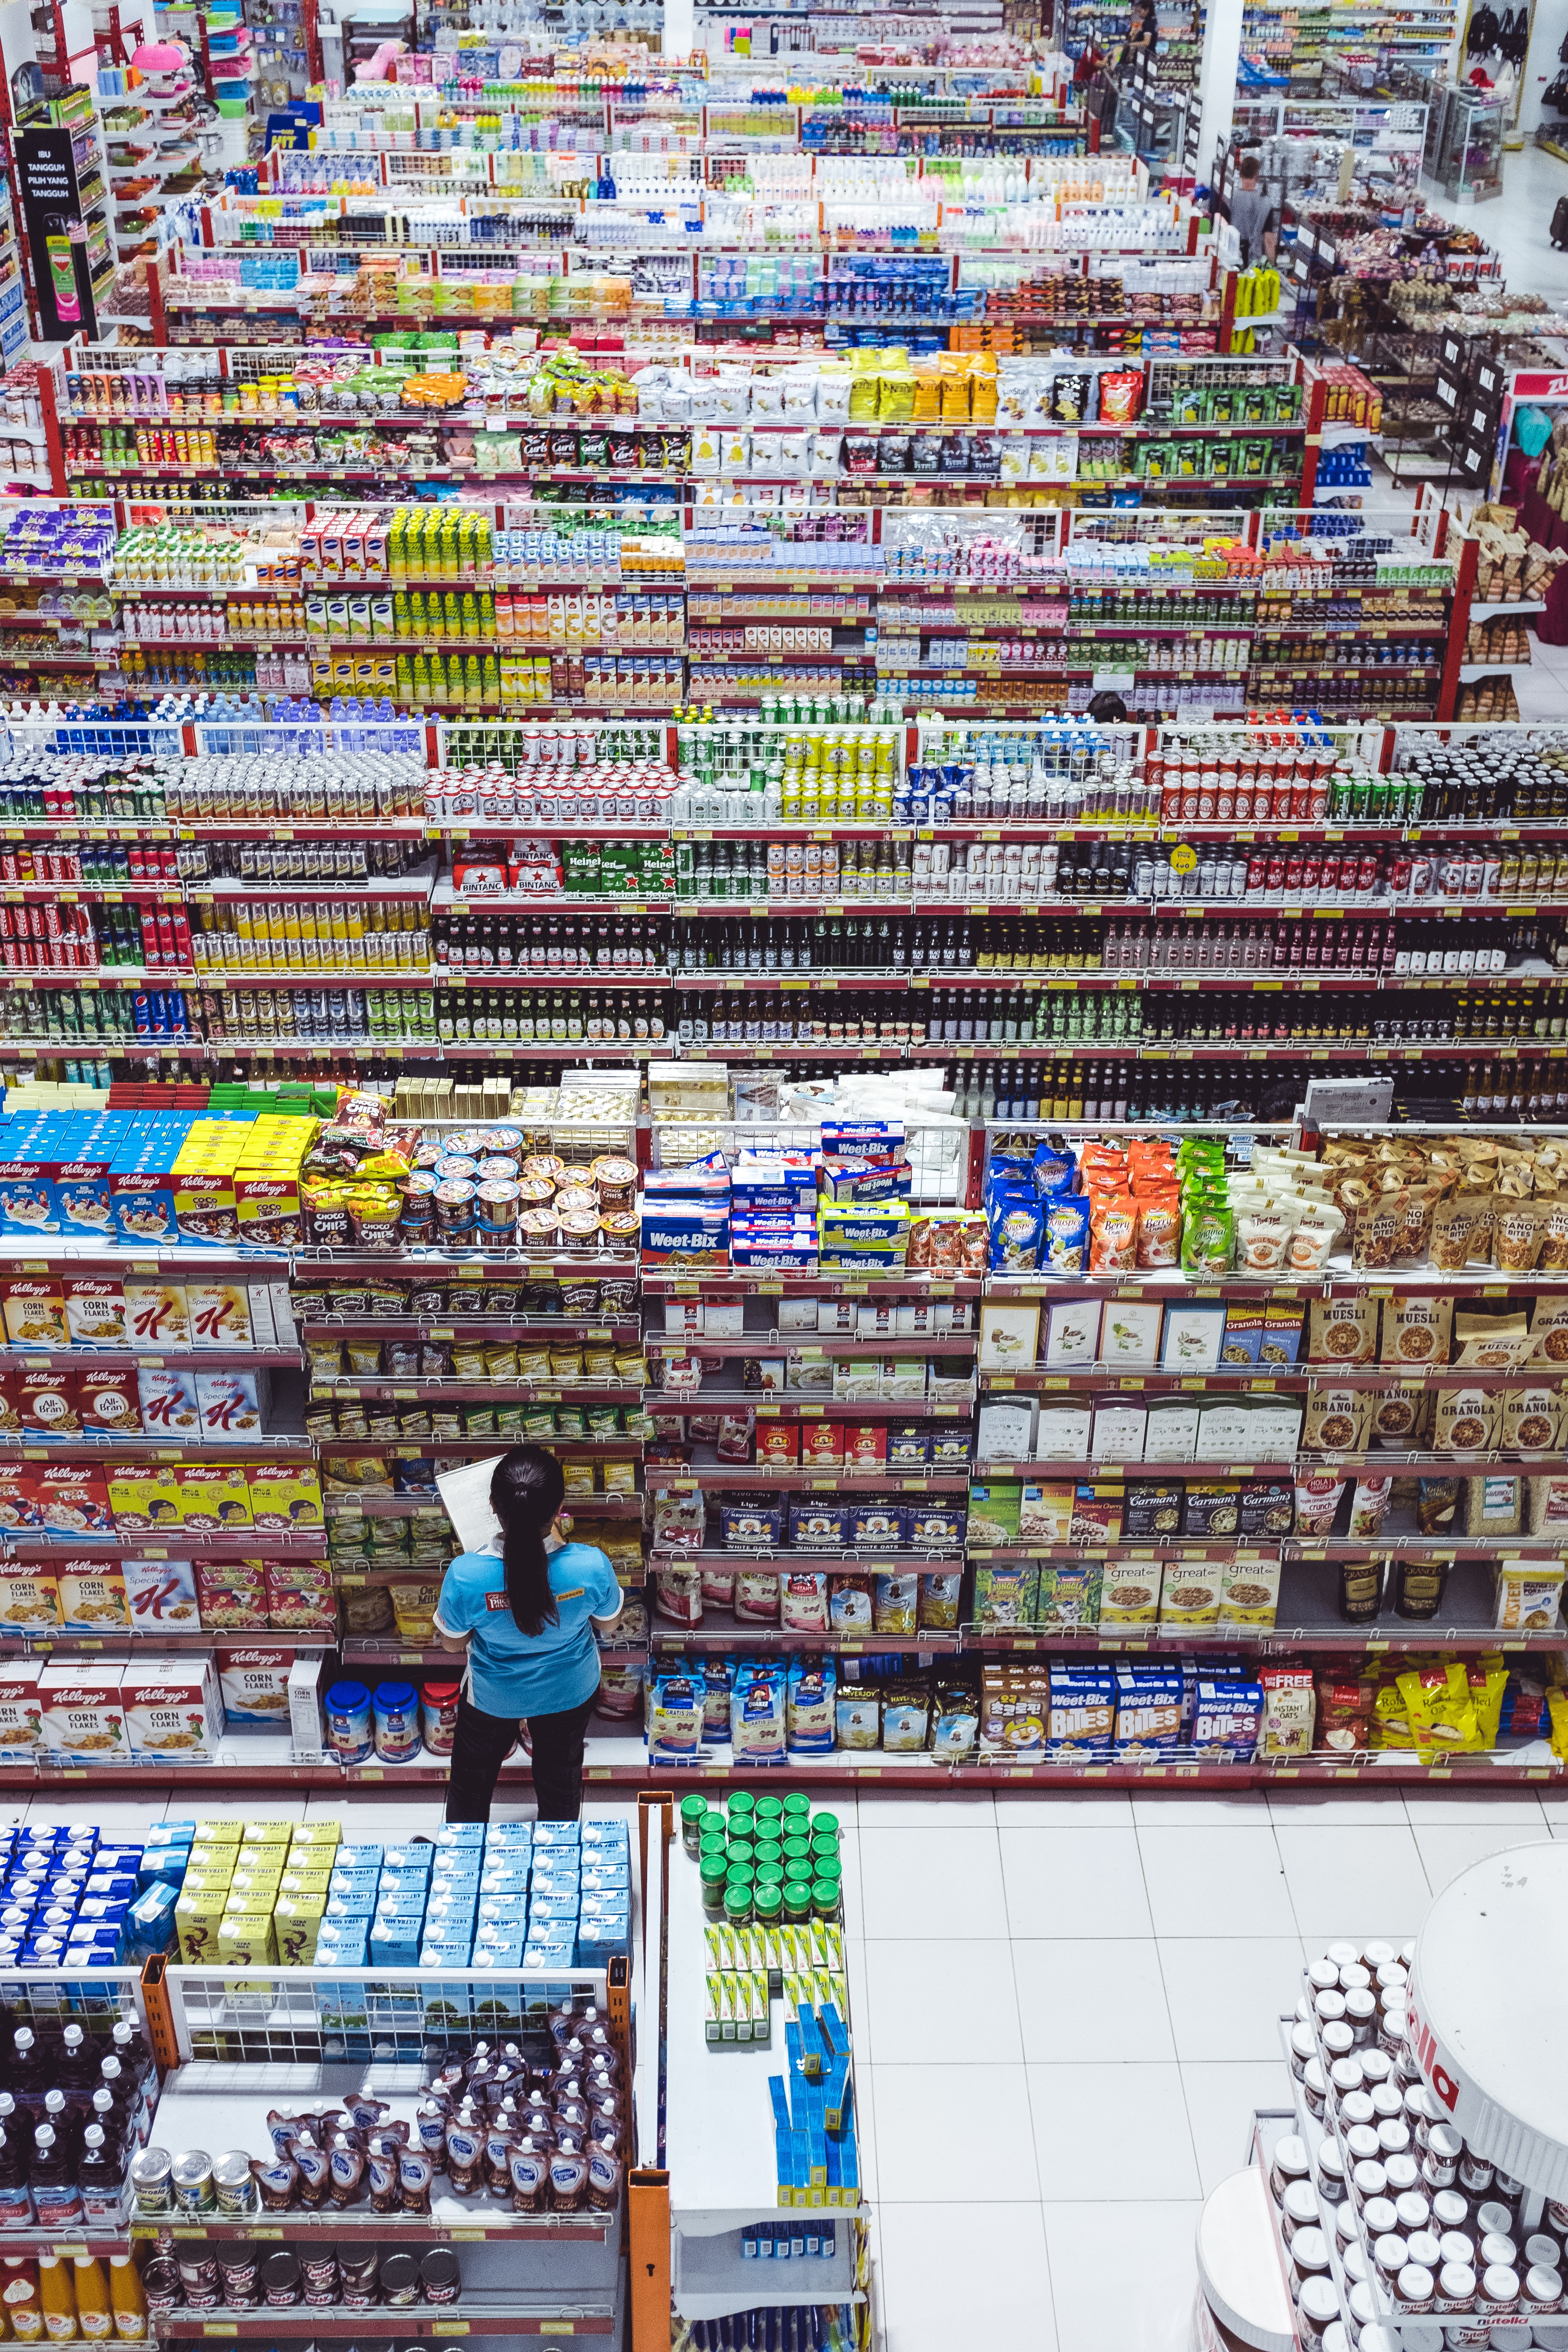
\includegraphics[width=0.4\textwidth]{gfx/09-experiment} 
\end{wrapfigure}

With thousands of products to sell, how does a merchant determine what to stock? Often that decision is the result of an experiment. The merchant may stock two or three similar items and then check to see what sells best. Part of the experiment may include manipulating the price of the items, their locations in the store, and how they are advertised. In the end, the merchant would have generated solid data to help determine what products to stock in the future.\blfootnote{Photo by Bernard Hermant on Unsplash}

Experimental research, often considered to be the ``gold standard'' in research designs by researchers who are \gls{positivist} in outlook, is one of the most rigorous of all research designs. In this design, one or more independent variables are manipulated by the researcher (``treatments''), subjects are randomly assigned to different treatment levels, and the results of the treatments on outcomes are observed and analyzed. The unique strength of experimental research is its \gls{internalvalidity} due to its ability to link cause to an effect through treatment manipulation while controlling for the spurious effect of extraneous variables.

\begin{center}
	\begin{objbox}{Objectives}
		\begin{itemize}
			\setlength{\itemsep}{0pt}
			\setlength{\parskip}{0pt}
			\setlength{\parsep}{0pt}
			
			\item Describe experimental research
			\item Define the terms control group, treatment group, treatment manipulation, random selection, validity
			\item Describe how internal validity can be improved
			\item Describe two-group designs
			\item Describe factorial designs
			\item Describe hybrid designs
			\item Describe quasi-experimental designs
			\item List the strengths and weaknesses of experimental formats
		\end{itemize}
	\end{objbox}
\end{center}

One example of experimental research can be found in Alcott's study of behavioral interventions\cite{allcott2014short}. In this study, the results of the \textit{Opower} program were evaluated. Opower was a company that sent a ``home energy report'' to more than six million homes representing $ 85 $ utilities across the United States. The reports were designed to use social pressure to get homeowners to moderate their electricity use. For Alcott's experiment, the three different sites were compared using pre- and post- intervention electricity usage statistics. He found that the initial home energy report caused high-frequency ``action and backsliding,'' but the cycles seem to attenuate over time. He also found that if the reports were discontinued the effect was still relatively persistent. Finally, he found that consumers are slow to habituate. While this study was focused on a single intervention involving energy conservation, it may be interesting to speculate if similar intervention efforts in areas like dieting, exercise, and smoking cessation would experience similar results.

Experimental research is best suited for \gls{explanatoryresearch}, where the goal of the study is to examine cause-effect relationships, rather than for descriptive or \gls{exploratoryresearch}. It also works well for research that involves a relatively limited and well-defined set of independent variables that can either be manipulated or controlled. The conduct of experimental research is generally found in one of two settings. 

\begin{itemize}
	\item Laboratory experiments, conducted in laboratory (artificial) settings, tend to be high in \gls{internalvalidity}, but this comes at the cost of low \gls{externalvalidity} because the artificial setting in which the study is conducted may not reflect the real world. As one example of a laboratory study, Berger and Iyengar\cite{berger2013communication} studied how the medium, oral vs. written, shapes the message in word-of-mouth communications. As part of their research, they conducted three laboratory studies and then collected field data to validate the laboratory studies. They found that there was a difference in how people communicated about brand name products when the channel was oral rather than written. They found, specifically, that written communication (like online chat) led to people mentioning more interesting products and brands than when they talked about them orally.

	\item Field experiments, conducted in field settings such as in an organization, can be high in \gls{externalvalidity}. But such experiments are relatively rare, because of the difficulties associated with manipulating treatments and controlling for extraneous effects in a field setting. As an example of a field experiment, Cai, Chen, and Fang\cite{cai2009observational} observed diners in restaurants to determine if knowing what other people had ordered influenced what they in turn ordered. They found that the demand for the top five dishes was increased by about $ 13 - 18\% $ when the popularity ratings were revealed to customers. 
\end{itemize}

It is common for researchers to combine experimentation settings in one project so the results of one setting can be validated in another setting. Gainsbury and Blaszczynski\cite{gainsbury2011appropriateness} specifically researched the question of whether laboratory and field experiments came to the same result. They set up a gambling laboratory and had $ 127 $ students play an electronic gambling machine that included warning about gambling presented in two different ways: pop-up and static sign. They then interviewed the gamblers to see what they remembered about the warnings. Then they went to a casino and repeated the experiment with gamblers who happened to be present. They found that the ``venue participants'' were less likely to complete surveys and when they did they provided less information than the laboratory participants. They concluded that while both settings provided valuable information about gambling behavior, care must be taken in generalizing the laboratory results to the ``real world.''

Experimental research designs can be grouped into two broad categories: true and quasi-experimental designs. Both designs require the manipulation of a treatment, but true experiments also require random assignment of participants while quasi-experiments do not. As an example of a quasi-experiment, McElroy and Morrow\cite{mcelroy2010employee} evaluated the result of an office redesign project in a large financial services company. They compared two groups of employees, those who were reassigned to a new office design and those who were not. They surveyed $ 127 $ employees who had moved and $ 144 $ who had not and then compared the perceptions of the work space and organization's culture for both groups. They found that those who moved reported less workspace and more distractions than those who did not, but the results varied by the age of the respondent. They also reported more favorable perceptions of the organization's culture and work-related attitudes with no age difference. Because the participates had not been randomly assigned to groups this was a quasi-experimental design.

\section{Basic Concepts}

All experimentation designs include the following characteristics.

\paragraph{Treatment and control groups.} In experimental research, some subjects are administered one or more experimental stimulus called a treatment (the treatment group) while other subjects are not given such a stimulus (the control group). The treatment may be considered successful if subjects in the treatment group rate more favorably on outcomes than control group subjects. Multiple levels of experimental stimulus may be administered, in which case there may be more than one treatment group. For example, in order to test the effectiveness of an advertisement, researchers may expose three different groups of people to different levels of advertising. One treatment group would view a printed article with an embedded advertisement, a second treatment group would view a television program with an embedded advertisement, and the third group, the control group, would view media with no advertising. After the exposure period, the groups could be surveyed to determine which remembered the advertising best.

\paragraph{Treatment manipulation.} Treatments are the unique feature of experimental research that sets this design apart from all other research methods. Treatment manipulation helps control for the ``cause'' in cause-effect relationships. Treatments must be checked using various pilot tests prior to the start of the experiment. Any measurements conducted before the treatment is administered to the subjects are called pretest measures and those conducted after the treatment are post-test measures. 

\paragraph{Random selection and assignment.} Random \textit{selection} is the process of randomly drawing a sample from a population or a sampling frame. This approach is typically employed in survey research and assures that each unit in the population has an equal chance of being selected into the sample. Random \textit{assignment} is the process of randomly assigning subjects to experimental or control groups. This is a standard practice in true experimental research to ensure that treatment groups are similar to each other and to the control group prior to treatment administration. Random selection is related to sampling, and is therefore, more closely related to the \gls{externalvalidity} of findings while random assignment is related to design and is related to \gls{internalvalidity}. It is common to include both random selection and random assignment in well-designed experimental research.

\paragraph{Threats to internal validity.} Although experimental designs are considered more rigorous than other research methods in terms of the internal validity of their inferences (by virtue of their ability to control causes through treatment manipulation), they are not immune to internal validity threats. As an example, imagine that researchers wanted to study the effect of a special mathematics tutoring program. They would want to plan for the following internal validity threats.

\begin{itemize}
	\item \textit{History threat} is the possibility that the observed outcomes (dependent variables) are caused by extraneous or historical events rather than by the experimental treatment. For instance, students' post-tutoring mathematics score improvement may have been caused by their preparation for a mathematics examination rather than the tutoring program.

	\item \textit{Maturation threat} refers to the possibility that observed effects are caused by natural maturation of subjects (\eg, a general improvement in their intellectual ability to understand complex concepts) rather than the experimental treatment. Perhaps the mathematics students' post-tutoring scores improved merely because they matured during the study and were better able to understand mathematics concepts.

	\item \textit{Testing threat} is a threat in pre/post designs where subjects' post-test responses are conditioned by their pretest responses. For instance, if students remember their answers from the pretest evaluation they may be able to repeat them in the post-test exam.

	\item \textit{Instrumentation threat} refers to the possibility that the difference between pretest and post-test scores is not due to the mathematics tutoring program but, rather, to changes in the administered test, such as the post-test having a higher or lower degree of difficulty than the pretest.

	\item \textit{Mortality threat} refers to the possibility that subjects may be dropping out of the study due to a systematic reason not necessarily related to the treatment. If the low-performing students drop out, the results of the post-test will be artificially inflated by the preponderance of high-performing students.

	\item \textit{Regression threat}, also called a ``regression to the mean,'' refers to the statistical tendency of a group's overall performance on a measure during a post-test to regress toward the mean of that measure rather than in the anticipated direction. For instance, if students in the mathematics study scored high on the pretest, they will have a tendency to score lower on the post-test (closer to the mean) because their initial high scores could have been a statistical aberration. It would also be true that students who under-performed on the pretest would tend to score closer to the mean on the post-test, which would falsely appear to be due to the tutoring treatment.
\end{itemize}

\section{Two-Group Experimental Designs}

The simplest true experimental designs are two group designs involving one treatment group and one control group, and are ideally suited for testing the effects of a single independent variable that can be manipulated as a treatment. The two basic two-group designs are the pretest/post-test control group design and the post-test-only control group design, while variations may include covariance designs. These designs are often depicted using a standardized design notation, where \textit{R} represents random assignment of subjects to groups, \textit{X} represents the treatment administered to the treatment group, and \textit{O} represents pretest or post-test observations of the dependent variable (with different subscripts to distinguish between pretest and post-test observations of treatment and control groups).

\paragraph{Pretest/post-test control group design.} In this design, subjects are randomly assigned to treatment and control groups, subjected to an initial (pretest) measurement of the dependent variables of interest, the treatment group is administered a treatment (representing the independent variable of interest), and the dependent variables measured again (post-test). The notation of this design is shown in Table \ref{09:tab01}, where each group's process should be read from left-to-right. Thus, the Treatment Group (top line) is first assigned using a random process, then a pretest is administered (Observation 1), then a treatment of some sort is applied, finally, a post-test is administered. The Control Group (bottom line) follows the same process, except there is no treatment applied.

\begin{table}[H]
	\centering
	\begin{tabularx}{0.85\linewidth}{p{0.10\linewidth}p{0.10\linewidth}p{0.10\linewidth}p{0.10\linewidth}p{0.40\linewidth}}
		\toprule
		\textit{R} & $ O_1 $ & \textit{X} & $ O_2 $ & \textsc{Treatment Group} \\
		\textit{R} & $ O_3 $ &            & $ O_4 $ & \textsc{Control Group} \\
		\bottomrule
	\end{tabularx}
	\caption{Pretest/Post-test Design}
	\label{09:tab01}
\end{table}

The effect, \textit{E}, of the experimental treatment in the pretest post-test design is measured as the difference in the post-test and pretest scores between the treatment and control groups, as shown in Equation \ref{09:eq01}

\begin{align}
	\label{09:eq01}
	E = (O_2 – O_1) – (O_4 – O_3)
\end{align}

Statistical analysis of this design involves a simple \gls{anova} between the treatment and control groups. The pretest post-test design mitigates several threats to internal validity, such as maturation, testing, and regression, since these threats can be expected to influence both treatment and control groups in a similar random manner. The selection threat is controlled via random assignment of members. However, additional threats to internal validity may exist. For instance, mortality can be a problem if there are differential dropout rates between the two groups, and the pretest measurement may bias the post-test measurement (especially if the pretest introduces unusual topics or content).

\paragraph{post-test-only control group design.} This design is a simpler version of the pretest/post-test design where pretest measurements are omitted. The design notation is shown in Table \ref{09:tab02}.

\begin{table}[H]
	\centering
	\begin{tabularx}{0.90\linewidth}{p{0.15\linewidth}p{0.15\linewidth}p{0.15\linewidth}p{0.40\linewidth}}
		\toprule
		\textit{R} & \textit{X} & $ O_1 $ & \textsc{Treatment Group} \\
		\textit{R} &            & $ O_2 $ & \textsc{Control Group} \\
		\bottomrule
	\end{tabularx}
	\caption{Post-test Only Design}
	\label{09:tab02}
\end{table}

The treatment effect is measured simply as the difference in the post-test scores between the two groups, as shown in Equation \ref{09:eq02}

\begin{align}
	\label{09:eq02}
	E = (O_1 – O_2)
\end{align}

The appropriate statistical analysis of this design is also a two-group \gls{anova}. The simplicity of this design makes it more attractive than the pretest/post-test design in terms of internal validity. This design controls for maturation, testing, regression, selection, and pretest/post-test interaction, though the mortality threat may continue to exist.

\paragraph{Covariance designs.} Sometimes, the measure of a dependent variable may be influenced by an extraneous variable called a \gls{covariate}. Covariates are those variables that are not of central interest to an experimental study, but should nevertheless be controlled in order to eliminate their potential effect on the dependent variable and therefore allow for a more accurate detection of the effects of the independent variables of interest. A covariance design is a special type of pretest post-test control group design where the pretest measure is essentially a measurement of the covariates of interest rather than that of the dependent variables. The design notation is shown in Table \ref{09:tab03}, where \textit{C} represents the covariates:

\begin{table}[H]
	\centering
	\begin{tabularx}{0.85\linewidth}{p{0.10\linewidth}p{0.10\linewidth}p{0.10\linewidth}p{0.10\linewidth}p{0.40\linewidth}}
		\toprule
		\textit{R} & \textit{C} & \textit{X} & $ O_1 $ & \textsc{Treatment Group} \\
		\textit{R} & \textit{C} &            & $ O_2 $ & \textsc{Control Group} \\
		\bottomrule
	\end{tabularx}
	\caption{Covariate Design}
	\label{09:tab03}
\end{table}

Because the pretest measure is not a measurement of the dependent variable, but rather a covariate, the treatment effect is measured as the difference in the post-test scores between the treatment and control groups as in Equation \ref{09:eq03}.

\begin{align}
	\label{09:eq03}
	E = (O_1 – O_2)
\end{align}

Due to the presence of covariates, the right statistical analysis of this design is a two-group \gls{ancova}. This design has all the advantages of post-test only design, but with internal validity due to the controlling of covariates. Covariance designs can also be extended to pretest/post-test control group design.

\section{Factorial Designs}

Two-group designs are inadequate if the research project requires manipulation of two or more independent variables (treatments). In such cases, four or higher-group designs are required. Such designs, quite popular in experimental research, are commonly called \glspl{factorialdesign}. Each independent variable in this design is called a factor, and each sub-division of a factor is called a level. Factorial designs enable researchers to examine not only the individual effect of each treatment on the dependent variables (called main effects), but also their joint effect (called interaction effects).

The most basic factorial design is a $ 2 x 2 $ factorial design, which consists of two treatments, each with two levels (such as high/low or present/absent). For instance, suppose a research project compares the learning outcomes of two different types of instructional techniques (online and in-class) along with the time of instruction ($ 1.5 $ or $ 3 $ hours per week). In this case, there are two factors: instructional type and instructional time; each with two levels (in-class and online for instructional type, and $ 1.5 $ and $ 3 $ hours/week for instructional time), as shown in Figure \ref{09:fig01}. If a third level of instructional time (maybe $ 6 $ hours/week) is desired then the second factor will consist of three levels and a $ 2 x 3 $ factorial design is required. On the other hand, if a third factor, such as group work (present versus absent), is desired, then a $ 2 x 2 x 2 $ factorial design is needed. In this notation, each number represents a factor, and the value of each factor represents the number of levels in that factor.

\begin{center}
	\begin{figure}[H]
		\tikzstyle{tlbox}=[rectangle,draw=blue!50,fill=blue!20,ultra thick,
		inner sep=10pt,minimum width=4.5cm,minimum height=2.0cm,
		rounded corners=.25cm]
		\tikzstyle{trbox}=[rectangle,draw=red!50,fill=red!20,ultra thick,
		inner sep=10pt,minimum width=4.5cm,minimum height=2.0cm,
		rounded corners=.25cm]
		\tikzstyle{blbox}=[rectangle,draw=green!50,fill=green!20,ultra thick,
		inner sep=10pt,minimum width=4.5cm,minimum height=2.0cm,
		rounded corners=.25cm]
		\tikzstyle{brbox}=[rectangle,draw=yellow!50,fill=yellow!20,ultra thick,
		inner sep=10pt,minimum width=4.5cm,minimum height=2.0cm,
		rounded corners=.25cm]			
		\tikzstyle{every label}=[red]
		\begin{tikzpicture}
		\node[tlbox] (gp1)                      {Group 1};
		\node[trbox] (gp2) [right=0.5cm of gp1] {Group 2};
		\node[blbox] (gp3) [below=0.5cm of gp1]	{Group 3};
		\node[brbox] (gp4) [right=0.5cm of gp3] {Group 4};
		
		\node[] (ttext1) [above=1.0cm of gp1,xshift=2.5cm] {Instructional Time};
		\node[] (ttext2) [above=0.5cm of gp1,yshift=-0.25cm] {1.5 hours/wk};		
		\node[] (ttext3) [above=0.5cm of gp2,yshift=-0.25cm] {3.0 hours/wk};		
		\node[] (ltext1) [left=1.0cm of gp1,yshift=0.50cm,rotate=90] {Instructional Type};
		\node[] (ltext2) [left=0.5cm of gp1,yshift=0.75cm,rotate=90] {Online};
		\node[] (ltext3) [left=0.5cm of gp3,yshift=0.75cm,rotate=90] {In-class};
		
		\node[] (factor) [red,left=3.0cm of ttext1] {Factors};
		\node[] (level)  [blue, left=2.5cm of ttext1,yshift=-0.68cm] {Levels};

		% Arrows		
		\draw [->,red,line width=1pt] (factor) to (ttext1);
		\draw (-3.25cm, 2.10cm) [->,red,line width=1pt] to (ltext1.east);
		\draw [->,blue,line width=1pt] (level) to (ttext2);
		\draw (-2.775cm, 1.30cm) [->,blue,line width=1pt] to (ltext2.east);
		
		
		\end{tikzpicture}
		\caption{2X2 Factorial Design}
		\label{09:fig01}
	\end{figure}
\end{center}

Factorial designs can also be depicted using a design notation, such as that shown in Table \ref{09:tab04}. 

\begin{table}[H]
	\centering
	\begin{tabularx}{0.75\linewidth}{p{0.15\linewidth}p{0.15\linewidth}p{0.15\linewidth}p{0.25\linewidth}}
		\toprule
		\textit{R} & $ X_{11} $ & $ O_1 $ & \textsc{Group 1} \\
		\textit{R} & $ X_{12} $ & $ O_2 $ & \textsc{Group 2} \\
		\textit{R} & $ X_{21} $ & $ O_3 $ & \textsc{Group 3} \\
		\textit{R} & $ X_{22} $ & $ O_4 $ & \textsc{Group 4} \\
		\bottomrule
	\end{tabularx}
	\caption{2X2 Factorial Design}
	\label{09:tab04}
\end{table}

\textit{R} represents random assignment of subjects to treatment groups, \textit{X} represents the treatment groups themselves (the subscripts of \textit{X} represents the level of each factor), and \textit{O} represent observations of the dependent variable. Notice that the $ 2 x 2 $ factorial design will have four treatment groups, corresponding to the four combinations of the two levels of each factor. Correspondingly, a $ 2 x 3 $ design will have six treatment groups, and a $ 2 x 2 x 2 $ design will have eight treatment groups. As a rule of thumb, each cell in a factorial design should have a minimum sample size of $ 20 $ (this estimate is derived from Cohen's power calculations based on medium effect sizes). So a $ 2 x 2 x 2 $ factorial design requires a minimum total sample size of $ 160 $ subjects, with at least $ 20 $ subjects in each cell. It is obvious that the cost of data collection can increase substantially with more levels or factors in a factorial design. Sometimes, due to resource constraints, some cells in such factorial designs may not receive any treatment at all, which are called \textit{incomplete factorial designs}, but incomplete designs decrease the ability to draw inferences about the those factors.

In a factorial design, a \textit{main effect} is said to exist if the dependent variable shows a significant difference between multiple levels of one factor and at all levels of other factors. No change in the dependent variable across factor levels is the null case (baseline), from which main effects are evaluated. In the above example, perhaps a main effect of instructional type, instructional time, or both can be seen on learning outcomes. An \textit{interaction effect} exists when the effect of differences in one factor depends upon the level of a second factor. In the above example, if the effect of instructional type on learning outcomes is greater for $ 3 $ hours/week of instructional time than for $ 1.5 $ hours/week, then there is an interaction effect between instructional type and instructional time on learning outcomes. Note that the presence of interaction effects dominate and make main effects irrelevant, and it is not meaningful to interpret main effects if interaction effects are significant.

\section{Hybrid Experimental Designs}

Hybrid designs are those that are formed by combining features of more established designs. Three such hybrid designs are randomized blocks design, Solomon four-group design, and switched replications design.

\paragraph{Randomized block design.} This is a variation of the post-test-only or pretest/post-test control group design where the subject population can be grouped into relatively homogeneous subgroups (called blocks) within which the experiment is replicated. For instance, to replicate the same post-test-only design among university students and full-time working professionals (two homogeneous blocks), subjects in both blocks are randomly split between a treatment group (receiving the same treatment) or control group (see Table \ref{09:tab05}). The purpose of this design is to reduce the ``noise'' or variance in data that may be attributable to differences between the blocks so that the actual effect of interest can be detected more accurately.

\begin{table}[H]
	\centering
	\begin{tabularx}{0.90\linewidth}{p{0.40\linewidth}p{0.15\linewidth}p{0.15\linewidth}p{0.15\linewidth}}
		\toprule
		\textsc{University Students} & \textit{R} & $ X $ & $ O_1 $ \\
		\textsc{University Students} & \textit{R} &       & $ O_2 $ \\
		\textsc{Professionals} & \textit{R} & $ X $ & $ O_3 $ \\
		\textsc{Professionals} & \textit{R} &       & $ O_4 $ \\
		\bottomrule
	\end{tabularx}
	\caption{Randomized Block Design}
	\label{09:tab05}
\end{table}

\paragraph{Solomon four-group design.} In this design, the sample is divided into two treatment groups and two control groups. One treatment group and one control group receive the pretest, and the other two groups do not. This design represents a combination of post-test-only and pretest/post-test control group design, and is intended to test for the potential biasing effect of pretest measurement on post-test measures that tends to occur in pretest/post-test designs but not in post-test only designs. The design notation is shown in Table \ref{09:tab06}.

\begin{table}[H]
	\centering
	\begin{tabularx}{0.65\linewidth}{p{0.15\linewidth}p{0.15\linewidth}p{0.15\linewidth}p{0.15\linewidth}}
		\toprule
		\textit{R} & $ O_1 $ & $ X $ & $ O_2 $ \\
		\textit{R} & $ O_3 $ &       & $ O_4 $ \\
		\textit{R} &         & $ X $ & $ O_5 $ \\
		\textit{R} &         &       & $ O_6 $ \\
		\bottomrule
	\end{tabularx}
	\caption{Solomon Four-group Design}
	\label{09:tab06}
\end{table}

\paragraph{Switched replication design.} This is a two-group design implemented in two phases with three waves of measurement. The treatment group in the first phase serves as the control group in the second phase, and the control group in the first phase becomes the treatment group in the second phase, as illustrated in Table \ref{09:tab07}. In other words, the original design is repeated or replicated temporally with treatment/control roles switched between the two groups. By the end of the study, all participants will have received the treatment either during the first or the second phase. This design is most feasible in organizational contexts where organizational programs (e.g., employee training) are implemented in a phased manner or are repeated at regular intervals.

\begin{table}[H]
	\centering
	\begin{tabularx}{0.75\linewidth}{p{0.10\linewidth}p{0.10\linewidth}p{0.10\linewidth}p{0.10\linewidth}p{0.10\linewidth}p{0.10\linewidth}}
		\toprule
		\textit{R} & $ O_1 $ & $ X $ & $ O_2 $ &       & $ O_3 $ \\
		\textit{R} & $ O_4 $ &       & $ O_5 $ & $ X $ & $ O_6 $ \\
		\bottomrule
	\end{tabularx}
	\caption{Switched Replication Design}
	\label{09:tab07}
\end{table}

\section{Quasi-Experimental Designs}

Quasi-experimental designs are almost identical to true experimental designs, but lacking one key ingredient: random assignment. For instance, one entire class section or one organization is used as the treatment group, while another section of the same class or a different organization in the same industry is used as the control group. This lack of random assignment potentially results in groups that are non-equivalent, such as one group possessing greater mastery of a certain content than the other group, say by virtue of having a better teacher in a previous semester, which introduces the possibility of selection bias. Quasi-experimental designs are therefore inferior to true experimental designs in interval validity due to the presence of a variety of selection related threats such as selection-maturation threat (the treatment and control groups maturing at different rates), selection-history threat (the treatment and control groups being impacted differently by extraneous or historical events), selection-regression threat (the treatment and control groups regressing toward the mean between pretest and post-test at different rates), selection-instrumentation threat (the treatment and control groups responding differently to the measurement), selection-testing (the treatment and control groups responding differently to the pretest), and selection mortality (the treatment and control groups demonstrating differential dropout rates). Given these selection threats, it is generally preferable to avoid quasi-experimental designs.

Many true experimental designs can be converted to quasi-experimental designs by omitting random assignment. For instance, the quasi-equivalent version of pretest/post-test control group design is called \gls{negd}, as shown in Table \ref{09:tab08}, with random assignment \textit{R} replaced by non-equivalent (non-random) assignment \textit{N}. Likewise, the quasi-experimental version of switched replication design is called \textit{Nonequivalent Switched Replication Design} (see Table \ref{09:tab09}).

\begin{table}[H]
	\centering
	\begin{tabularx}{0.85\linewidth}{p{0.10\linewidth}p{0.10\linewidth}p{0.10\linewidth}p{0.10\linewidth}p{0.40\linewidth}}
		\toprule
		\textit{N} & $ O_1 $ & \textit{X} & $ O_2 $ & \textsc{Treatment Group} \\
		\textit{N} & $ O_3 $ &            & $ O_4 $ & \textsc{Control Group} \\
		\bottomrule
	\end{tabularx}
	\caption{Nonequivalent Groups Design}
	\label{09:tab08}
\end{table}


\begin{table}[H]
	\centering
	\begin{tabularx}{0.75\linewidth}{p{0.10\linewidth}p{0.10\linewidth}p{0.10\linewidth}p{0.10\linewidth}p{0.10\linewidth}p{0.10\linewidth}}
		\toprule
		\textit{N} & $ O_1 $ & $ X $ & $ O_2 $ &       & $ O_3 $ \\
		\textit{N} & $ O_4 $ &       & $ O_5 $ & $ X $ & $ O_6 $ \\
		\bottomrule
	\end{tabularx}
	\caption{Nonequivalent Switched Replication Design}
	\label{09:tab09}
\end{table}

In addition, there are quite a few unique non-equivalent designs without corresponding true experimental design cousins, including those listed below.

\paragraph{\gls{rd} design.} This is a non-equivalent pretest/post-test design where subjects are assigned to treatment or control group based on a cutoff score on a pre-program measure. For instance, patients who are severely ill may be assigned to a treatment group to test the efficacy of a new drug or treatment protocol and those who are mildly ill are assigned to the control group. In another example, students who are lagging behind on standardized test scores may be selected for a remedial curriculum program intended to improve their performance, while those who score high on such tests are not selected from the remedial program. The design notation can be represented as in Table \ref{09:tab10}, where \textit{C} represents the cutoff score:

\begin{table}[H]
	\centering
	\begin{tabularx}{0.85\linewidth}{p{0.10\linewidth}p{0.10\linewidth}p{0.10\linewidth}p{0.10\linewidth}p{0.40\linewidth}}
		\toprule
		\textit{C} & $ O_1 $ & \textit{X} & $ O_2 $ & \textsc{Treatment Group} \\
		\textit{C} & $ O_3 $ &            & $ O_4 $ & \textsc{Control Group} \\
		\bottomrule
	\end{tabularx}
	\caption{Regression-discontinuity Design}
	\label{09:tab10}
\end{table}

Because of the use of a cutoff score, it is possible that the observed results may be a function of the cutoff score rather than the treatment, which introduces a new threat to internal validity. However, using the cutoff score also ensures that limited or costly resources are distributed to people who need them the most rather than randomly across a population, while simultaneously allowing a quasi-experimental treatment. The control group scores in the \gls{rd} design do not serve as a benchmark for comparing treatment group scores, given the systematic non-equivalence between the two groups. Rather, if there is no discontinuity between pretest and post-test scores in the control group, but such a discontinuity persists in the treatment group, then this discontinuity is viewed as evidence of the treatment effect.

\paragraph{Proxy pretest design.} This design, shown in Table \ref{09:tab11}, looks very similar to the standard \gls{negd} (pretest-post-test) design, with one critical difference: the pretest score is collected after the treatment is administered. A typical application of this design is when a researcher is brought in to test the efficacy of a program (\eg, an educational program) after the program has already started and pretest data is not available. Under such circumstances, the best option for the researcher is often to use a different prerecorded measure, such as students' grade point averages before the start of the program, as a proxy for pretest data. A variation of the proxy pretest design is to use subjects' post-test recollection of pretest data, which may be subject to recall bias, but nevertheless may provide a measure of perceived gain or change in the dependent variable.

\begin{table}[H]
	\centering
	\begin{tabularx}{0.85\linewidth}{p{0.10\linewidth}p{0.10\linewidth}p{0.10\linewidth}p{0.10\linewidth}p{0.40\linewidth}}
		\toprule
		\textit{N} & $ O_1 $ & \textit{X} & $ O_2 $ & \textsc{Treatment Group} \\
		\textit{N} & $ O_3 $ &            & $ O_4 $ & \textsc{Control Group} \\
		\bottomrule
	\end{tabularx}
	\caption{Proxy Pretest Design}
	\label{09:tab11}
\end{table}

\paragraph{Separate pretest/post-test samples design.} This design is useful if it is not possible to collect pretest and post-test data from the same subjects for some reason. As shown in Table \ref{09:tab12}, there are four groups in this design, but two groups come from a single non-equivalent group, while the other two groups come from a different non-equivalent group. For instance, to test customer satisfaction with a new online service that is implemented in one city but not in another, customers in the first city serve as the treatment group and those in the second city constitute the control group. If it is not possible to obtain pretest and post-test measures from the same customers, you can measure customer satisfaction at one point in time, implement the new service program, and measure customer satisfaction (with a different set of customers) after the program is implemented. Customer satisfaction is also measured in the control group at the same times as in the treatment group, but without the new program implementation. The design is not particularly strong, because changes in any specific customer's satisfaction score before and after the implementation cannot be examined, only the average customer satisfaction scores. Despite the lower internal validity, this design may still be a useful way of collecting quasi-experimental data when pretest and post-test data are not available from the same subjects.

\begin{table}[H]
	\centering
	\begin{tabularx}{0.65\linewidth}{p{0.15\linewidth}p{0.15\linewidth}p{0.15\linewidth}p{0.15\linewidth}}
		\toprule
		$ N_1 $ & $ O_1 $  &       &         \\
		$ N_1 $ &          & $ X $ & $ O_2 $ \\
		$ N_2 $ & $ O_3 $  &       &         \\
		$ N_2 $ &          &       & $ O_4 $ \\
		\bottomrule
	\end{tabularx}
	\caption{Separate Pretest/Posttest Samples Design}
	\label{09:tab12}
\end{table}

\paragraph{\gls{nedv} design.} This is a single-group pre/post quasi-experimental design with two outcome measures, where one measure is theoretically expected to be influenced by the treatment and the other measure is not. For instance, if a new calculus curriculum is being designed for high school students, the curriculum is anticipated to influence students' post-test calculus scores but not algebra scores. However, the post-test algebra scores may still vary due to extraneous factors such as history or maturation. Hence, the pre/post algebra scores can be used as a control measure, while the pre/post calculus scores can be treated as the treatment measure. The design notation, shown in Table \ref{09:tab13}, indicates the single group, \textit{N}, followed by pretest $ O_1 $ and post-test $ O_2 $ for both calculus and algebra for the same group of students. This design is weak in internal validity, but its advantage lies in not having to use a separate control group.

An interesting variation of the \gls{nedv} design is a pattern matching \gls{nedv} design, which employs multiple outcome variables and a theory that explains how much each variable will be affected by the treatment. The researcher can then examine if the theoretical prediction is matched in actual observations. This pattern-matching technique, based on the degree of correspondence between theoretical and observed patterns is a powerful way of alleviating internal validity concerns in the original \gls{nedv} design.

\begin{table}[H]
	\centering
	\begin{tabularx}{0.65\linewidth}{p{0.15\linewidth}p{0.15\linewidth}p{0.15\linewidth}p{0.15\linewidth}}
		\toprule
		\multirow{2}{*}{$ N $} & $ O_1 $ & $ X $ & $ O_2 $ \\
		                       & $ O_3 $ &       & $ O_4 $ \\
		\bottomrule
	\end{tabularx}
	\caption{Nonequivalent Dependent Variable Design}
	\label{09:tab13}
\end{table}

\section{Strengths and Weaknesses of Experimental Research}

A strength of the experimental method, particularly in cases where experiments are conducted in lab settings, is that the researcher has substantial control over the conditions to which participants are subjected. Experiments are also generally easier to replicate than are other methods of data collection, especially in cases where an experiment has been conducted in a lab setting.

On the other hand, experimental research is one of the most difficult of research designs, and should not be taken lightly. This type of research is often beset with a multitude of methodological problems. 

\begin{itemize}
	\item Though experimental research requires theories for framing hypotheses for testing, much of current experimental research is atheoretical. Without theories, the hypotheses being tested tend to be ad hoc, possibly illogical, and meaningless. 

	\item Many of the measurement instruments used in experimental research are not tested for reliability and validity and are incomparable across studies. Consequently, results generated using such instruments are also incomparable. 

	\item Many experimental research use inappropriate research designs, such as irrelevant dependent variables, no interaction effects, no experimental controls, and nonequivalent stimulus across treatment groups. Findings from such studies tend to lack internal validity and are highly suspect. 

	\item The treatments (tasks) used in experimental research may be diverse, incomparable, and inconsistent across studies and sometimes inappropriate for the subject population. For instance, undergraduate student subjects are often asked to pretend that they are marketing managers and asked to perform a complex budget allocation task in which they have no experience or expertise. The use of such inappropriate tasks introduces new threats to internal validity (\ie, subject's performance may be an artifact of the content or difficulty of the task setting), generates findings that are non-interpretable and meaningless, and makes integration of findings across studies impossible.
\end{itemize}

The design of proper experimental treatments is a very important task in experimental design, because the treatment is the raison d'\^{e}tre of the experimental method, and must never be rushed or neglected. To design an adequate and appropriate task, researchers should use pre-validated tasks if available, conduct treatment manipulation checks to check for the adequacy of such tasks (by debriefing subjects after performing the assigned task), conduct pilot tests (repeatedly, if necessary), and if there is doubt, using tasks that are simpler and familiar for the respondent sample than tasks that are complex or unfamiliar.

Time, other resources such as funding, and even the topic may limit a researcher's ability to conduct an experiment. For researchers in the medical and health sciences, conducting an experiment could require denying needed treatment to patients, which is a clear ethical consideration. Even those whose research may not involve the administration of medications or treatments may be limited in their ability to conduct a classic experiment. In business or economics experiments, for example, it may not be ethical to provide a financial or other reward to members of the experimental group but not the control group. 

\section{Summary}\label{ch09:summary}

\begin{center}
	\begin{tkawybox}{Summary}
		\begin{itemize}
			\setlength{\itemsep}{0pt}
			\setlength{\parskip}{0pt}
			\setlength{\parsep}{0pt}
			
			\item Describe experimental research
			\item Define the terms control group, treatment group, treatment manipulation, random selection, validity
			\item Describe how internal validity can be improved
			\item Describe two-group designs
			\item Describe factorial designs
			\item Describe hybrid designs
			\item Describe quasi-experimental designs
			\item List the strengths and weaknesses of experimental formats
			
		\end{itemize}
	\end{tkawybox}
\end{center}


\ctparttext{Qualitative methods are based in the evaluation of non-numeric data, like photographs and text documents. These methods include activities like field work, unobtrusive, and interpretive research methods.}
\part{Qualitative Methods}
\cleardoublepage
\include{Chapters/10Interviews}
%*****************************************
\chapter{Field Research}\label{ch11:field_research}
%*****************************************
\section{Introduction}

\begin{wrapfigure}{r}{0.4\textwidth}
	\centering
	\includegraphics[width=0.4\textwidth]{gfx/11-mop} 
\end{wrapfigure}

If researchers wanted to know who conducts more of the housework in households, how could they find the answer? One way might be to interview people and simply ask them. That is exactly what Arlie Hochschild did in her study of the second shift, her term for the work that goes on in the home after the day's work for pay is completed\cite{hochschild2012second}. Hochschild interviewed $ 50 $ heterosexual, married couples with children to learn about how they did, or did not, share the work of the second shift. Many of these couples reported to her that they shared the load of the second shift equally, sometimes dividing the house into areas that were ``her responsibility'' and those that were ``his.'' But Hochschild was not satisfied with just people's personal accounts of second-shift work. She chose to observe $ 12 $ of these couples in their homes as well, to see for herself just how the second shift was shared.\blfootnote{Photo by rawpixel on Unsplash}

What Hochschild discovered was that even those couples who claimed to share the second shift did not have as equitable a division of duties as they had professed. For example, one couple who told Hochschild during their interview that they shared the household work equally had explained that the wife was responsible for the upstairs portion of the house and the husband took responsibility for the downstairs portion. Upon conducting observations in this couple's home, however, Hochschild discovered that the upstairs portion of the house contained all the bedrooms and bathrooms, the kitchen, the dining room, and the living room, while the downstairs included a storage space and the garage. This division of labor meant that the woman actually carried the weight of responsibility for the second shift. Without a field research component to her study, Hochschild might never have uncovered these and other truths about couples' behaviors and sharing (or not sharing) of household duties.

\begin{center}
	\begin{objbox}{Objectives}
		\begin{itemize}
			\setlength{\itemsep}{0pt}
			\setlength{\parskip}{0pt}
			\setlength{\parsep}{0pt}
			
			\item Define ``Field Research.''
			\item Describe the strengths and weaknesses of field research.
			\item Describe how to get started with field research: choosing a site and role.
			\item Describe how to write field notes and then analyze those notes.
		\end{itemize}
	\end{objbox}
\end{center}


\section{What Is Field Research?}

Field research is a qualitative method of data collection aimed at understanding, observing, and interacting with people in their natural settings. Thus when researchers talk about being in ``the field,'' they're talking about being out in the real world and involved in the everyday lives of the people they are studying. Two terms are commonly used to describe this type of project, field research and participant observation. Field research is an umbrella term that includes the myriad activities that field researchers engage in when they collect data: they participate, they observe, they usually interview some of the people they observe, and they typically analyze documents or artifacts created by the people they observe.

Because interviews (Chapter \ref{ch10:interviews}) and document analysis (Chapter \ref{ch12:unobtrusive}) are covered elsewhere, this chapter focuses only on the participation and observation aspects of field research. These aspects of field research are usually considered together and are known as \textit{participant observation}. Like field research, participant observation also has multiple meanings. Researchers conducting participant observation vary in the extent to which they participate or observe\cite{baker2006observation}. While many ``participation scales'' have been developed, Baker proposes a continuum where ``Nonparticipation'' lies at one end and ``complete membership'' lies at the other, as illustrated in Figure \ref{11:fig01}.\label{11:continuum}

\begin{center}
	\begin{figure}[H]
		\begin{tikzpicture}
		% Yellow Rectangle
		\shade[left color=white!25!yellow, right color=white!75!yellow] (0,0) rectangle +(11cm, 4.5cm);

		% Text Nodes
		\tikzset{anchor=west}
		\node[rotate=90] at (1cm,0) {Nonparticipation};
		\node[rotate=90] at (2.5cm,0) {Complete Observer};
		\node[rotate=90] at (4.0cm,0) {Observer-as-Participant};
		\node[rotate=90] at (5.5cm,0) {Moderate Membership};
		\node[rotate=90] at (7.0cm,0) {Participant-as-Observer};
		\node[rotate=90] at (8.5cm,0) {Complete Participation};
		\node[rotate=90] at (10cm,0) {Complete Membership};

		% Horizontal Arrow
		\draw [<->, blue, line width=3pt, opacity=0.2] (0cm,2.25cm) to (11cm,2.25cm);
		
		\end{tikzpicture}
		\caption{Participant Observation Levels}
		\label{11:fig01}
	\end{figure}
\end{center}


\begin{description}

	\item[Nonparticipation] Researchers using this method have no involvement with the group being studied. Researchers are not physically present but can observe using an entirely different environment. As an example of this level of involvement, imagine a researcher watching some sort of group interaction from another room on a closed-circuit television system.

	\item[Complete Observer] Researchers using this method are physically present with the insiders being observed but have no interaction (or, at most, minimal superficial interaction) with the insiders. Researchers are only present to listen and observe.

	\item[Observer-as-Participant] Researchers using this method are engaged in more observation than participation but still have some interaction, like brief interviews, with the insiders. Researchers do not become friends with the insiders and would not ``get a beer after work'' but would feel comfortable asking them why they were doing some task in a particular manner. 

	\item[Moderate Membership] Researchers using this method attempt to maintain a balance between being an insider and pure observation. They would participate in certain activities but not those that are at the core of insider membership. As an example, researchers observing drug dealers may ``hang out'' and listen to music with them, but would not engage in any sort of illegal activity.

	\item[Participant-as-Observer] Researchers using this method become more involved with insiders' central activities but still do not fully commit to the members' values and goals. Researchers may develop friendships with the insiders and even participate in social activities, like going to dinner together, with them.

	\item[Complete Participation] Researchers using this method are said to ``go native'' with the insiders. They become part of the insiders' group and share all of the goals and norms of the group being studied. This level of involvement can be problematic since researchers may become so ingrained in the group being observed that they can no longer offer unbiased observations. For this reason, most research experts warn that ``going native'' should be avoided.

	\item[Complete Membership] Researchers using this method have completely ``gone native'' and are part of the group being observed. The main difference between this level and the previous level is that researchers who attain complete membership do so intentionally and have no hesitation in being part of the group being observed.

\end{description}

As it might have been imagined based on the examples of the observational roles assumed, field research is well equipped to answer ``how'' kinds of questions. Whereas survey researchers often aim to answer ``why'' questions, field researchers ask how the processes they study occur, how the people they spend time with in the field interact, and how events unfold. 

Field research is a method that was originally crafted by anthropologists for the purpose of cultural understanding and interpretation\cite{wolcott1999ethnography}. Dissatisfied with studying groups of people based solely on secondhand accounts and inspection of artifacts, several anthropologists decided to try living in or near the communities they studied to learn from and about them. Two anthropologists in particular, Franz Boas\cite{boas1964central} and Bronislaw Malinowski\cite{malinowski2014argonauts} are credited with developing this method around the turn of the $ 20 $th century. Boas lived with native populations in Canada and in the American Northwest. Malinowski lived in Papua New Guinea with people who were native to the area. Sociologists picked up on the idea and on the benefits of field research. Soon, a number of sociologists had embraced this new method and adapted field research for their own studies of groups. Many of the early field researchers in sociology were former social workers who got interested in sociological research because of experiences in their roles as social reformers. 

\section{Strengths and Weaknesses of Field Research}

Like any research method, field research has both benefits and drawbacks.

\subsection{Strengths of Field Research}

Field research allows researchers to gain firsthand experience and knowledge about the people, events, and processes that they study. No other method offers quite the same kind of closeup lens on everyday life. This close-up on everyday life means that field researchers can obtain very detailed data about people and processes, perhaps more detailed than they can obtain using any other method.

Field research is an excellent method for understanding the role of social context in shaping people's lives and experiences. It enables a greater understanding of the intricacies and complexities of daily life. Field research may also uncover elements of people's experiences or of group interactions of which we were not previously aware. This in particular is a unique strength of field research. With other methods, such as interviews and surveys, respondents cannot answer questions to which they do not know the answer or to provide us with information of which they are not aware. Also, because field research typically occurs over an extended period of time, social facts that may not even be immediately revealed to a researcher but that become discovered over time can be uncovered during the course of a field research project.

In sum, the major benefits of field research are the following:

\begin{enumerate}
	\item It yields very detailed data.
	\item It emphasizes the role and relevance of social context.
	\item It can uncover social facts that may not be immediately obvious or of which research participants may be unaware.
\end{enumerate}

\subsection{Weaknesses of Field Research}

Despite the fact that field researchers can collect very detailed data, that comes at a cost. Because a field researcher's focus is so detailed, it is by necessity also somewhat narrow. Field researchers simply are not able to gather data from as many individuals as opposed to a survey, for example. Indeed, field researchers generally sacrifice breadth in exchange for depth. Related to this point is the fact that field research is extremely time intensive.

Field research can also be emotionally taxing. Interview research requires, to a certain extent, the development of a relationship between a researcher and her participants, but field research requires a much greater investment in the researcher's life. It may be said that interviews are like casual dating while field research is like a marriage.

The relationships developed as a field researcher are sustained over a much longer period than the hour or two it might take to conduct an interview. Not only do the relationships last longer, but they are also more intimate. A number of field researchers have documented the complexities of relationships with research participants (See Taylor\cite{taylor2011intimate}, Sanjari\cite{sanjari2014ethical}, and Greene\cite{greene2014inside}). On the plus side, these relationships can be very rewarding (and yield the rich, detailed data noted as a strength in the preceding discussion). But, as in any relationship, field researchers experience not just the highs but also the lows of daily life and interactions. And participating in day-to-day life with one's research subjects can result in some tricky ethical quandaries. It can be a challenge if the goal is to observe as ``objectively'' as possible.

Finally, documentation can be challenging for field researchers. Where survey researchers have the questionnaires participants complete and interviewers have recordings, field researchers generally have only themselves to rely on for documenting what they observe. This challenge becomes immediately apparent upon entering the field. It may not be possible to take field notes as they observe, nor will they necessarily know which details to document or which will become the most important details to have noted. Finally, the notes taken after some observation may be incomplete since researchers may not recall everything exactly.

In sum, the weaknesses of field research include the following:

\begin{enumerate}
	\item It may lack breadth; gathering very detailed information means being unable to gather data from a very large number of people or groups.
	\item It may be emotionally taxing.
	\item Documenting observations may be more challenging than with other methods.
\end{enumerate}

\section{Getting In}

When embarking on a field research project, there are two major decisions researchers must consider: where to observe and what role to take at the field site. The decision about each of these will be shaped by a number of factors, some of which researchers will have control over and others which they will not. The decisions about where to observe and what role to play will also have consequences for the data they are able to gather and how that data are analyzed and shared.

\subsection{Choosing a Site}

Where to observe may be determined somewhat by the research question, but because this is normally \gls{inductiveresearch}, investigators may not have a totally focused question before they begin observations. In some cases, field researchers do not define a research question until after they find out where the data are taking them. Other times, they begin with a research question but remain open to the possibility that their focus may shift as they gather data. In either case, when a site is chosen, a number of factors must be considered. What do they hope to accomplish with the field research? What is their topical/substantive interest? Where are they likely to observe behavior that has something to do with that topic? How likely is it that they will actually have access to the locations that are of interest? How much time do they have to conduct participant observations? Will the participant observations be limited to a single location or will they observe multiple locations?

Perhaps the best place to start as researchers identify a site or sites for their field research is to think about their limitations. One limitation that could shape participant observation is time. Field researchers typically immerse themselves in their research sites for many months, sometimes even years (see, for example, Davies\cite{davies2010corporate} and Jack\cite{jack2010entrepreneurial}). Researchers must ask themselves if they have several years available to conduct research or should they seek a smaller-scale field research experience? How much time do they have to participate and observe per day? Per week? Identifying the time available helps them determine where and what sort of research sites to choose.

Researchers must also think about where they live and whether travel is an option. Some field researchers actually move to live with or near their population of interest, but that may not be an option in most cases. Professor Erik Larson's research on variations in economic institutions in a global environment, for example, has taken him across the globe, from Fiji to Ghana to Iceland\cite{larson2010time}. Sociologist Sara Dorow's research on transnational adoption took her from the United States to China\cite{dorow2006racialized}. These are just two of many examples of researchers who have traveled the globe for the purpose of collecting data. 

In choosing a site, researchers must also consider how the social location might limit what or where they can study. The ``ascribed'' aspects of the researcher are those that are involuntary, such as age, race, or mobility. How might the ascribed status of a middle-aged man, for example, shape the researcher's ability to conduct complete participation in a study of children's birthday parties? The ``achieved'' aspects of the researcher, on the other hand, are those over which there is some control, such as education level and wealth. In field research, researchers may also have some choice about whether or the extent to which they reveal the achieved aspects of their identities. There are numerous examples of field researchers whose achieved statuses granted them access to field sites into which they might not have otherwise been allowed. For example, a licensed paralegal may be able to gain access to law offices that would not be possible for other people.

The preceding discussion should not be taken to mean that researchers cannot, should not, or do not study those from whom they differ. In fact there have been plenty of successful field studies conducted by researchers who may have looked out of place in the sites they chose to investigate. Teresa Gowan, a self-described ``small, white English woman'' conducted field research with homeless men in some of San Francisco's most notoriously rough neighborhoods\cite{gowan2010hobos}. The aim here is not to reify the socially constructed categories upon which society places so much emphasis in organizing itself. Rather, the point is to be aware of which ascribed and achieved aspects of the researcher's identity may shape decisions about field sites.

Finally, in choosing a research site, researchers must consider whether the research will be a collaborative or individual project. Collaborating with others has many benefits, such as being able to cover more ground and, therefore, collect more data than if they are working on their own. Also, having collaborators in any research project, but especially field research, means having others with whom researchers can share their trials and tribulations in the field. However, collaborative research comes with its own set of challenges such as possible personality conflicts among researchers, competing commitments in terms of time and contributions to the project, and differences in methodological or theoretical perspectives. When considering something that is of interest, researchers should consider whether they have possible collaborators and how those collaborators could shape the decisions about where to conduct participant observation.

While this section began by considering the limitations that might shape field site decisions, it is also true to remember the opportunities\textemdash social, geographic, and otherwise\textemdash that location affords. Perhaps researchers are already members of an organization where they would like to conduct research. Maybe they ``know someone who knows someone'' who may be able to help access a site. Perhaps they have friends they could stay with so they could observe participants away from home. 

Choosing a site for participation is shaped by all of these factors: the research question and area of interest, a few limitations, some opportunities, and sometimes a bit of being in the right place at the right time.

\subsection{Choosing a Role}

As with choosing a research site, some limitations and opportunities beyond researchers' control might shape the role they take once they begin participant observation. Researchers need to make some deliberate decisions about how they enter the field and ``who'' they will be once they are in.

In terms of entering the field, one of the earliest decisions researchers need to make is whether to be overt or covert. As an overt researcher, they enter the field with research participants having some awareness about the fact that they are the subjects of a research project. Covert researchers, on the other hand, enter the field as though they are participants, opting not to reveal that they are also researchers or that the group they have joined is being studied. As it may be imagined, there are strengths and weaknesses to both approaches. A critical point to keep in mind is that whatever decision is made about how they enter the field, it will affect nearly all subsequent experiences.

Overt researchers may experience some trouble establishing rapport at first. Having an insider at the site who can vouch for the researcher will certainly help, but the knowledge that subjects are being ``watched'' will inevitably (and understandably) make some people uncomfortable and possibly cause them to behave differently than they would were they not aware of being research subjects. Because field research is typically a sustained activity that occurs over several months or years, it is likely that participants will become more comfortable with the researcher's presence over time. Overt researchers also avoid a variety of moral and ethical dilemmas that they might otherwise face.\footnote{Students interested in this aspect of field research may want to investigate the \Gls{hawthorne} effect.}

Covert researchers are able to ``get in'' the site easier but then face other issues. For how long should they conceal their identities? How might participants respond once they discover they have been studied? How will researchers respond if asked to engage in activities they find unsettling, unsafe, or even unethical? Field researcher Richard Mitchell was forced to consider these very questions during his covert research among right-wing survivalists when he was asked to participate in the swapping of violently racist and homophobic stories, an experience over which he later expressed profound grief and deep regret (reported by W. Shaffir and RA Stebbins \cite{fieldwork1991inside}). Beyond their own personal level of comfort with deceiving participants and willingness to take risks, it is possible that the decision about whether to enter the field covertly is made for researchers. If they are conducting research while associated with any federally funded agency (and even many private entities), the \gls{irb} probably will have something to say about any planned deception of research subjects. Some \glspl{irb} approve deception, but others look warily upon a field researcher engaging in covert participation. The extent to which the research site is a public location, where people may not have an expectation of privacy, might also play a role in helping researchers decide whether covert research is a reasonable approach.

Insiders, with whom a researcher may have some prior connection or a closer relationship than with other site participants, are called ``key informants'' and they can provide a framework for observations, help ``translate'' what is observed, and provide important insight into a group's culture. If possible, having more than one key informant at a site is ideal, as one informant's perspective may vary from another's.

Once a decision is made about how to enter a field site, researchers need to think about the role they will adopt while there. Aside from being overt or covert, they need to determine how close they will be to participants? In the words of Fred Davis, who coined these terms in reference to researchers' roles, will you be a \textit{Martian}, a \textit{Convert}, or a bit of both (\cite{davis1973martian})? Davis describes the \textit{Martian} role as one in which a field researcher stands back a bit, not fully immersed in the lives of his subjects, in order to better problematize, categorize, and see with the eyes of a newcomer what is being observed. From the \textit{Martian} perspective, a researcher should remain disentangled from too much engagement with participants. The \textit{Convert}, on the other hand, intentionally dives right into life as a participant. From this perspective, it is through total immersion that understanding is gained.

While Davis' definition of researcher roles is simple and easy to understand, on page \pageref{11:continuum} in this chapter the ``Participant Observation Levels'' were more thoroughly defined along a continuum from ``Nonparticipation'' to ``Complete Membership.'' Those planning to engage in field research should carefully evaluate the roles and levels of observation before starting the study.

Many of the points made about power and relationships for interviews (Chapter \ref{ch10:interviews}, page \pageref{ch10:interviews}) apply to field research as well. In fact, the researcher/researched relationship is even more complex in field studies, where interactions with participants last far longer than the hour or two it might take to interview someone. Moreover, the potential for exploitation on the part of the researcher is even greater in field studies as relationships are usually closer and lines between ``research'' and personal or off-the-record interaction may get blurred. These precautions should be seriously considered before deciding to embark upon a field research project.

\section{Field Notes}

Field notes are an opportunity for a researcher to write poorly and get away with it. While that is said in jest, it does contain a grain of truth. This is one type of writing where researchers should not be going for literary value, making the writing interesting, or even making it readable for anyone other than the researcher. Instead, the aim is to record observations as accurately and quickly as possible. Field notes are the first, and necessary, step toward developing qualitative analysis. They are also the record that affirms what was observed. In other words, field notes are not to be taken lightly or overlooked as unimportant.

Some say that there are two different kinds of field notes: descriptive and analytic. Though the lines between what counts as ``description'' and what counts as ``analysis'' can get fuzzy, the distinction is nevertheless useful when thinking about how to write and interpret field notes. This section focuses on descriptive field notes, which simply describe a field researcher's observations as straightforwardly as possible. These notes typically do not contain explanations of or comments about those observations; instead, the observations are presented on their own, as clearly as possible. The next section considers analysis of field notes.

\subsection{Writing in the Field}

Field researchers use a variety of strategies to take notes while in the field. Some research is conducted in settings where sitting with a notebook, tablet, or computer is no problem (\eg, observing in a classroom or at a meeting), but this is probably the exception rather than the rule. More often, field researchers must find creative ways to note their observations while engaged in the field. There are stories about field researchers jotting notes on their hands and arms, keeping very small notebooks in their pockets and occasionally jotting notes there, carrying small recorders to make quick observations, and even writing notes on toilet paper during visits to the restroom. With the advent of smart phones, taking notes in the field has become less arduous since it is common to see someone texting or surfing the web from a phone in almost any setting. Image \ref{11:fieldnote} is an example page from a field notebook that was found at the United States Library of Congress, \url{https://www.loc.gov/folklife/edresources/ed-trainingdocuments.html}.

\begin{figure}[H]
	\centering
	\includegraphics[width=\maxwidth{.95\linewidth}]{gfx/11-fieldnote}
	\caption{Example Fieldnotes}
	\label{11:fieldnote}
\end{figure}

The strategy for recording observations while in the field will be determined mostly by the chosen site and role. If researchers are in a setting where having a notebook or smart phone in their hands does not look out of place then they should use those tools to take notes. But they must be careful to not let note-taking distract them from observing what is happening. Writing notes while in the field requires a fine balance between jotting down observations and engaging in the setting. Researchers who are strictly an observer will find it easier to balance the note-taking and observation process; but those who are also participants need to be more careful about balance. If researchers happen to be in a location where taking notes ``in the moment'' would be too obvious, rude, or distracting, they may still be able to occasionally jot down a few things very quickly. They may also need to develop a way of jotting down observations that do not require complete sentences or perhaps even words. Many field researchers develop their own version of ``shorthand'' for notes, using some combination of abbreviations and symbols, without taking too much time away from their participation in the field.

As with any other proficiency, writing field notes is a skill that can be improved with practice. Conducting field research and taking field notes are decidedly not informal activities. In field research, observation is deliberate, not haphazard. That said, for a first-time field researcher, taking field notes can feel like a rather haphazard activity. Understanding when to write, what to write, where to write, and how to write are all skills that field researchers develop with experience.

No matter how difficult it can be to write notes while in the field, it is worth the effort. Field researchers rely on the notes they take in the field to develop more complete notes later and, eventually, to develop analysis. There is an old philosophical question that if a tree falls in the woods but nobody hears it, did it actually make a sound? While the answer to that question is outside the purview of this book, when it comes to field research, observations that are not noted may as well have not happened. This is because researchers, like any other human being, cannot possibly be expected to remember everything that they see over the hours, days, months, or years that are spent collecting data in the field. For this reason, writing notes in the field (to the extent possible) is important, as is ``filling in'' those notes as soon as researchers are in a location where they can focus on more formal note taking.

\subsection{Writing Out Of The Field}

Immediately upon leaving any observation in the field, researchers should take the time to complete the brief notes taken while in the field. Even if they feel that the notes are complete, they can be surprised by how much more they recall once they sit down without distractions and read through their notes. This is also a good opportunity to add their own reflections about the observations.

As they enter their notes into a computer, researchers should ``fill in the blanks'' and write as much as possible about what was just observed. Even if it seems mundane, it is fair to say that field notes can never contain too much detail. Writing as much as possible, in as much detail as possible, should also help researchers avoid generalizing in their field notes. The notes should be specific about observations; so rather than saying that ``everyone'' said or did something, notes about who said or did something, or even a note that the researcher is not sure exactly who did something but it seemed as if most everyone did. Rather than noting that someone was ``angry,'' it is best to describe how that impression was formed; for example, was that person yelling, red in the face, or shaking her fist?

Researchers must also take care to describe exactly where some activity took place and detail the surroundings (in addition to describing the interactions and conversations that were observed and participated in). Early in a field research project, researchers may focus slightly more on describing the ``lay of the land'' than later in the project. This might mean writing up very detailed descriptions of the locations and the people involved in interactions. It is also fairly common for researchers to draw a map or, if appropriate, take pictures of the field sites. If observations will be conducted in the same place and with the same people, these descriptive details noted early on will become less noticeable over time, so it is helpful to have some documentation of the researcher's first impression. 

As an example, the following is an excerpt from Blackstone's first meeting with two of the key informants in a field research project concerning the breast cancer movement\cite{blackstone2012principles}.

\begin{quote}
	
1/14/99, 11:00am

Met Jane and Polly at the XX office today. I was scheduled to be there at 10:30 but traffic was so bad due to last night's snow storm that I did not get there until 11:00am. Jane and Polly did not seem bothered by my tardiness (Polly, ``We don't keep a time clock around here.''). I walked into the building and took the elevator up to the second floor. I was a little unsure about where to go from there so I just walked into the first open door and said, ``I'm looking for the XX office.'' A woman showed me into a large office (long and slightly irregular shape with windows on one wall, a desk and table and many chairs. Also two computers set up on a counter that runs along the wall across from the windows.) Two women were looking at a computer screen that was on the counter. When I walked in I introduced myself and Jane and Polly introduced themselves to me. Both women shook my hand, though Jane was the first to do so and did so with slightly more self-assurance than Polly. Polly told me to hang my coat on one of the ``coat racks'' and gestured to the many chairs that were around the office. I placed my coat and purse in what I hoped would be the most out of the way location; a corner behind the table.

\end{quote}

This excerpt is not going to win the Pulitzer Prize for its riveting story or prose, but that is not its purpose. Instead, Blackstone's goal was to describe a location and a first impression of the two women who would be likely candidates for key informants. One thing of note is that quotation marks are used every time a person is directly quoted. Including as many direct quotes as possible is a good idea since such quotes provide support for the analytic points made later when describing patterns in the data. This is another reason that taking notes in the field (to the extent possible) is a good idea. Direct quotes may be difficult to remember hours or even minutes after hearing them. For this reason, researchers may wish to write verbatim quotes while in the field and then take the time to describe the circumstances under which something was said later on when compiling full notes.

Another useful convention is to use punctuation, like all-capital letters or brackets, to distinguish between observations and an interpretation of those observations. Is not always easy to make a distinction between a dispassionate observation and its interpretation but most researchers attempt to distinguish between these two categories of information in their field notes.

To be sure, the ``here is what I thought'' portions of a researcher's field notes may never be used, but those sections can inform the analysis of data. Sometimes, bracketed notes express emotion or difficult thoughts or feelings, which can be especially helpful when researchers feel upset or annoyed by something that occurs in the field. Because field research requires developing personal relationships with ``subjects,'' and because interpersonal relationships all experience various highs and lows, it is important to express feelings about those relationships in the notes. Writing these more personal reflections may become important for analysis later or they may simply be cathartic at the moment. They might also reveal biases researchers have about the participants and it is important to be honest about that confounding factor.

Every field researcher's approach to writing up field notes will vary according to whatever strategy works best for that individual. Where one researcher may use brackets to document personal feelings and reflections on bits of data, others may use the ``comments'' function in a word processing program or use a different font type, size, or color to distinguish observations from reflections. Still others might create two columns for their full field notes, one containing notes only about what was observed directly and the other containing reactions and impressions. There is no right or wrong way to write field notes as long as there is a strategy that enables researchers to write accurately in as much detail as possible while distinguishing observations from reflections.

\section{Analysis of Field Research Data}

Writing and analyzing field notes involves moving from description to analysis. Some field notes can be mostly descriptive in nature, but some can be more analytic. Analytic field notes are notes that include the researcher's impressions about their observations. Analyzing field note data is a process that occurs over time, beginning at the moment field researchers enter the field and continuing as interactions are happening in the field, as researchers write up descriptive notes, and as they consider what those interactions and descriptive notes mean.

Often field notes will develop from a more descriptive state to an analytic state when the field researchers exit a given observation period, messy jotted notes or recordings in hand (or in some cases, literally on hand), and sit at a computer to type up those notes into a more readable format. Carefully paying attention while in the field is important; so too is what goes on immediately upon exiting the field. Field researchers typically spend several hours keyboarding field notes after each observation has occurred. This is often where the analysis of field research data begins. Having time outside of the field to reflect upon their thoughts about what was observed and the meaning of those observations is crucial to developing analysis in field research studies.

Once the analytic field notes have been entered into a computer program, field researchers can begin to look for patterns across the notes by coding the data. This involves the iterative process of open and focused coding that is outlined in Chapter \ref{ch10:interviews}, page \pageref{ch10:interviews}. It is important that researchers note as much as possible while in the field and as much as can be recalled after leaving the field because they never know what might become important. Things that seem unimportant at the time may later reveal themselves to have crucial relevance.

Sometimes the analytic process of field researchers and others who conduct inductive analysis is referred to as \gls{groundedtheory} (See Chapter \ref{02:foundations}, page \pageref{02:foundations}). Grounded theory occurs, as the name implies, from the ``ground up.'' It requires that researchers begin with an open-ended and open-minded desire to understand a social situation or setting and involves a systematic process whereby they let the data guide rather than guiding the data by preset hypotheses. The goal when employing a grounded theory approach is, perhaps not surprisingly, to generate theory. Its name not only implies that discoveries are made from the ground up but also that theoretical developments are grounded in researchers' empirical observations of a group's tangible experiences.

As exciting as it might sound to generate theory from the ground up, the experience can also be quite intimidating and produce anxiety as the open nature of the process can sometimes feel a little out of control. Without hypotheses to guide their analysis, researchers engaged in grounded theory work may experience some feelings of frustration or angst. The good news is that the process of developing a coherent theory that is grounded in empirical observations can be quite rewarding, not only to researchers but also to their peers who can contribute to the further development of new theories through additional research and to research participants who may appreciate getting a bird's-eye view of their everyday experiences.

\section{Ethical Issues}

Ethics were covered in Chapter \ref{03:ethics}, but field observations raise several interesting ethical issues that were not considered earlier. While observation may be considered the least obtrusive data gathering technique, it can include issues of privacy. Interestingly, as late as $ 1989 $, a researcher named Jorgensen postulated that observation could not raise privacy issues since there were not human subjects involved. He felt that as long as there was no experimentation going on then observing was benign. Since then, the United States federal government, along with all research institutions, have specified that observation does, indeed, raise significant privacy concerns. The concerns are even more pronounce when the researcher is engaged in covert (researcher-as-participant) observation, where privacy is modified by the researcher's deception. Spradley\cite{spradley2016p} suggested that field researchers follow the guidelines of the American Anthropological Association.

\begin{enumerate}
	\item Study participants come first
	\item Participants' rights, interestes, and sensitivities should be safeguarded
	\item Participants have the right to know the aims of the researcher
	\item The privacy of the participants must be protected
	\item Participants should not be exploited or harmed in any way
	\item Reports should be made available to the research sponsors, participants, and general public.
\end{enumerate}

Chatman\cite{chatman1992information} suggested that researchers face two different ethical dilimmas: 1) guilty knowledge (where the investigator is privy to confidential information) and 2) dirty hands (where the investigator could correct some wrongdoing but does not). Both of these ethical dilemmas can be very challenging to an investigator. Imagine that during an observation period one of the participants revealed to the investigator that she was considering suicide. What would be the correct course of action? While the strict process of observation would perhaps dictate that the investigator do nothing, it would seem to be human nature to tell someone and try to help the participant. This is a very tricky ethical dilemma.

\section{Reliabilty and Validity}

Field observation, like all research, must meet a reasonable reliability and validity standard. Gls{reliability} is one goal for both quantitative and qualitative researchers. In quantitative research, reliability is often defined in terms of being able to reproduce the results; however, that is not a reasonable goal for field observation. Instead, it has been suggested that field researchers repeat their observations over varying conditions and several locations.

In qualitative research, like field observation, \gls{validity} is normally considered in terms of being plausible, credible, trustworthy, and defensible. However, a threat to validity is researcher bias. The entire project rests squarely on the researcher who must determine what to observe, record, and interpret. The researcher could very easily bias the report by, for example, failing to mention anything about prejudice in the workplace. Validity, in a nutshell, is nothing more than providing a true picture of the phenomena under observation. To improve validity, researchers could triangulate multiple observers or theoretical foundations, or they could regularly engage in critical self-reflection. 

In short, both reliability and validity are important goals for any research project, but those terms are defined a bit differently for qualitative projects, like field observation, than for quantitative projects.

\begin{figure}[H]
	\centering
	\includegraphics[width=\maxwidth{.95\linewidth}]{gfx/Sampling_Of_Research}
	\caption*{}
	\label{05:sampling_of_research}
\end{figure}
\section{A Sampling of Research}

\subsection{Managerial Work}

In $ 1971 $, Henry Mintzberg wrote a seminal research paper concerning management that is still cited today.\cite{mintzberg1971managerial}. His goal was to determine what managers did and at the time that he conducted his research there was very little known about management other than anecdotal stories. Mintzberg observed the chief executives of five organizations (a consulting firm, a school system, a technology firm, a consumer goods manufacturer, and a hospital) for one week periods. He collected both structured (interviews) and unstructured (observations) data organized in three different ``records:``

\begin{itemize}
	\item Chronology record---activity patterns throughout the day
	\item Mail record---each of $ 890 $ pieces of physical mail (remember that this was before email, texting, and other electronic communication) were processed and its purpose, format, sender, and action received was recorded.
	\item Contact record---each of $ 368 $ verbal interactions were noted and the purpose, medium (telephone, meeting, tour), participants, form of initiation, and location were recorded.
\end{itemize}

Mintzberg then provided two sets of conclusions; the first were the characteristics of management work and the second with the 10 roles managers assumed.

\subsubsection{Characteristics of Manageerial Work}

\begin{enumerate}
	\item The manager performs a great quantity of work at an unrelenting pace. Mintzberg recounted the huge amount of work expected of managers and stated that ``Free time appears to be very rare.'' Even during off hours, chief executives spent much time on work-related reading.
	\item Managerial activity is characterized by variety, fragmentation, and brevity. Mintzberg indicated that managerial activity had no pattern and was quite fragmented. He also noted that significant activities were interspersed with the trivial in no particular pattern. He stated that ``Half of all the activities studied lasted less than nine minutes and only ten percent exceeded on hour's duration.''
	\item Managers prefer issues that are current, specific, and ad hoc. He indicated that ad hoc reports and uncertain information, like speculation and hearsay, was preferred to historical, certain information. In fact, he stated that the managerial environment ``\ldots breeds, not reflective planners, but adaptable information manipulators \ldots''
	\item The manager sits between his organization and a network of contacts. Mintzberg found that managers spend a large amount of time in lateral communication, the external information system. The contacts may be clients, associates, suppliers, peers, trade organization, and others. 
	\item The manager demonstrates a strong preference for the verbal media. Mintzberg found that managers preferred verbal communications, like telephone, to written forms, like mail. In fact, he found that ``\ldots managers dislike the documented form of communication.'' Given the age of this study, it is interesting to speculate if managers in the internet age still prefer verbal media, like cell phone calls, to written, like text messages.
	\item Despite the preponderance of obligations, the manager appears to be able to control his own affairs. Mintzberg noted that other researchers found that managers were little more than puppets reacting to the demands of others; but his research disagreed with that view. He indicated that managers can define their own long-term commitments, like projects and committees, and that managers can exploit situations like ceremonial speeches where they can lobby for change.
\end{enumerate}

\subsubsection{The Manager's Work Roles}

Mintzberg categorized $ 890 $ pieces of mail and $ 368 $ verbal contacts into various roles. All of these activities were found to involve one of $ 10 $ roles that were divided into three basic behaviors: interpersonal contact, processing information, and making decisions.

\begin{enumerate}
	\item Interpersonal
	\begin{itemize}
		\item Figurehead. As the legal point of contact in the organization, the manager is a symbol who is obliged to perform a number of ceremonial duties, sign legal documents, and receive visitors.
		\item Leader. This describes the manager's relationship with his subordinates. He must motivate them and develop their working environment. He is also responsible for staffing the organization.
		\item Liaison. This is the lateral communication role of the manager and involves contact with outside peers and experts.
	\end{itemize}

	\item Informational
	\begin{itemize}
		\item Nerve center. The manager serves as the focal point for all non-routine information. He is the information generalist who may not know specifically what an employee is doing on a daily basis but knows what the organization is doing at all times. The manager also knows what is going on externally in areas like the competition and the legislative environment.
		\item Disseminator. The manager's information must be transmitted to subordinates if it is to be of any value; thus, the manager disseminates information.
		\item Spokesman. The manager is obligated to disseminate information to entities outside the organization; thus, he is the official spokesman for the organization.
	\end{itemize}
	
	\item Decisional
	\begin{itemize}
		\item Entrepreneur. The manager must have a vision of the future of the organization and implement processes that will move the organization in a defined direction. This type of work is often done via improvement projects that are designed to position the organization for future growth and development.
		\item Disturbance handler. The manager is forced to make corrections as necessary. These disturbances can involve personnel (\eg a mid-level manager who has been arrested) or they can be some sort of systemic issue (\eg a competitor launching a new product that changes the market).
		\item Resource allocator. The manager is responsible to have all of the resources on hand that are needed and to also ensure that those resources are allocated appropriately throughout the organization.
		\item Negotiator. Mangers must be able to negotiate with groups who are setting standards for their work, performing support activities, or to whom they wish to sell their goods or services. 
	\end{itemize}

\end{enumerate}

\subsubsection{Improving the Manager's Effectiveness}

Mintzberg concludes his report with a brief section where he describes how managers may be able to improve their effectiveness. He states, ``As organizations become increasingly large and complex, this burden [of responsibility] increases.'' Mintzberg suggests that managers can learn more about the roles they occupy in the organization and use that information to schedule time more efficiently. He can recognize that only he has much of the information needed to run the company so he can seek better ways to disseminate that information. Mintzberg concludes with this thought.

\begin{quote}
	The ultimate solution to the problem---to the overburdened manager seeking meaningful 	help---must derive from research. We must observe, describe, and understand the real work of managing; then and only then shall we significantly improve it.
\end{quote}

\subsection{Turkopticon}

It is becoming increasingly common to conduct observation via the internet. Researchers find it easy to lurk in various user groups and gather data as people post to those groups. It is also easy for researchers to conduct a search for posts about some topic and gather hundreds of comments in just a few minutes. Internet research brings its own bag of concerns, including ethics, but places like Facebook and Twitter are proverbial goldmines of data for researchers. Irani and Silberman considered the problem of the invisibility of workers at the \textit{Amazon Mechanical Turk} (AMT), a crowdwork site, then analyzed those workers' interactions through \textit{Turkopticon}, a site where they could share experiences about both good and bad employers. This work was done completely online and is a good example of virtual participant-observation\cite{irani2013turkopticon}.

Amazon Mechanical Turk (\url{https://www.mturk.com/}) is an online site where employers can hire people from around the world to complete ``Human Intelligence Tasks'' such as image processing, data verification, and information gathering. Workers are paid per task, often only pennies for simple tasks; for example, one recent task was to ``Clean Up How-To Questions'' at a payment of five cents per question. The problem with AMT is that the workers are ``invisible'' to the employer and can be easily abused. Workers often earn only a few dollars per hour of work, well below the minimum wage in most countries, and non-payment of fees earned is a common complaint. The author of this report (Lilly Irani) created \textit{Turkopticon} to provide a platform where AMT workers could rate employers and discus the work among themselves. Irani was a participant-observer with workers on \textit{Turkopticon} and also engaged a few of the workers in open-ended interviews.

Here are the problems that Irani wanted to address.

\begin{itemize}
	\item ``\ldots by hiding workers behind web forms and APIs, AMT helps employers see themselves as builders of innovative technologies, rather than employers unconcerned with working conditions.'' 
	\item ``Once a worker submits work, the employer can choose whether to pay for it. This discretion allows employers to reject work that does not meet their needs, but also enables wage theft.''
	\item ``\ldots AMT's participation agreement grants employers full intellectual property rights over submissions regardless of rejection, workers have no legal recourse against employers who reject work and then go on to use it.''
	\item ``\ldots dispute resolution between workers and employers becomes intractable.''
	\item ``Dissatisfied workers' within AMT had little option other than to leave the system altogether. Because AMT treats workers interchangeably and because workers are so numerous (tens of thousands by the most conservative estimates), AMT can sustain the loss of workers who do not accept the system's terms.''
	\item ``Because Amazon collects money for task volume, Amazon has little reason to prioritize worker needs in a market with a labor surplus.''
\end{itemize}

In an effort to address some of these issues, Irani posted a question on AMT and asked about a ``Bill of Rights'' for workers. She received $ 67 $ responses and noted that these issues were commonly mentioned.

\begin{itemize}
	\item $ 35 $ workers felt that their work was regularly rejected unfairly or arbitrarily
	\item $ 26 $ workers demanded faster payment (Amazon allows employers $ 30 $-days to evaluate and pay for work)
	\item $ 7 $ explicitly mentioned a ``minimum wage'' or ``minimum payment'' per task
	\item $ 14 $ mentioned ``fair'' compensation generally
	\item $ 8 $ expressed dissatisfaction with employers' and Amazon's lack of response to their concerns
\end{itemize}

The remainer of the report concerns how \textit{Turkopticon} was built and deployed, along with the ``bumps'' that Irani ran into along the way. Her conclusion includes this statement:

\begin{quote}
	Turkopticon has succeeded in attracting a growing base of users that sustain it as a platform for an information-sharing community. In part because of its practical embeddedness, it has drawn sustained attention to ethical questions in crowdsourcing over the course of its operation.
\end{quote}



\section{Summary}\label{ch11:summary}

\begin{center}
	\begin{tkawybox}{Summary}
		\begin{itemize}
			\item ``Field Research'' was defined as a qualitative method of data collection aimed at understanding, observing, and interacting with people in their natural settings.
			\item The strengths of field research include: it yields detailed data, emphasizes social context, can uncover facts that may not be obvious to the casual observer.
			\item The weaknesses of field research include: the project is normally narrow in scope, it may be emotionally taxing for the researcher, and documentation is challenging.
			\item Selecting a site is an important starting point. Sites can be local but can also be regional, national, or global. Defining the study site is dependent on many factors, not the least of which is the funding available for the study.
			\item The researcher role in the study can be as distant as a dispassionate observer or as integrated as a group ``insider.'' The selection of the researcher's role will shape the entire project and must be thoughtfully considered at the outset.
			\item Field notes fall into two categories: hastily scribbled notes taken during some activity and more carefully written notes compiled immediately following an activity. Researchers must attempt to keep pure observations separate from their interpretation of those observations.
			\item Analyzing field notes uses a coding process similar to that used for analyzing interviews.
		\end{itemize}
	\end{tkawybox}
\end{center}

%*****************************************
\chapter{Unobtrusive Research}\label{ch12:unobtrusive}
%*****************************************

\section{Introduction}

\begin{wrapfigure}{r}{0.4\textwidth}
	\centering
	\includegraphics[width=0.4\textwidth]{gfx/12-women_hockey} 
\end{wrapfigure}

Are female and male athletes at the professional and college levels treated equally? It would be reasonable to think after 40 years since the passing of Title IX (the civil rights law that prohibits sex discrimination in education including athletics) and with the growing visibility of women athletes in sports such as golf, basketball, hockey, and tennis, that the answer would be an easy yes. But Professor Michael Messner's \cite{messner2002taking} unobtrusive research shows otherwise, as does Professors Jo Ann M. Buysse and Melissa Sheridan Embser-Herbert's \cite{buysse2004constructions} content analysis of college athletics media guide photographs. In fact, Buysse and Embser-Herbert's unobtrusive research shows that traditional definitions of femininity are fiercely maintained through colleges' visual representations of women athletes as passive and overtly feminine (as opposed to strong and athletic). Unobtrusive research made it possible to clear up misconceptions about changes for women athletes over the past 40 years.\blfootnote{Photo by Jeffrey F Lin on Unsplash}

\begin{center}
	\begin{objbox}{Objectives}
		\begin{itemize}
			\setlength{\itemsep}{0pt}
			\setlength{\parskip}{0pt}
			\setlength{\parsep}{0pt}
			
			\item Define ``Unobtrusive Research.''
			\item Describe the strengths and weaknesses of unobtrusive research.
			\item Describe methods used for unobtrusive data collection and analysis.
			\item Describe how data collected by others can be used.
			\item Discuss reliability in unobtrusive research.
		\end{itemize}
	\end{objbox}
\end{center}

\section{What Is Unobtrusive Research?}

This chapter explores unobtrusive methods of collecting data, which are methods that do not interfere with the subjects under study. Both qualitative and quantitative researchers use unobtrusive research methods. Unobtrusive methods share the unique quality that they do not require researchers to interact with the people they are studying. It may seem strange that business, a discipline dedicated to understanding human purchasing behavior, would employ a methodology that requires no interaction with human beings. But humans create plenty of evidence of their behaviors---they write letters to the editor of their local paper, they create various sources of entertainment for themselves such as movies and televisions shows, they consume goods, they walk on sidewalks, they lie on the grass in public parks. All these activities leave something behind---worn paths, trash, recorded shows, and printed papers. These are all potential sources of data for the unobtrusive researcher.

Unobtrusive research methods include content analysis, indirect measures, and using data collected by others. All of these methods are similar in that they do not require direct interaction between researchers and their human subjects but each has its unique qualities. This chapter also considers how data gathered unobtrusively can be analyzed and how reliability in that data can be improved.

\subsection{Strengths of Unobtrusive Research}

Researchers who seek evidence of what people actually do, as opposed to what they say they do (as in survey and interview research), might wish to consider using unobtrusive methods. Field researchers may also claim this advantage over interview and survey research, but field researchers cannot be certain about what effect their presence in the field may have on the people and the interactions that they observe. While unobtrusive research projects, like all research projects, face the risk of introducing researcher bias into the work, researchers employing unobtrusive methods do not need to be concerned about the effect of the research on their subjects. This effect, known as the \Gls{hawthorne} effect, is not a concern for unobtrusive researchers because they do not interact directly with their research participants. In fact, this is one of the major strengths of unobtrusive research.

Another benefit of unobtrusive research is that it can be relatively low-cost compared to some of the other research methods. Because ``participants'' are generally inanimate objects as opposed to human beings, researchers may be able to access data without having to worry about paying participants for their time (though certainly travel to or access to some documents and archives can be costly).

Unobtrusive research is also relatively forgiving. It is far easier to correct mistakes made in data collection when conducting unobtrusive research than when using any other method. Imagine the challenge, for example, if researchers realized at the end of conducting $ 50 $ in-depth interviews that they had accidentally omitted two critical questions from the interview guide. What options would they have? Re-interview all $ 50 $ participants? Try to figure out what respondents might have said based on their other responses? Re-frame the research question? Scratch the project entirely? Obviously none of these options are ideal. The same problems arise if a mistake is made in survey research. For field researchers, the consequences of ``messing up'' during data collection can be even more disastrous. Imagine discovering after tagging along on a political candidate's campaign that a ``do-over'' is needed. In this case, that simply is not an option. The campaign is over, and the researcher would need to find a new source of data. Fortunately for unobtrusive researchers, going back to the source of the data to gather more information or correct some problem in the original data collection is a relatively straightforward prospect.

Finally, unobtrusive research is well suited to studies that focus on processes that occur over time. While longitudinal surveys and long-term field observations are also suitable ways of gathering such information, they cannot examine processes that occurred decades before data collection began, nor are they the most cost-effective ways to examine long-ranging processes. Unobtrusive methods, on the other hand, enable researchers to investigate events and processes that have long since passed. They also do not rely on retrospective accounts, which may be subject to errors in memory, as some longitudinal surveys do.

\subsection{Weaknesses of Unobtrusive Research}

While there are many benefits to unobtrusive research, this method also comes with a unique set of drawbacks. Because unobtrusive researchers analyze data that may have been created or gathered for purposes entirely different from the researcher's goal, problems of validity sometimes arise in such projects. It may also be the case that data sources measuring whatever a researcher wishes to examine simply do not exist. This means that unobtrusive researchers may be forced to tweak their original research interests or questions to better suit the data that are available to them. Finally, it can be difficult in unobtrusive research projects to account for context. In a field research project, for example, the researcher is able to see what events lead up to some occurrence and observe how people respond to that occurrence. What this means for unobtrusive research is that while it can be difficult to ascertain why something occurred, we can gain a good understanding of what has occurred.

\section{Unobtrusive Data Collection}

This section focuses on unobtrusive data collection and what to do with those data once they have been collected. There are two main ways of gathering data unobtrusively: conducting a content analysis of existing texts and analyzing physical traces of human behavior, both explored here.

\subsection{Content Analysis}

One way of conducting unobtrusive research is to analyze texts, which come in all kinds of formats. At its core, content analysis addresses the questions of ``Who says what, to whom, why, how, and with what effect?''\cite{babbie2010practice}. Content analysis is a type of unobtrusive research that involves the study of human communications. Another way to think of content analysis is as a way of studying texts and their meaning. This is a more liberal definition of ``text'' than may be found in a dictionary. The text that content analysts investigate includes such things as actual written copy (\eg, newspapers or letters) and content that might be seen or heard (\eg, speeches or other performances). Content analysts might also investigate more visual representations of human communication such as television shows, photographs, advertisements, or movies.

As an example of content analysis, Braunsberger and Buckler \cite{braunsberger2011motivates} investigated why people participate in consumer boycotts. They analyzed comments submitted to an online boycott petition concerning Canadian Seafood. As a result of analyzing a sample of $ 1200 $ of the $ 17,496 $ boycott pledges, the researchers concluded that $ 70.1\% $ of the pledges wished the target to discontinue its egregious behavior and $ 29.67\% $ wanted to send a message to the target that the boycott would impact the company's bottom line. (Note, these two groups overlapped.) 

As a second example, Cheyne, Dorfman, and Bukofzer \cite{cheyne2013marketing} analyzed the websites of $ 16 $ different cereals marketed to children, such as \textit{Apple Jacks}, \textit{Cocoa Puffs}, and \textit{Lucky Charms}, and found that the sites used various progressive levels of presence to encourage children to engage with their products. The more successful sites, as measured by traffic data, featured activities with deeper ``levels of immersion,'' like advergames.

Both of these examples used unobtrusive techniques to measure phenomena. 

Content analysis is the systematic analysis of the content of a text (\eg, who says what, to whom, why, and to what extent and with what effect) in a quantitative or qualitative manner. Content analysis is typically conducted as follows. 

\begin{enumerate}
	\item When there are many texts to analyze (\eg, newspaper stories, financial reports, blog postings, online reviews, etc.), the researcher begins by sampling a selected set of texts from the population of texts for analysis. This process is not random, but instead, texts that have more pertinent content should be chosen selectively. 

	\item The researcher identifies and applies rules to divide each text into segments or ``chunks'' that can be treated as separate units of analysis. This process is called unitizing. For example, assumptions, effects, enablers, and barriers in texts may constitute such units.

	\item The researcher constructs and applies one or more concepts to each unitized text segment in a process called coding. For coding purposes, a coding scheme is used that is based on themes discovered as the text is classified.

	\item The coded data are analyzed, often both quantitatively and qualitatively, to determine which themes occur most frequently, in what contexts, and how they are related to each other.
\end{enumerate}

A simple type of content analysis is sentiment analysis which is a technique used to capture people's opinion or attitude toward an object, person, or phenomenon. Reading online messages about a political candidate posted to an online forum and classifying each message as positive, negative, or neutral is an example of such an analysis. In this case, each message represents one unit of analysis. This analysis will help identify whether the sample as a whole is positively or negatively disposed or neutral towards that candidate. Examining the content of online reviews in a similar manner is another example. Though this analysis can be done manually, for very large data sets (millions of text records), natural language processing and analytics programs are available to automate the coding process and maintain a record of how sentiments fluctuate with time.

A frequent criticism of content analysis is that it lacks a set of systematic procedures that would allow the analysis to be replicated by other researchers. Schilling\cite{schilling2006pragmatics} addressed this criticism by organizing different content analytic procedures into a spiral model. This model consists of five levels or phases in interpreting text: 

\begin{enumerate}
	\item convert recorded tapes into raw text data or transcripts for content analysis
	\item convert raw data into condensed protocols
	\item convert condensed protocols into a preliminary category system
	\item use the preliminary category system to generate coded protocols
	\item analyze coded protocols to generate interpretations about the phenomenon of interest.
\end{enumerate}

Content analysis has several limitations. First, the coding process is restricted to the information available in text form. For instance, if a researcher is interested in studying people's views on capital punishment, but no such archive of text documents is available, then the analysis cannot be done. Second, sampling must be done carefully to avoid sampling bias. For instance, if the population is the published research literature on a given topic, then researchers have systematically omitted unpublished research or recent work that is yet to be published.

\subsubsection{Hermeneutic Analysis}

\Gls{hermeneutics} is a special type of content analysis where the researcher attempts to ``interpret'' the subjective meaning of a given text within its socio-historic context. Unlike grounded theory or content analysis, which ignores the context and meaning of text documents during the coding process, hermeneutic analysis is a truly interpretive technique for analyzing qualitative data. This method assumes that written texts narrate an author's experience within a socio-historic context, and should be interpreted as such within that context. Therefore, the researcher continually iterates between singular interpretation of the text (the part) and a holistic understanding of the context (the whole) to develop a fuller understanding of the phenomenon in its situated context, which German philosopher Martin Heidegger called the \textit{hermeneutic circle}.

More generally, hermeneutics is the study of interpretation and the theory and practice of interpretation. Derived from religious studies and linguistics, traditional hermeneutics, such as biblical hermeneutics, refers to the interpretation of written texts, especially in the areas of literature, religion, and law. In the 20th century, Heidegger suggested that a more direct, non-mediated, and authentic way of understanding social reality is to experience it, rather than simply observe it, and proposed philosophical hermeneutics, where the focus shifted from interpretation to existential understanding. Heidegger argued that texts are the means by which readers can not only read about an author's experience, but also relive the author's experiences. Contemporary or modern hermeneutics, developed by Heidegger's students such as Hans-Georg Gadamer, further examined the limits of written texts for communicating social experiences, and went on to propose a framework of the interpretive process, encompassing all forms of communication, including written, verbal, and non-verbal, and exploring issues that restrict the communicative ability of written texts, such as presuppositions, language structures (\eg, grammar, syntax, etc.), and semiotics (the study of written signs such as symbolism, metaphor, analogy, and sarcasm). The term hermeneutics is sometimes used interchangeably and inaccurately with exegesis, which refers to the interpretation or critical explanation of written text only and especially religious texts.

Following are examples of research projects that used content analysis.

\begin{itemize}
	\item Shen and Bissell\cite{shen2013social} analyzed the marketing of beauty products on Facebook using content analysis of the product advertising. They found a significant difference in the way beauty products manufacturers and department stores marketed the products. The manufacturers tend to use entertainment like surveys and games in their Facebook ads while department stores tend to use promotions like coupons and free samples in their ads.

	\item Park\cite{park2007success} completed a \gls{metaanalysis} of published research related to travel destination marketing with websites. Nine success factors were identified for websites that market travel: 1) Information Quality; 2) Ease of Use; 3) Security/Privacy; 4) Visual Appearance; 5) Personalization; 6) Responsiveness; 7) Interactivity; 8) Trust; and, 9) Fulfillment. However, it was also determined that some of the factors were more or less important on travel web sites than non-travel, but the importance may shift as web technologies change.

	\item Davis, Piger, and Sedor\cite{davis2012beyond} completed an analysis of about $ 23,000 $ press releases of quarterly earnings statements between $ 1998 $ and $ 2003 $. They found that ``...levels of net optimistic language in earnings press releases are predictive of firm performance in future quarters.'' In other words, if managers use optimistic language when they release their quarterly earnings reports it portends future earnings increases.
\end{itemize} 

One thing of note about the above examples is that the data sources represent both primary and secondary sources. Primary sources are original research like both Shen and Davis who reported the results of research they conducted themselves. Secondary sources, on the other hand, are those that have already been published and analyzed by others like Park's analysis of published reports about effective website marketing. The distinction between primary and secondary sources is important for many aspects of business research, but it is especially important to understand when conducting content analysis. While there are certainly instances of content analysis in which secondary sources are analyzed, it is safe to say that it is more common for content analysts to analyze primary sources. In those instances where secondary sources are analyzed, the researcher's focus is usually on the process by which the original analyst or presenter of data reached conclusions or on the choices that were made in terms of how and in what ways to present the data.

Sometimes students new to research methods struggle to grasp the difference between a content analysis of secondary sources and a review of literature. In a review of literature, researchers analyze secondary materials to try to understand what is known, and not known, about a particular topic. The sources used to conduct a scholarly review of the literature are typically peer-reviewed sources, written by trained scholars, published in some academic journal or press, and based on empirical research that has been conducted using accepted techniques of data collection for the discipline (scholarly theoretical pieces are included in literature reviews as well). These sources are culled in a review of literature in order to arrive at some conclusion about the overall knowledge about a topic. Findings are generally taken at face value.

Conversely, a content analysis of scholarly literature would raise questions not raised in a literature review. A content analyst might examine scholarly articles to learn something about the authors (\eg, Who publishes what, where?), publication outlets (\eg, How well do different journals represent the diversity of the discipline?), or topics (\eg, How has the popularity of topics shifted over time?). A content analysis of scholarly articles would be a ``study of the studies'' as opposed to a ``review of studies.'' Perhaps, for example, a researcher wishes to know whether more men than women authors are published in the top-ranking journals in the discipline. The researcher could conduct a content analysis of different journals and count authors by gender (though this may be a tricky prospect if relying only on names to indicate gender). Or perhaps researchers would like to learn whether or how various topics of investigation go in and out of style. They could investigate changes over time in topical coverage in various journals. In these latter two instances, the researcher is not aiming to summarize the content of the articles but instead is looking to learn something about how, why, or by whom particular articles came to be published.

Content analysis can be qualitative or quantitative, and often researchers will use both strategies to strengthen their investigations. In qualitative content analysis the aim is to identify themes in the text being analyzed and to identify the underlying meaning of those themes. Brown\cite{brown2013race} conducted content analysis of $ 500 $ randomly-sampled news stories about welfare reform from $ 1993 $ to $ 1997 $. She compared welfare reform in California and Arizona and found that California tended to look at welfare reform as a legal issue while Arizona tended to see it as a racial issue. Quantitative content analysis, on the other hand, involves assigning numerical values to raw data so that it can be analyzed using various statistical procedures. Chavez, Whiteford, and Hoewe\cite{chavez2010reporting} conducted a quantitative content analysis of United States newspaper reporting about Mexican immigration. They found, for example, that $ 41.3\% $ of the stories they analyzed were between $ 501-1000 $ words long and the greatest number of stories ($ 50.6\% $) were about crime.

\subsection{Indirect Measures}

Texts are not the only sort of data that researchers can collect unobtrusively. Unobtrusive researchers might also be interested in analyzing the evidence that humans leave behind that tells us something about who they are or what they do. This kind evidence includes the physical traces left by humans and the material artifacts that tell us something about their beliefs, values, or norms. Physical traces include such things as worn paths across campus, the materials in a landfill or in someone's trash (a data source Reilly used\cite{reilly1987comparison}, indentations in furniture, or empty shelves in the grocery store. Examples of material artifacts include video games and video game equipment, sculptures, mementos left on gravestones, housing structures, or even kitchen utensils.

The National Museum of American History in Washington, D.C. has an exhibit displaying chef Julia Child's home kitchen\footnote{See \url{https://amhistory.si.edu/juliachild/jck/html/textonly/visiting.asp}}, where she filmed many of her famous cooking shows. Seeing the kitchen may help researchers understand how cooking has changed over the decades since Child's shows were on air. For example, they can learn how the layout of kitchens, utensils, and appliances they contain influenced how guests are entertained, how much time is spent preparing meals, and how much time is spent cleaning up afterward. The use of particular kitchen gadgets and utensils might even indicate something about the homeowner's social class. Answers to these questions have bearing on regular human norms and interactions and are the sorts of questions researchers using unobtrusive methods might be interested in answering.

One challenge with analyzing physical traces and material artifacts is that researchers generally do not have access to the people who left the traces or created the artifacts under analysis. It can be especially tricky to analyze meanings of these materials if they come from some historical or cultural context other than the researcher's own. Situating the traces or artifacts under analysis both in their original contexts and in the researcher's own is not always easy and can lead to problems related to validity and reliability. How can researchers know that they are viewing an object or physical trace in the way that it was intended to be viewed? Do they have the necessary understanding or knowledge about the background of its original creators or users to understand their motivations when they created it?

Imagine an alien trying to understand some aspect of Western human culture simply by examining our artifacts. Cartoonist Mark Parisi demonstrates the misunderstanding that could ensue in his drawing featuring three very small aliens standing atop a toilet. One alien says, ``Since water is the life-blood on this planet, this must be a temple of some sort.…Let's stick around and see how they show their respect'' (1989)\footnote{See \url{https://www.offthemark.com/cartoon/leisure-hobbies/home-garden/2006-05-30}}. Without a contextual understanding of Western human culture, the aliens have misidentified the purpose of the toilet, and they will be in for quite a surprise when someone shows up to use it!

The point is that while physical traces and material artifacts make excellent sources of data, analyzing their meaning takes more than simply trying to understand them from the researchers' own contextual position. They must also be aware of who caused the physical trace or created the artifact, when they created it, why they created, and for whom they created it. Answering these questions will require accessing materials in addition to the traces or artifacts themselves. It may require accessing historical documents or, if a contemporary trace or artifact, perhaps another method of data collection such as interviews with its creators.

\subsection{Analysis of Unobtrusive Data}

Once the set of texts, physical traces, or artifacts that to be analyzed are identified, the next step is to figure out how to proceed with the analysis. This step requires that procedures for coding are developed, the difference between manifest and latent content is understood, and patterns across the coded data are identified.

Coding procedures were introduced in connection with analyzing interview data. While the coding procedures used for written documents obtained unobtrusively may resemble those used to code interview data, many sources of unobtrusive data differ dramatically from written documents or transcripts. For example, how are sculptures, worn paths, or perhaps kitchen utensils, coded? The idea of conducting open coding and focused coding on these sources as for a written document seems impossible. So how are patterns across the sculptures or worn paths or utensils identified? One option is to take field notes and then code patterns in those notes. For example, imagine analyzing kitchen utensils. Taking field notes might be a useful approach for observations of people using utensils on a television program. Keep in mind that if the observation is in person then the method is no longer unobtrusive.

If rather than observing people in television shows the data include a collection of actual utensils then note taking may not be the most effective way to record observations. Instead, a code sheet could be developed to record details about the utensils in the sample. A code sheet, sometimes referred to as a tally sheet in quantitative coding, is the instrument an unobtrusive researcher uses to record observations.

In the example of kitchen utensils, perhaps the research goal is how utensils have changed over time. If researchers had access to sales records for utensils over the past $ 50 $ years, then those records could identify the top-selling utensil for each year. To do so, researchers would make some notes about each of the $ 50 $ utensils included in the sample. For each top-rated utensil, they might note its name, purpose, and perhaps price in current dollar amounts. They might also want to make some assessment about how easy or difficult the utensil is to use or some other qualitative assessment about its use or purpose. To rate the difficulty of use, researchers could devise a $ 5 $-point scale, with $ 1 $ being very easy to use and $ 5 $ being very difficult to use. They could even record other notes or observations about the utensils that may only come to light after they actually see the utensils being used. The following table may be similar to a code sheet developed for a kitchen utensil study. 

\bigskip
\begin{tabular}{|c|c|c|c|c|c|}
	\hline 
	& 1960  & 1970 & 1980 & 1990 & 2000 \\ 
	\hline 
	Utensil name &  &  &  &  &  \\ 
	\hline 
	Utensil purpose &  &  &  &  &  \\ 
	\hline 
	Price (in 1960 dollars) &  &  &  &  &  \\ 
	\hline 
	Ease of use (1-5 scale) &  &  &  &  &  \\ 
	\hline 
	Other notes &  &  &  &  &  \\ 
	\hline 
\end{tabular}  
\bigskip

It becomes evident that the code sheet contains both qualitative and quantitative data. The ``ease of use'' rating is a quantitative assessment so statistical analysis of the patterns can be calculated, perhaps noting the mean value on ease of use for each decade that was observed. Other data are qualitative and would need to be analyzed using both open and focused coding to identify patterns. In both cases, whether the data being coded are quantitative or qualitative, the aim is to identify patterns across the coded data.

The ``Utensil purpose'' row in the sample code sheet provides an opportunity for assessing both \textit{manifest} and \textit{latent} content. Manifest content is the observed content that is most apparent; it is the surface content. This is in contrast to latent content, which is less obvious. Latent content refers to the underlying meaning of the observed surface content. In the example of utensil purpose, a utensil's manifest content may be the stated purpose of the utensil while the latent content may be the researchers' assessment of why that utensil is top rated. Perhaps after coding the manifest content patterns may emerge that indicate something about the meanings of utensil purpose. Perhaps researchers would conclude, based on the meanings of top-rated utensils across five decades, that the shift from an emphasis on utensils designed to facilitate entertaining in the $ 1960 $s to those designed to maximize efficiency and minimize time spent in the kitchen in the $ 2000 $s reflects a shift in how (and how much) people spend time in their homes.

Kathleen Denny's\cite{denny2011gender} study of scouting manuals offers another excellent example of the differences between manifest and latent content. Denny compared Boy Scout and Girl Scout handbooks to understand gender socializing among scouts. By counting activity types described in the manuals, Denny learned from this manifest content that boys are offered more individual-based and more scientific activities while girls are offered more group-based and more artistic activities. Denny also analyzed the latent meaning of the messages that scouting handbooks portray about gender; she found that girls were encouraged to become ``up-to-date traditional women'' while boys were urged to adopt ``an assertive heteronormative masculinity.''

\section{Analyzing Others' Data}

One advantage (or disadvantage, depending on which parts of the research process researchers enjoy most) of unobtrusive research is that researchers may be able to skip the data collection phase altogether. Whether they wish to analyze qualitative data or quantitative data sources, there are hundreds of free data sets available to researchers. For example, the United States Census Bureau makes both raw data and reports available from their website. Researchers can find information about population demographics down to the city block level in some cases, economic indicators like income and rent, education levels, country or origin, and a wide variety of other data. 

The following list contains only a few of the more commonly-used public data sources for business research. Note that the following URLs are for government (\textit{.gov})or education (\textit{.edu}) domains since those organizations would be more likely to post unbiased data. The only exceptions are two \textit{.org} sites that belong to the United Nations and the World Bank since those would also post unbiased data.

\subsection{Public Databases}

\begin{itemize}
	
	\item \textbf{Agency for Healthcare Research and Quality.} This is a compendium of health systems in the United States. A ``health system'' is defined as an activity that includes at least one hospital and one group of physicians providing comprehensive care at that hospital. This database provides information about those systems, like the name of the system, number of physicians, and number that serve children. 
	\\ \url{https://www.ahrq.gov/chsp/data-resources/compendium.html}

	\item \textbf{Bureau of Justice Statistics.} This site contains more than 60 databases covering many aspects of the United States criminal justice system. Included are databases like ``Annual Probation Survey and Annual Parole Survey,'' ``Census of Jail Inmates,'' and ``Recidivism of State Prisoners.'' The site is well-organized and it is easy to find data of interest.
	\\ \url{https://www.bjs.gov/index.cfm?ty=dca}

	\item \textbf{Bureau of Labor Statistics.} This bureau makes data about labor available to researchers. Included are databases about inflation and prices, employment, unemployment, projections, pay and benefits, spending and time use, productivity, workplace injuries, occupational requirements, and regional and international resources.
	\\ \url{https://www.bls.gov/}

	\item \textbf{Bureau of Economic Analysis.} This is the Department of Commerce's ecnomonic analysis databases. Using this site, researchers can find data about topics like the gross domestic product, fixed assets, and personal income.
	\\ \url{https://www.bea.gov/}

	\item \textbf{Census Bureau.} The United States Census Bureau has a huge wealth of data about the US population dating back to the $ 1700 $s. While most researchers know that the Census Bureau collects data about the number of people who live in a region, they also have data about race, education level, income, and other demographic factors. 
	\\ \url{https://data.census.gov/cedsci/?intcmp=aff_cedsci_banner}

	\item \textbf{Data.Gov.} This site is an aggregator of more than $ 200,000 $ public data sets. It is well organized and contains data from governmental and educational sources. In general, this should be the first stop for researchers seeking public data for research projects.
	\\ \url{https://www.data.gov/}

	\item \textbf{Department of Agriculture.} The United States Department of Agriculture provides $ 50 $ data files along with apps, charts, and maps to tell the story of agriculture. Examples of the data files include aquaculture, dairy data, and bioenergy statistics. 
	\\ \url{https://www.ers.usda.gov/}

	\item \textbf{Department of Education.} This site contains data about education in the United States, including both K-12 and post-secondary. The data sets available include the National Student Loan Data System, College Scorecard, Integrated Postsecondary Education Data System, and School Survey on Crime and Safety. 
	\\ \url{https://www2.ed.gov/rschstat/landing.jhtml?src=pn}

	\item \textbf{Dept of Housing and Urban Development.} The HUD posts data sets concerning housing in the United States. Included in these data sets are the American Housing Survey, Fair Market Rents, and Geospatial Data Resources. 
	\\ \url{https://www.huduser.gov/portal/pdrdatas_landing.html#dataset-title}

	\item \textbf{United States International Trade Administration Exports} Data concerning international trade that originates in the United States. The data sets are divided into national, state, and metro sections.   
	\\ \url{https://www.export.gov/Trade-Data-and-Analysis}

	\item \textbf{Federal Bureau of Investigation Crime Data.} The FBI makes crime data available for researchers. The various categories are Assaults on Law Enforcement Officers, Police Employee Data, Hate Crime, Human Trafficking, Uniform Crime Reporting Program Participation Data, Cargo Theft, U.S. Territory Data, and Arrest Data. Researchers can also find the ``Summary (SRS) Data with Estimates'' that includes the data used by the FBI's annual publications.
	\\ \url{https://crime-data-explorer.fr.cloud.gov/}

	\item \textbf{Federal Housing Finance Agency.} This agency tracks data related to housing in the United States. Included in the data sets are the house price index, market data, and the National Mortgage Database. 
	\\ \url{https://www.fhfa.gov/DataTools/Downloads}

	\item \textbf{Federal Reserve.} The federal reserve makes data about banking, finance, and exchange rates available for researchers. Included in these data sets are the Survey of Small Business Finances, Mortgage Debt Outstanding, and Industrial Production and Capacity Utilization.  
	\\ \url{https://www.federalreserve.gov/data.htm}

	\item \textbf{Foreign Assistance.} The United States offers more than $ \$25 $ billion in foreign aid to many countries around the world. Data files can be downloaded by country, U.S. agency, or program. 
	\\ \url{https://www.foreignassistance.gov/}

	\item \textbf{Harvard Dataverse.} Students at Harvard University conduct thousands of research projects every year. They submit their raw data to the Harvard Dataverse and those data can be downloaded by researchers anywhere. The dataverse has more than $ 85,000 $ datasets organized into $ 13 $ different subjects, like business and management, law, and social science.  
	\\ \url{https://dataverse.harvard.edu/}

	\item \textbf{Department of Health and Human Services Health Data.} This site includes more than $ 3,000 $ data sets related to health and wellness that are provided by various governmental agencies.
	\\ \url{https://healthdata.gov/}

	\item \textbf{Inter-university Consortium for Political and Social Research (ICPSR).} The University of Michigan has made more than $ 11,000 $ social science-related data sets available. As an example of the data available, the ``$ 500 $ Family Study'' includes ``...in-depth information on middle class, dual-career families living in the United States.'' The data are divided into four data sets, the Cortisol Data that examines psychological stress, the Experience Sampling Method Data the examines how individuals spend their time, the Parent Data the examines parents' occupations and other information, and the Adolescent Data that examines the family relationships from and adolescent perspective.
	\\ \url{https://www.icpsr.umich.edu/icpsrweb/ICPSR/}

	\item \textbf{National Center for Health Statistics.} This site posts data from the Centers for Disease Control concerning health statistics. It includes data like birth and death rates, the Longitudinal Studies of Aging, and the National Survey of Children's Health.
	\\ \url{https://www.cdc.gov/nchs/data_access/ftp_data.htm}

	\item \textbf{National Centers for Environmental Information.} This site posts data provided by the National Oceanic and Atmospheric Administration about the environment. It includes historic weather information, satellite radiance data, and paleoclimatology.
	\\ \url{https://www.ncdc.noaa.gov/data-access}

	\item \textbf{United Nations Statistics Division.} The UN provides data sets that include information about population, national accounts, education, labor, price indices, and many other factors for every nation and geographical area (like Northern Africa). 
	\\ \url{http://data.un.org/}

	\item \textbf{World Bank Open Data.} The World Bank posts data related to banking and monetary policy for countries around the world. The data can be browsed by country/region, time, or geospatial values.
	\\ \url{https://datacatalog.worldbank.org/}
	
\end{itemize}

\subsection{Public Document Repositories}

In addition to the above, the following list contains a few of the many repositories for reports and other published documents. 

\begin{itemize}

	\item \textbf{CIA World Factbook.} The CIA Factbooks are detailed reports that would be valuable to anyone who needs background information about a country. 
	\\ \url{https://www.cia.gov/library/publications/the-world-factbook/geos/us.html}

	\item \textbf{Google Scholar.} This resource can be used to search for papers published in thousands of different scholarly journals, along with dissertations and thesis that may not have been published in a journal. It is the ``go-to'' source for searches for scholarly publications.  
	\\ \url{https://scholar.google.com}

	\item \textbf{National Archives.} The National Archives are familiar to people researching their ancestry, but the archives includes documentation about businesses, foundations, countries, governmental contracts, and even time spans, like $ 1800-1900 $. 
	\\ \url{https://www.archives.gov/research}

	\item \textbf{Public Library of Science.} PLOS is a nonprofit publisher of more than $ 215,000 $ peer-reviewed science articles in many different fields.
	\\ \url{https://www.plos.org/}

	\item \textbf{US Congress.} This is the official site for the United States Congress. It includes the text of all Senate and House bills along with a daily digest of congressional activities.
	\\ \url{https://www.congress.gov/}

\end{itemize}

Keep in mind that the resources mentioned here represent just a snapshot of the many sources of publicly available data that can be easily accessed via the web. Also, it is important to note that the above data sources are appropriate for United States research but students interested in other countries will be able to find similar data for most industrialized nations.

\section{Reliability in Unobtrusive Research}

This final section of the chapter investigates a few particularities related to reliability in unobtrusive research projects that warrant attention (See Krippendorff \cite{krippendorff2009testing}). These particularities have to do with how and by whom the coding of data occurs. Issues of stability, reproducibility, and accuracy all speak to the unique problems---and opportunities---with establishing reliability in unobtrusive research projects.

Stability refers to the extent to which the results of coding vary across different time periods. If stability is a problem, it will reveal itself when the same person codes the same content at different times and comes up with different results. Coding is said to be stable when the same content has been coded multiple times by the same person with the same result each time. Researchers who discover problems of instability in their coding procedures should revise their coding rules so they are less ambiguous. Ambiguities in the text itself might also contribute to problems of stability. While the original text documents cannot be altered, simply being aware of possible ambiguities in the data may help reduce the likelihood of problems with stability. It is also possible that problems with stability may result from a simple coding error, such as inadvertently jotting a $ 1 $ instead of a $ 10 $ on the code sheet.

Reproducibility, sometimes referred to as intercoder reliability, is the extent to which one's coding procedures will result in the same results when the same text is coded by different people. Cognitive differences among the individuals coding data may result in problems with reproducibility, as could ambiguous coding instructions. Random coding errors might also cause problems. One way of overcoming problems of reproducibility is to have coders code together. Resolving coding ambiguities as a team leads to a shared understanding of how to code various bits of data.

Finally, accuracy refers to the extent to which one's coding procedures correspond to some preexisting standard. This presumes that a standard coding strategy has already been established for whatever text is being analyzing. It may not be the case that official standards have been set, but perusing the prior literature for the collective wisdom on coding in a particular area is time well spent. Scholarship focused on similar data or coding procedures will no doubt help clarify and improve the coding procedures.

\section{Summary}\label{ch12:summary}

\begin{center}
	\begin{tkawybox}{Summary}
		\begin{itemize}
			\setlength{\itemsep}{0pt}
			\setlength{\parskip}{0pt}
			\setlength{\parsep}{0pt}
			
			\item Unobtrusive research uses methods that do not interfere with the subjects under study.
			\item The strengths of unobtrusive research include less bias introduced than in field research, low cost, forgiving of error, and is particularly well-suited for longitudinal types of studies.
			\item The weaknesses of unobtrusive research include a mismatch between the data used and the research goals and the inability to account for context in the data.
			\item Data collection methods include content (and hermeneutic) analysis and indirect measures.
			\item Data collected with unobtrusive methods are analyzed with coding manuals, similar to that used for interviews.
			\item There are hundreds of public databases available for researchers who are willing to use existing data. 
		\end{itemize}
	\end{tkawybox}
\end{center}


\include{Chapters/13Interpretive}

\ctparttext{All quantitative and qualitative research methods have certain strengths and weaknesses. Mixed methods are an attempt to use more than one research method on a given project to utilize the strengths of each method while mitigating their weaknesses.}
\part{Mixed Methods}
\cleardoublepage
%*****************************************
\chapter{Mixed Methods}\label{ch14:mixed}
%*****************************************
%TODO Status: First draft

\section{Introduction}

There are, broadly speaking, two ways to approach a research project: quantitative and qualitative. Quantitative projects gather numeric data and analyze those data with statistical tools. Qualitative projects gather non-numeric data and analyze those data with non-mathematical tools. It is possible, though, to combine both types of analysis in a single research project, a process known as ``mixed methods.'' This chapter first reviews both quantitative and qualitative methods and then considers the process used to combine those methods.\footnote{This chapter is an expansion of information first presented in Chapter \ref{06:data}. Readers may want to review that material to help clarify concepts presented here.}

\section{Quantitative Analysis}
%TODO Bhattacherjee p 128

Numeric data collected in a research project can be analyzed quantitatively using statistical tools in two different ways. 

\begin{itemize}
	\item Descriptive analysis refers to statistically describing, aggregating, and presenting the constructs of interest or associations between these constructs. 

	\item Inferential analysis refers to the statistical testing of hypotheses (theory testing). 

\end{itemize}

Most quantitative data analysis is conducted using software programs such as R and the labs that accompany this text are designed to introduce that important software.

\subsection{Quantitative Analysis: Descriptive}
%TODO Bhattacherjee p 128
\subsubsection{Univariate Analysis}

Univariate analysis, or analysis of a single variable, refers to a set of statistical techniques that can describe the general properties of one variable. Univariate statistics include: (1) frequency distribution, (2) central tendency, and (3) dispersion. The frequency distribution of a variable is a summary of the frequency that individual values are found in a variable. For instance, it is easy to measure how often customers in a grocery store purchase types of products, like ``produce,'' ``dairy,'' and ``meat.'' If the number (or percentage) of observations within each category are counted and displayed in a table it would be called a \textit{frequency distribution}, as seen in Table \ref{14:tab01}. A frequency distribution can also be depicted in the form of a bar chart, as shown in Figure \ref{14:fig01}, with the horizontal axis representing number of purchases in each category and the vertical axis representing the categories.

\begin{table}[H]
	\centering
	\begin{tabulary}{\linewidth}{LR}
		\hline
		Item & Number \\ 
		\hline
		Produce & 374 \\ 
		Dairy & 291 \\ 
		Meat & 187 \\ 
		\hline
	\end{tabulary} 
	\caption{Frequency Table}
	\label{14:tab01}
\end{table}

\vspace{.15in}

\begin{figure}[H]
	\centering
	\includegraphics[width=\maxwidth{.95\linewidth}]{gfx/14-BarChart}
	\caption{Bar Chart}
	\label{14:fig01}
\end{figure}

With very large samples where observations are independent and random, the frequency distribution resembles a normal distribution, which looks like a bell-shaped curve when plotted. Figure \ref{14:fig02} shows the distribution of scores for the Scholastic Aptitude Test (\textit{SAT}) where most observations are clustered toward the center of the range with fewer observations toward the extremes. 

\begin{figure}[H]
	\centering
	\includegraphics[width=\maxwidth{.95\linewidth}]{gfx/14-NormDist}
	\caption{Normal Distribution}
	\label{14:fig02}
\end{figure}

Central tendency is an estimate of the center of a distribution of values. There are three major estimates of central tendency: mean, median, and mode. The arithmetic mean (often simply called the ``mean'') is the simple average of all values in a given distribution. Consider a set of eight test scores: $ 15 $, $ 22 $, $ 21 $, $ 18 $, $ 36 $, $ 15 $, $ 25 $, $ 15 $. The arithmetic mean of these values is ($ 15 + 20 + 21 + 20 + 36 + 15 + 25 + 15)/8 = 20.875 $.

The median, is the middle value in a distribution. This is computed by ordering all values and selecting the one in the middle. In case there are two middle values (if there is an even number of values in a distribution), the median is the average of the two middle values. In the example test scores from the previous paragraph, the sorted values are: $ 15 , 15 , 15 , 18 , 22 , 21, 25, 36 $. The two middle values are $ 18 $ and $ 22 $ so the median is $ (18 + 22)/2 = 20 $. 

The mode is the most frequently occurring value in a distribution of values. Mode is normally only used for categorical data rather than numeric. For example, if an item on a survey asked whether respondents rented, leased, or owned their office building it would not make sense to try to find an ``average'' for those values, instead the most common response would be reported as the mode. 

Dispersion refers to the way values are spread around the central tendency, for example, how tightly or how widely are the values clustered around the mean. Two common measures of dispersion are the range and standard deviation. 

The range is the difference between the highest and lowest values in a distribution. The range in the test scores above is $ 36 - 15 = 21 $. The range is particularly sensitive to the presence of outliers, which makes its use problematic. For instance, if the highest value in the above distribution was $ 85 $ and the other vales remained the same, the range would be $ 85 - 15 = 70 $. 

Standard deviation corrects for outliers by calculating each value's distance from the mean. While that is a relatively complex calculation, all statistics software is able to easily find the standard deviation. In a normal distribution, 68\% of the observations lie within one standard deviation of the mean, 95\% within two standard deviations, and 99.7\% within three standard deviations.

\subsubsection{Bivariate Analysis}

Bivariate analysis examines how two variables are related to each other. The most common bivariate statistic is a correlation, which is a number between $ -1.00 $ and $ +1.00 $ denoting the strength and direction of the relationship between two variables. As an example, consider a data set that contains selected specifications found in the 1974 \textit{Motor Trend} magazine for 32 automobiles (1973–74 models)\footnote{The Motor Trend data was originally published in a report by Henderson and Vellerman in \textit{Biometrics}\cite{henderson1981building}.}. The first few items in that data set are shown in Table \ref{14:tab02}.

\begin{table}[H]
	\centering
	\begin{tabulary}{\linewidth}{LCCCCCC}
		\hline
		Name           & mpg    & cyl & disp  & hp    & wt      & qsec  \\ 
		\hline
		Mazda RX4      & $21.0$ & $6$ & $160$ & $110$ & $2.620$ & $16.46$ \\ 
		Datsun 710     & $22.8$ & $4$ & $108$ & $93$  & $2.320$ & $18.61$ \\ 
		Hornet 4 Drive & $21.4$ & $6$ & $258$ & $110$ & $3.215$ & $19.44$ \\ 
		Valiant        & $18.1$ & $6$ & $225$ & $105$ & $2.460$ & $20.22$ \\ 
		\hline
	\end{tabulary} 
	\caption{Sample of Motor Trend Car Data}
	\label{14:tab02}
\end{table}

Two of the variables in this data set are ``disp'' (engine displacement) and ``qsec'' (quarter-mile time, in seconds). It would be normal to expect that the greater the engine displacement (that is, the larger the engine) then the faster the automobile would finish a quarter-mile track. It turns out that the correlation between displacement and quarter-mile time is $ -0.43 $. The negative sign indicates that the relationship is negative, that is, as the displacement increases the time decreases. The magnitude of the correlation, though, indicates that this is not a particularly strong relationship, so a lot of small engines can finish the quarter-mile track as quickly as larger engines. A researcher would want to know why and one of the first confounding factors to consider would be the weight of the automobile. Are automobiles with larger engines also heavier, and, thus, slower through the quarter-mile?

Researchers can use a powerful visual aid to compare the correlations between numerous variables in a single data set using a correlation plot. Figure \ref{14:fig04} shows a correlation plot for each of the Motor Trend variables listed in Table \ref{14:tab02}.

\begin{figure}[H]
	\centering
	\includegraphics[width=\maxwidth{.95\linewidth}]{gfx/14-corplot}
	\caption{Correlation Plot}
	\label{14:fig04}
\end{figure}

In the correlation plot, the names of the variables are listed diagonally from the top left to the bottom right. In the lower half of the plot the correlations are reported numerically. Thus, the correlation between ``mpg'' and ``cyl'' is $ -0.85 $. Those correlations are also color-coded using the scale found on the right side of the plot. Since $ -0.85 $ is a fairly strong negative correlation it is printed in a dark red color. The top half of the plot shows the correlations using circles where both color and size indicate the strength and direction of the correlation. Thus, the correlation between ``wt'' and ``qsec'' is very weak since the size of the circle is small and it is negative since the color is pale pink. Using a correlation plot, researchers can very quickly locate strong positive and negative correlations, like ``mpg'' and ``wt'' (strong negative) or ``disp'' and ``wt'' (strong positive).

Another useful tool is a scatter plot. Consider Figure \ref{14:fig05}, which shows the relationship between the waiting time and eruption time for the Old Faithful geyser in Yellowstone Park \footnote{These data were first published by H{\"a}rdle in \textit{Smoothing Techniques with Implementation in S}\cite{hardle2012smoothing}.}. The plot clearly shows that the longer people have to wait for an eruption (time along the X-Axis increases) then the longer the eruption will last (time along the Y-Axis increases). This scatter plot also shows two clear groups of points so it would be reasonable to conclude that there are ``short'' eruptions and ``long'' eruptions.

\begin{figure}[H]
	\centering
	\includegraphics[width=\maxwidth{.95\linewidth}]{gfx/14-Faithful}
	\caption{Scatter Plot}
	\label{14:fig05}
\end{figure}

\subsection{Quantitative Analysis: Inferential}
%TODO Bhattacherjee p 138

Inferential statistics are procedures used to reach conclusions about the associations between variables. They differ from descriptive statistics in that they are explicitly designed to test hypotheses. Numerous statistical procedures fall in this category but all are supported by statistical software like \textit{R}. This chapter provides only a short primer on the most basic and frequent inferential procedures.

\subsubsection{Hypothesis Testing}

A hypothesis is a proposition put forth to explain some observed phenomena. Often, a hypothesis also functions in a predictive manner and is capable of being tested by scientific methods. For example, a researcher might hypothesize the following: Ads placed in a local newspaper are more effective than those placed on a local radio station. This hypothesis could then be tested by placing ads in both media and measuring the results of those ads. Hypothesis typically have these characteristics:

\begin{itemize}
	\item Clear. The hypothesis must be stated in clear and precise language.
	\item Testable. A hypothesis must be testable with some way to determine if the hypothesis is true or false.
	\item Consistent. A hypothesis should be consistent with known facts or an established body of literature.
	\item Timely. A hypothesis must be able to be confirmed (or rejected) in a reasonable time frame.
\end{itemize} 

It is normally not possible to actually prove a hypothesis since it is not possible to have all relevant data to analyze. In the case of the advertising media mentioned above, it would not be possible to prove that hypothesis for every possible combination of newspaper and radio, in all possible markets, in all possible seasons, for all possible products. Thus, researcher projects normally include both a \textit{Null Hypothesis} and an \textit{Alternative Hypothesis}. While these appear to be two different hypothesis, they are actually only two sides of a single hypothesis. The alternative hypothesis attempts to explain some phenomena while the null hypothesis, generally, states that the explanation is wrong. For example, consider this hypothesis and its null:

\begin{description}
	\item[Alternative] Ads placed in a local newspaper are more effective than those placed on a local radio station.
	\item[Null] The type of media does not change the effectiveness of an ad.
\end{description}

Often, the difference between an alternative and null hypothesis is explained in the context of a criminal trial. A defendant is considered ``innocent until proven guilty'' so the prosecutor's alternative hypothesis is ``this person robbed the bank'' while the defense supports the null hypothesis that ``this person did not rob the bank.''

The alternative hypothesis cannot be proven, or even tested, directly. Rather, it is tested indirectly by rejecting the null hypotheses by using a defined level of probability. It is not possible to know with certainty that the conclusion of a research project, which is based on a sample, also applies to the entire population since the sample is never equal to the population. The probability that a conclusion is caused by mere chance is called the \textit{p-value} (for ``probability value''). The \textit{p-value} is the maximum level of acceptable risk that the project's conclusion is \textit{in}correct. For most business and marketing research, in fact, most research in any of the social sciences, a \textit{p-value} of $ 0.05 $ (or $ 5\% $) is considered the cutoff for significance. A calculated \textit{p-value} that is less than $ 0.05 $ indicates that there is enough statistical evidence to reject the null hypothesis, and consequently, accept the alternative hypothesis. If the \textit{p-value} is greater than $ 0.05 $ then the null hypothesis cannot be rejected. All statistics programs, like \textit{R}, calculates a \textit{p-value} as part of the output for many statistical tests so researchers do not have to do anything special to find that value.

\subsubsection{Comparing Two Groups}

One of the simplest inferential analyses is comparing the outcomes of treatment and control groups in a randomized post-test only design. For example, determining whether students enrolled in an ``enhanced'' mathematics program perform better than those in a traditional program. In this case, the variable that predicts the student's performance is a dummy variable, where $ 1 $ is treatment group and $ 0 $ is the control group, and the outcome variable, performance, is a test score following the mathematics courses. The analytic technique for this simple design is a one-way \textit{ANOVA}, or ``Analysis of Variance,'' (one-way because it involves only one predictor variable) and the statistical test used is called a \textit{t-test}.\footnote{The \textit{t-test} was introduced in $ 1908 $ by William Sealy Gosset, a chemist working for the Guiness Brewery in Dublin, Ireland, to monitor the quality of stout --- a dark beer popular with nineteenth-century porters in London. Because his employer did not want to reveal the fact that it was using statistics for quality control, Gosset published the test in \textit{Biometrika} using his pen name ``Student.'' The test involved calculating the value of ``t,'' which was a letter used frequently to denote the difference between two groups. Hence, the name ``Student's t-test.''}

The t-test examines whether the means of two groups are statistically different from each other (non-directional or two-tailed test), or whether one group has a statistically larger (or smaller) mean than the other (directional or one-tailed test). In the mathematics example, if the goal is to examine whether students in the enhanced mathematics program perform better than those in a traditional program it would be a one-tailed test. The hypothesis can be stated as:

\begin{description}
	\item[Alternate] The enhanced program scores are greater than the traditional program scores.
	\item[Null] The enhanced program scores are less than or equal to the traditional program scores.
\end{description}

Note that the null hypothesis always contains an ``equal'' sign and the goal of a statistical significance test is to reject the null hypothesis. Imagine that a random sample of scores is drawn from each of the two groups and the mean of the ``traditional'' group is $ 45 $ while the mean of the ``enhanced'' group is $ 65 $. These two means are certainly different, but that difference may not be significant. For example, the actual scores from the two groups of students may be the same but the random samples happened to be different by chance. A t-test is used to determine if two means actually indicate differences in two populations or if any perceived difference is just chance. The results of a t-test is a \textit{p-value} and if that value is less than $ 0.05 $ then researchers can assume that the means are truly different and then reject the null hypothesis.

Extending from the mathematics program example, imagine that the effect of the enhanced program relative to the traditional program depends on the amount of instructional time is offered, either three or six hours/week. This creates what is called a $ 2 x 2 $ factorial design, with the two factors being program type (enhanced vs. traditional) and instructional time (three vs. six hours/week). This type of design helps researchers estimate the independent effect of each factor, called \textit{main effects}, but also the joint effect of both factors, called the \textit{interaction effect}. This type of factorial design can be analyzed using a two-way \textit{ANOVA} analysis. 

\subsubsection{Other Quantitative Analysis}

There are many other useful inferential statistical techniques that are briefly mentioned here.

\begin{itemize}
	\item Factor analysis is a data reduction technique that is used to statistically aggregate a large number of observed measures (items) into a smaller set of unobserved (latent) variables called factors based on their underlying bi-variate correlation patterns.
	\item Discriminant analysis is a classification technique that aims to place a given observation in one of several nominal categories based on a linear combination of predictor variables. It is popular in marketing applications, such as for classifying customers or products into categories based on salient attributes as identified from large-scale surveys.
	\item Logistic regression is a model in which the outcome variable is binary (zero or one) and is presumed to follow a logistic distribution. The goal of the regression analysis is to predict the probability of the successful outcome by fitting data into a logistic curve. An example is predicting the probability of heart attack within a specific period, based on predictors such as age, body mass index, exercise regimen, and so forth. Logistic regression is extremely popular in the medical sciences. 
	\item Probit regression is a model in which the outcome variable can vary between zero and one and is presumed to follow a standard normal distribution. The goal of the regression is to predict the probability of each outcome. This is a popular technique for predictive analysis in the actuarial science, financial services, insurance, and other industries for applications such as credit scoring based on a person's credit rating, salary, debt and other information from a loan application.
	\item Path analysis is a technique for analyzing directional relationships among a set of variables. It allows for examination of complex models where the dependent variable in one equation is the independent variable in another equation, and is widely used in contemporary social science research. 
	\item Time series analysis is a technique for analyzing time series data, or variables that continually changes with time. Examples of applications include forecasting stock market fluctuations and urban crime rates. This technique is popular in econometrics, mathematical finance, and signal processing. Special techniques are used to correct for auto-correlation, or correlation within values of the same variable across time 
\end{itemize}

\section{Qualitative Analysis}
%TODO Bhattacherjee p 122

Qualitative analysis is the analysis of qualitative data such as text data from interview transcripts. Unlike quantitative analysis, which is statistics driven and largely independent of the researcher, qualitative analysis is heavily dependent on the researcher's analytic and integrative skills and personal knowledge of the social context where the data is collected. The emphasis in qualitative analysis is ``sense making'' or understanding a phenomenon rather than predicting or explaining. A creative and investigative mindset is needed for qualitative analysis, based on an ethically enlightened and participant-in-context attitude, and a set of analytic strategies. 

\subsection{Grounded Theory}

How is a vast set qualitative data acquired through participant observation, in-depth interviews, focus groups, narratives of audio/video recordings, or secondary documents analyzed? One of these techniques used is \textit{grounded theory} --- an inductive technique of interpreting recorded data about a social phenomenon to build theories about that phenomenon. The technique was developed by Glaser and Strauss\cite{glaser1967discovery} in their method of constant comparative analysis of grounded theory research, and further refined by Corbin and Strauss\cite{corbin1990grounded} to further illustrate specific coding techniques --- a process of classifying and categorizing text data segments into a set of codes (concepts), categories (constructs), and relationships. The interpretations are ``grounded in'' (or based on) observed empirical data, hence the name. To ensure that the theory is based solely on observed evidence, the grounded theory approach requires that researchers suspend any preexisting theoretical expectations or biases before data analysis and let the data dictate the formulation of the theory.

Strauss and Corbin\cite{strauss1998basics} describe three coding techniques for analyzing text data: open, axial, and selective. 

Open coding is a process aimed at identifying concepts or key ideas that are hidden within textual data, which are potentially related to the phenomenon of interest. The researcher examines the raw textual data line by line to identify discrete events, incidents, ideas, actions, perceptions, and interactions of relevance that are coded as concepts (hence called in vivo codes). Each concept is linked to specific portions of the text (coding unit) for later validation. Some concepts may be simple, clear, and unambiguous while others may be complex, ambiguous, and viewed differently by different participants. The coding unit may vary with the concepts being extracted. Simple concepts such as ``organizational size'' may include just a few words of text, while complex ones such as ``organizational mission'' may span several pages. Concepts can be named using the researcher’s own naming convention or standardized labels taken from the research literature. Once a basic set of concepts are identified, these concepts can then be used to code the remainder of the data, while simultaneously looking for new concepts and refining old concepts. While coding, it is important to identify the recognizable characteristics of each concept, such as its size, color, or level (e.g., high or low), so that similar concepts can be grouped together later. This coding technique is called ``open'' because the researcher is open to and actively seeking new concepts relevant to the phenomenon of interest.

Axial coding groups codes into higher order categories. While concepts may be context-specific, categories tend to be broad and generalizable, and ultimately evolve into constructs in a grounded theory. Categories are needed to reduce the amount of concepts the researcher must work with and to build a ``big picture'' of the issues salient to understanding a social phenomenon. Categorization can be done is phases, by combining concepts into subcategories, and then subcategories into higher order categories. Constructs from the existing literature can be used to name these categories, particularly if the goal of the research is to extend current theories. However, caution must be taken while using existing constructs, as such constructs may bring with them commonly held beliefs and biases. For each category, its characteristics (or properties) and dimensions of each characteristic should be identified. The dimension represents a value of a characteristic along a continuum. For example, a ``communication media'' category may have a characteristic called ``speed,'' which can be dimensionalized as fast, medium, or slow. Such categorization helps differentiate between different kinds of communication media and enables researchers identify patterns in the data, such as which communication media is used for which types of tasks. The second phase of grounded theory is axial coding, where the categories and subcategories are assembled into causal relationships or hypotheses that can tentatively explain the phenomenon of interest. Although distinct from open coding, axial coding can be performed simultaneously with open coding. The relationships between categories may be clearly evident in the data or may be more subtle and implicit. In the latter instance, researchers may use a coding scheme to understand which categories represent conditions (the circumstances in which the phenomenon is embedded), actions/interactions (the responses of individuals to events under these conditions), and consequences (the outcomes of actions/ interactions). As conditions, actions/interactions, and consequences are identified, theoretical propositions start to emerge, and researchers can start explaining why a phenomenon occurs, under what conditions, and with what consequences.

The third and final phase of grounded theory is selective coding, which involves identifying a central category or a core variable and systematically and logically relating this central category to other categories. The central category can evolve from existing categories or can be a higher order category that subsumes previously coded categories. New data is selectively sampled to validate the central category and its relationships to other categories (i.e., the tentative theory). Selective coding limits the range of analysis, and makes it move fast. 

At the same time, the coder must watch out for other categories that may emerge from the new data that may be related to the phenomenon of interest (open coding), which may lead to further refinement of the initial theory. Hence, open, axial, and selective coding may proceed simultaneously. Coding of new data and theory refinement continues until theoretical saturation is reached, i.e., when additional data does not yield any marginal change in the core categories or the relationships.

The ``constant comparison'' process implies continuous rearrangement, aggregation, and refinement of categories, relationships, and interpretations based on increasing depth of understanding, and an iterative interplay of four stages of activities: (1) comparing incidents/texts assigned to each category (to validate the category), (2) integrating categories and their properties, (3) delimiting the theory (focusing on the core concepts and ignoring less relevant concepts), and (4) writing theory. Having a central category does not necessarily mean that all other categories can be integrated nicely around it. In order to identify key categories that are conditions, action/interactions, and consequences of the core category techniques such as storylining, memoing, or concept mapping are used. In storylining, categories and relationships are used to explicate and/or refine a story of the observed phenomenon. Memos are theorized write-ups of ideas about substantive concepts and their theoretically coded relationships as they evolve during ground theory analysis, and are important tools to keep track of and refine ideas that develop during the analysis. Memoing is the process of using these memos to discover patterns and relationships between categories using two-by-two tables, diagrams, or figures, or other illustrative displays. Concept mapping is a graphical representation of concepts and relationships between those concepts (e.g., using boxes and arrows). The major concepts are typically laid out on one or more sheets of paper, blackboards, or using graphical software programs, linked to each other using arrows, and readjusted to best fit the observed data.

After a grounded theory is generated, it must be refined for internal consistency and logic. Researchers must ensure that the central construct has the stated characteristics and dimensions, and if not, the data analysis may be repeated. Researcher must then ensure that the characteristics and dimensions of all categories show variation. For example, if behavior frequency is one such category, then the data must provide evidence of both frequent performers and infrequent performers of the focal behavior. Finally, the theory must be validated by comparing it with raw data. If the theory contradicts with observed evidence, the coding process may be repeated to reconcile such contradictions or unexplained variations. 

\section{Quantitative vs. Qualitative}

Given their differences, it may come as no surprise that quantitative and qualitative research in psychology and related fields do not coexist in complete harmony. Some quantitative researchers criticize qualitative methods on the grounds that they lack objectivity, are difficult to evaluate in terms of reliability and validity, and do not allow generalization to people or situations other than those actually studied. At the same time, some qualitative researchers criticize quantitative methods on the grounds that they overlook the richness of human behavior and experience and instead answer simple questions about easily quantifiable variables.

In general, however, qualitative researchers are well aware of the issues of objectivity, reliability, validity, and generalizability. In fact, they have developed a number of frameworks for addressing these issues (which are beyond the scope of our discussion). And in general, quantitative researchers are well aware of the issue of oversimplification. They do not believe that all human behavior and experience can be adequately described in terms of a small number of variables and the statistical relationships among them. Instead, they use simplification as a strategy for uncovering general principles of human behavior.

\section{Combining Quantitative and Qualitative}

Quantitative research (i.e., a positivist paradigm) has historically been the cornerstone of business and marketing research. Purists call for researchers to ``eliminate their biases, remain emotionally detached and uninvolved with the objects of study and test or empirically justify their stated hypotheses''\cite{johnson2004mixed}.

Qualitative purists support a constructivist or interpretivist paradigm and ``contend that multiple-constructed realities abound, that time- and context free generalizations are neither desirable nor possible, that research is value-bound, that it is impossible to differentiate fully causes and effects, that logic flows from specific to general and that knower and known cannot be separated because the subjective knower is the only source of reality''\cite{johnson2004mixed}.

It was in the 80's and 90's that researchers began to call for a ``truce'' in the ``Paradigm Wars'' between quantitative and qualitative methods. Many major authors and researchers felt that the two research methodologies are compatible and could be combined in a single research project. In fact, the proverbial pendulum has swung the other direction and many researchers now believe that there is no major problem area that should be studied exclusively with one research method. They believe that quantitative research answers the ``if'' question while qualitative research answers the ``how or why.'' This research paradigm is known as a ``mixed-methods'' approach, though other phrases are occasionally used, like multi-modal.

%TODO from Lorenzini
Mixed-method research offers powerful tools to investigate complex systems and processes in business, marketing, and economics. This method includes all phases of a research project, including philosophical assumptions, research questions, design, collection, analysis, integration and presentation of data and results. \footnote{The material in this section is adapted from Lorenzini, \textit{Mixed-Method Research in the Health Sciences}\cite{lorenzini2017mixed}}

The nature of the research question guides the selection of the method. Researchers in business-related fields use a quantitative methodology to study and answer research questions on causality, generalization, and magnitude of effect. The qualitative methodology is the choice of researchers who seek to answer research questions that explore how or why a given phenomenon occurs, to develop a theory or describe on the subjectivity of an individual experience.

Mixed-method research attempts to utilize the strengths of each of the two approaches, quantitative and qualitative, and, for this reason, it is being increasingly used to address contemporary research problems. An indication of the increased interest of this method was the publication of guidelines on mixed-methods research in various fields, like information systems\cite{venkatesh2013bridging} and health sciences\cite{creswell2004designing}.

Over the course of the years, several definitions of mixed methods have emerged incorporating characteristics of method, philosophy, processes, and research projects. Researchers, though, seem to be focused on defining mixed-methods by its characteristics, which are described:

\begin{itemize}
	\item the collection and analysis of both quantitative and qualitative data takes place;

	\item rigorous procedures are used to carry out quantitative and qualitative research;

	\item there is integration or combination of results;

	\item procedures are developed in which data collection, analysis, and integration takes place, in other words, a mixed-methods design;
\end{itemize}

It is, therefore, pointed out that this method involves the triangulation of quantitative and qualitative data in a single project. Those approaches complement each other inasmuch as they represent words and numbers, the two fundamental languages of human communication. Among the advantages of mixed methods, it may be stated that researchers can permit the manifestation of the best of each of the methods, avoiding the possible limitations of a single approach. This methodological orientation is indicated when a data source may be insufficient to answer the research problem or when the results need to be explained and the exploratory findings need generalization.

It is often argued that the quantitative approach is not able to capture the specificities in terms of what is understood of the context where the study took place. Still, researchers in this line are at the vanguard and possible or eventual subjective interpretations are rarely discussed. Qualitative research compensates for these weaknesses. However, qualitative research is seen as deficient due to the personal interpretations made by the researcher, the bias created because of this, the small number of participants, and the difficulty to generalize the results. Quantitative research, in turn, does not have those weaknesses. Thus, the combination of potentialities of one approach compensates for the weaknesses of the other. Thereby, the mixed-methods research provides more evidence for the study of a research problem than the use of one of the two approaches in an isolated manner. By using mixed methods, researchers can use all available tools, rather  than confining themselves to data collection strategies commonly associated with either quantitative or qualitative research. 

Researchers who master one of the approaches and who come from different epistemological perspectives often find themselves working together on a team to that is conducting mixed-methods research. To improve the dynamics of these teams, it is necessary for their members to develop the capacity to articulate their own research philosophy, visions, values, and objectives. Still, it is important to facilitate group interactions by creating conditions for values to be shared through dialogue, defining objectives, and developing trust. Systematically, it is quite important to optimize the values that promote and support dialectic pluralism and participation from stakeholders in research.

The application of integration principles and practices may help researchers to leverage the strong points of mixed methods. Recommendations about the best practices for mixed-methods include the following.

\begin{itemize}
	\item Identify the quantitative and qualitative results;
	\item Be consistent with the design used in the method;
	\item Be consistent with the integration methodology;
	\item Identify inferences, meta-inferences, and insights generated.
\end{itemize}

%TODO This comes from Terrell - Mixed Methods...

\subsection{Strategies}

Mixed-methods projects typically fall into one of three general strategies, listed below and more fully described later in this chapter.

\begin{itemize}
	\item Sequential Explanatory
	\item Sequential Exploratory
	\item Convergent Parallel (Triangulation)
\end{itemize}

The specific type of strategy used depends upon four factors:

\begin{itemize}
	\item Theoretical perspective of the researcher
	\begin{itemize}
		\item Explicit – Does the researcher base the research project directly on a theory?
		\item Implicit – Does the researcher only indirectly use theory as a foundation for the research project?
	\end{itemize}

	\item Priority of strategy
	\begin{itemize}
		\item Qualitative - Is the qualitative portion of the research project more important?
		\item Quantitative - Is the quantitative portion of the research project more important?
		\item Equal - Are the two types of research, quantitative/qualitative, equally used in the research project?
	\end{itemize}

	\item Sequence of data collection implementation
	\begin{itemize}
		\item Is the qualitative part completed first and then the quantitative part done?
		\item Is the quantitative part completed first and then the qualitative part done?
		\item Are both parts completed simultaneously?
	\end{itemize}

	\item The point at which the data are integrated
	\begin{itemize}
		\item At data collection
		\item At data analysis
		\item At data interpretation
		\item With some combination
	\end{itemize}
\end{itemize}

\subsubsection{Sequential Explanatory Strategy}

The sequential explanatory strategy is used when a researcher already has a theory to explain some phenomena and wants to collect data to explain certain facets of that theory. Figure \ref{14:fig90} illustrates the process of a sequential explanatory strategy. 

\begin{figure}[H]
	\centering
	\includegraphics[width=\maxwidth{.95\linewidth}]{gfx/14-Seq_Explain}
	\caption{Sequential Explanatory}
	\label{14:fig90}
\end{figure}

The collection and analysis of quantitative data is followed by the collection and analysis of qualitative data where equal priority is given to the two phases. The data are integrated in the interpretive phase. The primary focus of this strategy is to explain quantitative results by exploring those results in more detail or to help explain unexpected results (e.g., using follow-up interviews to better understand the results of a quantitative study).

\begin{description}
	\item[Strength] --- relatively straight forward due to clear, distinct stages and easier to describe than concurrent strategies.

	\item[Weakness] --- very time consuming especially when both phases are given equal consideration and priority.
\end{description}

\subsubsection{Sequential Exploratory Strategy}

The sequential exploratory strategy is used when a researcher is seeking to develop a theory related to some observation. Figure \ref{14:fig91} illustrates the process of a sequential exploratory strategy. 

\begin{figure}[H]
	\centering
	\includegraphics[width=\maxwidth{.95\linewidth}]{gfx/14-Seq_Explore}
	\caption{Sequential Exploratory}
	\label{14:fig91}
\end{figure}

The collection and analysis of qualitative data is followed by the collection and analysis of quantitative data where equal priority is given to the two phases but priority can be given to either as the project unfolds. Data are integrated during interpretation phase. This strategy is used primarily to explore a phenomenon by testing the elements of a theory, generalizing qualitative findings to different samples, and the development of instrumentation (e.g., using a small group to create some sort of instrument, like a survey, and then collecting quantitative data based on that instrument).

\begin{description}
	\item[Strength] --- relatively straight forward due to clear, distinct stages and easier to describe than concurrent strategies.
	\item[Weakness] --- very time consuming, especially when both phases are given equal consideration and priority.
\end{description}

\subsubsection{Convergent Parallel (Triangulation)}

The convergent parallel strategy, often called ``triangulation,'' is used when a researcher is seeking to validate a research project by converging two, or more, research processes on a single observation. Figure \ref{14:fig92} illustrates the process of a convergent parallel strategy. 

\begin{figure}[H]
	\centering
	\includegraphics[width=\maxwidth{.95\linewidth}]{gfx/14-Triangulation}
	\caption{Triangulation}
	\label{14:fig92}
\end{figure}

There are two concurrent data collection phases where priority should be equal but can be given to either approach. Data are integrated during interpretation phase. The interpretation notes any sort of convergence that strengthens knowledge claims, or, conversely, a lack of convergence that would tend to disprove the knowledge claims. Data integration can also occur during analysis. It is primarily used for confirmation, corroboration or cross-validation within a single study.

\begin{description}
	\item[Strength] --- familiar to many researchers. Shorter data collection time when compared to sequential methods. Offsets weaknesses inherent to one design by using both.
	\item[Weakness] --- requires a great deal of expertise and effort to study the phenomenon under consideration using two different methods. It may be difficult to compare two types of data as well as resolve discrepancies if they arise.
\end{description}


\section{Summary}\label{ch14:summary}

Lorem ipsum dolor sit amet, consectetuer adipiscing elit. Aenean commodo ligula eget dolor. Aenean massa. Cum sociis natoque penatibus et


\ctparttext{After a research project is completed, the investigator must report the results of the project, often in both written and oral forms. This chapter concerns the reporting process.}
\part{Reporting}
\cleardoublepage
%*****************************************
\chapter{Presenting Research}
%*****************************************
%TODO Status: Pre-draft

\begin{wrapfigure}{r}{0.4\textwidth}
	\centering
	\includegraphics[width=0.4\textwidth]{gfx/15-conduct} 
\end{wrapfigure}

No conductor would rehearse an entire orchestra on a masterpiece like Beethoven's Ninth Symphony and then present that music to an empty theater. That would be analogous to a researcher working months, sometimes years, on a project that brings a sharp focus to a corner of the researcher's world and then failing to share the results of that research with others. Research is normally presented in both written and oral formats and, additionally, there are several levels of formality within each format. For example, an oral presentation can be a formal talk, a round table discussion, or a poster session. This chapter concerns presenting research in both formats and includes practical information that helps inform researchers who are writing or presenting their work.\blfootnote{Photo by xu duo on Unsplash}

\begin{center}
	\begin{objbox}{Objectives}
		\begin{itemize}
			\setlength{\itemsep}{0pt}
			\setlength{\parskip}{0pt}
			\setlength{\parsep}{0pt}
			
			\item What and with whom to share research results.
			\item Oral presentation tips.
			\item Written presentation tips.
			\item Disseminating findings.
		\end{itemize}
	\end{objbox}
\end{center}

\section{Introduction}

Most researchers hope that their work will have relevance to others besides themselves\footnote{Some of the material in this chapter was adopted from McLean, \textit{Business Communication for Success}\cite{mclean2012business}}. As such, research is in some ways a public activity. While the work may be conducted by an individual in a private setting, the knowledge gained from that work should be shared with  peers and other parties who may have an interest. Understanding how to share research is an important aspect of the research process.

\section{What and With Whom to Share}

When preparing to share work with others, researchers must decide what to share, with whom to share it, and in what format(s) to share it. This section considers the ``what'' and ``with whom'' aspects while later sections cover the various formats and mechanisms through which research is shared.

\subsubsection{Sharing It All}

Because conducting research is a scholarly pursuit and because researchers generally aim to reach a true understanding of business and economics processes, it is crucial that all aspects of research, the good, the bad, and the ugly, are shared. Doing so helps ensure that others will understand, be able to build from, and effectively critique the work.

It is also important to share all aspects of a research project for ethical reasons and to permit other researchers to replicate the work. The following questions will aid researchers in preparing to share research with others.

\begin{enumerate}
	\item Why was the research conducted?
	\item How was the research conducted?
	\item For whom was the research conducted?
	\item What conclusions can be reasonably drawn from this research?
	\item How could the research have been improved?
\end{enumerate}

Answering these questions help researchers be honest with themselves and the readers about their own personal interest, investments, or biases with respect to the work. The third question helps identify the major stakeholders, like funders, research participants, or others who share something in common with the research project (\eg, members of the community or social group who were involved in the research). These groups may be interested in the outcome of the research but may also be a source of bias. The last two questions help identify the strengths and weaknesses of the research project and could point the way for future projects.

\subsubsection{Knowing Your Audience}

An important decision for researchers is determining with whom to share the results. Certainly, the most obvious candidates with are other researchers working in the same field. Other potential audiences include stakeholders, reporters and other media representatives, policymakers, and members of the public more generally.

While the findings of a research project would never be altered for different audiences, understanding the audience helps frame the research report in a way that is most meaningful to that group. For example, the report for a project about the spending habits of elderly pensioners may be much different if rendered for a group of business owners, a governmental committee on aging, the funding agency, and a community meeting. In all cases, researchers would share the major findings, but the method of presentation and level of detail would vary by audience.

It would be expected that the greatest amount of detail, including data collection method, sampling, and analytic strategy, would be shared with colleagues and the funding agency. In addition, the funding agency may want information about the exact time line for the project along with any bureaucratic hiccups encountered. With a community meeting, though, a more succinct summary of the important findings using less technical jargon would be appropriate.

\section{Oral Presentations}

\subsection{Settings}

Researchers frequently make presentations to their peers in settings like conferences or departmental meetings. These presentations are excellent means for feedback and help researchers prepare to write up and publish their work. Presentations might be formal talks, either as part of a panel at a professional conference or to some other group of peers or other interested parties; less formal round-table discussions, another common professional conference format; or posters that are displayed in some specially designated area.

\subsubsection{Formal Talk}

When preparing a formal talk, it is very important for researchers to get details well in advance about the time limit for the presentation, requirements for questions from the audience, and whether visual aids, such PowerPoint slides, are expected. At conferences, the typical formal talk is usually expected to last between 15 and 20 minutes. Once researchers start talking about something as as important as their own research, it is common for them to become so engrossed that they forget to watch the clock and they then find themselves running short of time. To avoid this all-too-common occurrence, it is crucial that presenters practice in advance and time those practice sessions.

One common mistake made in formal presentations of research work is in setting up the problem the research addresses. Audience members are usually more interested to hear about the researcher's work work than to hear the results of a long list of previous related studies. While written reports must discuss related previous studies, presentations must use the precious time available to highlight the current research project. Another mistake is to simply read the research paper verbatim. Nothing will bore an audience more quickly than hearing a presenter drone on while reading aloud. Finally, a presentation should highlight only the key points of the study, which, generally, include the research question, methodological approach, major findings, and a few final takeaways.

\subsubsection{Round Table Presentation}

In less formal round table presentations, the aim is usually to help stimulate a conversation about a topic. Normally, several research projects are presented so the time available for each is normally shorter than in a formal presentation. Also, round table presentations always includes time for a conversation following the presentations. Round tables are especially useful when a research project is in the early stages of development. For example, perhaps a researcher has conducted a pilot study and is interested in ideas about where to take the study next. A round table is also an excellent place for a preview of potential objections reviewers may raise with respect to the project's approach or conclusions. Finally, round tables are great places to network and meet other scholars who share common interests and may be engaged in similar research projects.

\subsubsection{Poster Presentation}

Finally, a poster presentation is a visual representation of a research project. Often, poster sessions are tables lined up in a conference area where researchers have a visual display on the table but also stand by to answer questions. A poster should not be just pages from the report pasted onto a poster board, rather, researchers decide how to tell the ``story'' of the work in graphs, charts, tables, and other images. Bulleted points are acceptable as long as the people walking by can quickly read and grasp the major argument and findings. Posters, like round tables, can be quite helpful at the early stages of a research project because they are designed to encourage the audience to engage in conversation about the research. It is not necessary to share every detail of a research project in a poster, the point is to share highlights and then discuss the details with people who are interested.

\subsection{Types of Presentations}

Most books about oral presentations divide presentations into several broad types.

\begin{description}
	\item[Speech to inform] Increase the audience's knowledge, teach about a topic
	or issue, and share the speaker's expertise.
	\item[Speech to demonstrate] Show the audience how to use, operate, or do
	something.
	\item[Speech to persuade] Influence the audience by presenting arguments
	intended to change attitudes, beliefs, or values.
	\item[Speech to entertain] Amuse the audience by engaging them in a
	relatively light-hearted speech that may have a serious point or goal.
	\item[Ceremonial speech] Perform a ritual function, such as give a toast at a
	wedding reception or a eulogy at a funeral.
\end{description}

Often, presentations are stressful since most people do not like speaking in public. However, the following tips may help.

\begin{itemize}
	\item Perfection is not required. Letting go of perfection can be the hardest guideline for speakers to apply to themselves. It is human nature to compare ourselves to others. It seems odd, but most people can forgive another researcher for the occasional slip or ``umm'' during a speech, but then turn right around and chastise themselves for making the same error. Everyone has both strengths and weaknesses and researchers must learn where they can improve is an important first step. The old saying is that Rome was not built in a day and good speakers are not developed overnight. It is true that no one wants to see a researcher fail during a presentation so audience members are generally very forgiving of minor speaking faults.
	\item Take the time to prepare and get organized. Researchers know the topic for the speech (normally a research report) and they are speaking in order to inform or persuade audience members to consider an idea. One of the best ways to build confidence is to know the material being presented ``inside out.''
	\item Public speaking is not unlike participating in a conversation. In regular conversations, researchers do not give a second thought to the process of saying something and then waiting for a reply. A public speech follows a similar pattern, but the reply is normally in the form of a non-verbal body language.
\end{itemize}

There are certain to be various obstacles arise in a presentation.

\begin{itemize}
	\item Language. Researchers work in fields where there are acronyms and insider jargon. As long as a presenter is 100\% certain that everyone in the audience understands some term then it is acceptable to use that term, but if there is any doubt then speakers should defer to common terms. As an example, soldiers may understand a sentence like ``I left the CHU in the COP and was heading to the DFAC when a fast mover dropped a JDAM in the village.''{\footnote{''I left the Containerized Housing Unit in the Combat Outpost and was heading to the Dining Facility when a fighter jet dropped a Joint Direct Attack Munition (missle) in the village.''}} People who lack military experience would not be able to understand that sentence.
	\item Culture. Everyone's culture is different and a speaker must understand that the audience's culture may be different enough that communication becomes challenging.
	\item Role. The speaker and audience may play very different roles in an organization and those roles may create barriers to communication. For example, researchers presenting to a room full of corporate executives would face a much different communications problem than if the room was filled with line workers. Effective speakers must understand the roles of the audience members and then speak in a way that is understandable to those people.
	\item Goal. Each of the audience members will have a goal in mind when attending the presentation. Occasionally, the goal may only be that they were assigned to attend the presentation; but more often than not, researchers will be presenting at a conference where the audience members select to attend the session. As much as possible, the speaker should attempt to understand the audience members' goals and then address those goals.
	\item Ethnocentrism. One obstacle to be avoided is for the researcher, or audience members, to exhibit a feeling that they are somehow superior to everyone else. While that can come from ethnicity, it is also a result of scholarly ``snobbish'' behavior, prejudice, or even stereotypes.
\end{itemize}

\subsection{Visual Aids}

Nearly all research presentations include some sort of visual aid. It is much easier for a speaker to use a graph or chart than to verbally describe some relationship in the data. When preparing visual aids, keep in mind that they should be...

\begin{itemize}
	\item Big. They need to be large enough to be seen from the back row of the auditorium. For graphs and charts this may be easy enough to arrange since those visuals can be made larger on the screen, but for a physical artifact it may be impossible to magnify it so its utility may be questioned.
	\item Clear. The visual needs to clearly convey whatever message is intended.
	\item Simple. There is an old rule of thumb about visual aids: 6 X 6, which means no more than six lines of text and six words per line.
	\item Consistent. All visuals should use a consistent style so audience members do not have to first learn how to read the graphic but can focus, instead, on the information being presented.
\end{itemize}

Color is a powerful communication tool, but speakers must be careful with color. First, keep in mind that some audience members will not be able to distinguish between two or more colors in the visual aid so never use color as the sole information source. Also, avoid using too many colors on one chart, a few well-placed colors are always more powerful than a lot of colors sprinkled seemingly at random around the visual. The following tips may help.

\begin{itemize}
	\item Keep visual aids simple.
	\item Use one key idea per slide.
	\item Avoid clutter, noise, and overwhelming slides.
	\item Use large, bold fonts that the audience can read from at least twenty feet from the screen.
	\item Use contrasting colors to create a dynamic effect.
	\item Use analogous colors to unify your presentation.
	\item Use clip art with permission and sparingly.
	\item Edit and proofread each slide with care and caution.
	\item Use copies of your visuals available as handouts after your presentation.
	\item Check the presentation room beforehand.
	\item Have a backup plan in case technology fails, such as providing printed visuals.
\end{itemize}

\section{Written Presentations}

Written reports that will be read by other scholars generally follow a formal format that is outlined by the publication journal. However, most scholarly reports include an abstract, an introduction, a literature review, a discussion of research methodology, a presentation of findings, and some concluding remarks and discussion about implications of the work. Reports written for scholarly consumption also contain a list of references and many include tables or charts that visually represent some component of the findings. Reading published research in business or economics is an excellent way to develop an understanding of the core components of scholarly research reports and to begin to learn how to write those components.

Reports written for public consumption differ from those written for scholarly consumption. As noted elsewhere in this chapter, knowing the audience is crucial when preparing a written report. Whoever your audience, it is important to keep in mind that scientific evidence is being reported. Writers must take seriously their roles as business researchers and be mindful of their place among peers in the discipline. Findings must be presented as clearly and honestly as possible; appropriate recognition must be afforded to the scholars who have come before, even if the research raises questions about their work; and readers should be engaged in a discussion about the research and potential avenues for further inquiry. Normally, research writers will never meet the readers face-to-face, but it is beneficial to imagine what the readers would ask and provide a detailed response in the written report.

Finally, it is extremely important to not to commit plagiarism in a research report. Presenting someone else's words or ideas as if they are the researcher's own is among the most egregious transgressions a scholar can commit. Indeed, plagiarism has ended many careers and students' opportunities to pursue degrees\cite{maurer2006plagiarism}.

Closely related to plagiarism is libel, which is the written form of defamation, or a false statement that damages a reputation. If a false statement of fact that concerns and harms the person defamed is published, including publication in a digital or online environment, the author of that statement may be sued for libel. If the person defamed is a public figure they must prove malice or the intention to do harm, but if the victim is a private person, libel applies even if the offense cannot be proven to be malicious. Under the United States First Amendment writers have a right to express opinions, but the words used, and how they are used, are relevant to their interpretation as opinion versus fact. Writers must always be careful to qualify what they write and to do no harm.

\subsection{Writing Style}

Writing generally falls into one of three styles, colloquial, casual, and formal.

\subsubsection{Colloquial Style}

Colloquial language is an informal, conversational style of writing. It differs from standard business English in that it often makes use of colorful expressions, slang, and regional phrases. As a result, it can be difficult to understand for an English learner or a person from a different region of the country. Sometimes colloquialism takes the form of a word difference; for example, the difference between a ``Coke,'' a ``tonic,'' a ``pop,'' and a ``soda pop'' primarily depends on where you live. Colloquial phrases can also take the form of a saying. For example, in certain parts of the United States, the phrases ``dumb as a box of rocks'' and ``sharp as a tack'' both refer to a person's intelligence, but this may not be obvious for a person not intimate with English.

Colloquial writing may be permissible, and even preferable, in some business contexts. For example, a marketing letter describing a folksy product such as a wood stove or an old-fashioned popcorn popper might use a colloquial style to create a feeling of relaxing at home with loved ones. Still, it is important to consider how colloquial language  appears to the audience. Will the meaning of the chosen words be clear to a reader who is from a different part of the country? Will a folksy tone sound like the writer is ``talking down'' to the audience? A final point to remember is that colloquial style is not an excuse for using expressions that are sexist, racist, profane, or otherwise offensive.

\subsubsection{Casual Style}

Casual language involves everyday words and expressions in a familiar group context, such as conversations with family or close friends. The emphasis is on the communication interaction itself, and less about the hierarchy, power, control, or social rank of the individuals communicating. Casual communication is the written equivalent of wearing casual attire, like a t-shirt and jeans. When writing for business, a casual style is usually out of place; instead, a respectful, professional tone represents both the researcher and the company well.

\subsubsection{Formal Style}

Formal language is communication that focuses on professional expression with attention to roles, protocol, and appearance. It is characterized by professional vocabulary and syntax. That is, writers using a formal style tend to use a more sophisticated vocabulary, a greater variety of words, and more words with multiple syllables, not for the purpose of throwing big words around, but to enhance the formal mood of the document. They also tend to use more complex syntax, resulting in sentences that are longer and contain more subordinate clauses.

The appropriate style for a particular business document may be very formal, or less so. If a subordinate replies to an email from the supervisor, the exchange may be informal in that it is fluid and relaxed, without much forethought or fanfare, but it will still reflect the formality of the business environment. The subordinate will be careful to use an informative subject line, a semi-formal salutation (``Hi Mr. Smith'' is typical in e-mails), and a brief discussion about the topic at hand. Probably, the subordinate will also check grammar and spelling before clicking ``send.''

A formal document such as a proposal or an annual report will involve a great deal of planning and preparation, and its style may not be fluid or relaxed. Instead, it may use distinct language to emphasize the prestige and professionalism of the company. As an example, imagine a marketing letter that will be printed on company letterhead and mailed to a hundred sales prospects. Naturally, the letter should represent the company in a positive light and may include a sentence like ``The Widget 300 is our premium offering in the line; we have designed it for ease of movement and efficiency of use, with your success foremost in our mind.'' But in an e-mail or a tweet, an informal sentence may be used, ``W300 is a great stapler.''

\subsection{Report Format}

Research reports tend to follow a format that has evolved over many years.

\begin{description}
	\item[Title] This should be a concise description of the research findings.
	\item[Abstract] This is a very brief synopsis of the research findings. The exact size of the abstract is determined by the publisher, but they generally tend to be about 250 words in length.
	\item[Table of Contents] A TOC is not always used, especially for shorter reports. The publisher would determine if a TOC is important in the report.
	\item[Introduction]	This is a short description of the research project, why it was pursued and the anticipated result. The research thesis is often included in the introduction. Also, a few brief details of the methods and results is often found in the introduction.
	\item[Literature Review] This is normally one of the longer parts of the report. It surveys all of the existing related research in an effort to position the current research in the universe of prior research. Some literature reviews are structured chronologically while others are structured thematically. Regardless, there is a clear indication of where the current research project ``fits'' among prior research.
	\item[Methodology] This is a description of the method used during the research project. It would include information on how the sampling frame was selected, what sorts of data were gathered, and how those data were analyzed. This should be written thoroughly enough that another researcher could duplicate the project if desired.
	\item[Results] This details the results of the research project; however, the \textit{interpretation} of the results is normally saved for the ``discussion'' section of the report.
	\item[Discussion] This is a discussion about the relevance of the research project and how it fits with other research identified in the literature review. This would also describe any weaknesses of the research project and offer suggestions about how those could have been overcome.
	\item[Conclusion] This is a brief final summary of the entire research project, including the major findings. This would also suggest future research that would complement the current project.
	\item[Appendices] While appendices are not commonly used, when needed they are included at this point in the report.
	\item[Bibliography] All references used in the report are fully cited here so a reader could find all original research reports mentioned in the literature review or elsewhere in the report if desired.
\end{description}

While there are almost as many formal research report formats as there are publishers or universities that process those reports, the above is a good general-purpose guideline of the types of sections often needed for publication.

\section{Disseminating Findings}

The dissemination of research findings involves careful planning, thought, consideration of target audiences, and the best way to communicate with those audiences. Writing up results from a research project and having others take notice are two entirely different propositions. In fact, the general rule of thumb is that people will not take notice unless they are encouraged to do so. To paraphrase the classic line from the film \textit{Field of Dreams}, just because you build it does not mean they will come.

Disseminating research findings successfully requires determining who the audience is, where that audience is located, and how to reach them. When considering who the audience is, think about who is likely to take interest in the research project. The audience might include those who do not express enthusiastic interest but might nevertheless benefit from an awareness of the research. Of course, the research participants and those who share some characteristics in common with those participants are likely to have some interest in what was discovered in the course of the research. Other scholars who study similar topics are another obvious audience for the work. Perhaps there are policymakers who should take note of the work. Organizations that do work in an area related to the topic of the research project are another possibility. Finally, any and all inquisitive and engaged members of the public represent a possible audience for the work.

Where the audience is located should be fairly obvious once the composition of that audience is determined. The research participants are known since they were part of the study. Interested scholars can be found at professional conferences and via publications such as professional organizations' newsletters and scholarly journals. Policymakers include state and federal representatives who, at least in theory, should be available to hear a constituent speak on matters of policy interest. Organizations that do work in an area related to the research topic can be found with a simple web search. Finally, disseminating findings to the general public could take any number of forms: a letter to the editor of a local newspaper, a blog, or even a Facebook post.

Finally, determining how to reach the target audience will vary depending on which specific audience is of interest. The strategy should be determined by the norms of the audience. For example, scholarly journals provide author submission instructions that clearly define requirements for researchers wishing to disseminate their work via that journal. The same is true for newspaper editorials where the newspaper's website may contain details about how to format and submit letters to the editor. To reach out to political representatives, a call to their offices or a simple web search should provide information about how to proceed.

Researchers who have conducted high-quality research and have findings that are likely to be of interest to any constituents besides themselves would have a duty as a scholar to share those findings. 

\section{Summary}\label{ch15:summary}

\begin{center}
	\begin{tkawybox}{Summary}
		\begin{itemize}
			\setlength{\itemsep}{0pt}
			\setlength{\parskip}{0pt}
			\setlength{\parsep}{0pt}
			
			\item x1.
			\item x2.
			\item x3.
		\end{itemize}
	\end{tkawybox}
\end{center}


%*******************************************************************
% Sandbox
%*******************************************************************
%\include{Chapters/98Sandbox}


%*******************************************************************
% Backmatter
%*******************************************************************
%\appendix
%\renewcommand{\thechapter}{\alph{chapter}}
%\cleardoublepage
\ctparttext{This part contains the Glossary, Bibliography, and Colophon.}
\part{Appendix}
%%********************************************************************
% Appendix
%*******************************************************
% If problems with the headers: get headings in appendix etc. right
%\markboth{\spacedlowsmallcaps{Appendix}}{\spacedlowsmallcaps{Appendix}}
\chapter{Appendix}

\section*{Glossary}

\begin{enumerate}
	
	\item \textbf{Boundary Conditions} (Chapter 2)
	
	\item \textbf{Constructivism} A philosophical stance that reality is a construct of the human mind and is, therefore, subjective. Normally, qualitative research methods are used by researchers who are constructivists. (Chapter 1)
	
	\item \textbf{Constructs} (Chapter 2)
	
	\item \textbf{Deductive Research} A research methodology that works from a general theory to specific observations. This is sometimes called the ``theory-testing'' form of research.
	
	\item \textbf{Epistomology} A branch of philosophy that is concerned with the sources of knowledge. (Chapter 1)
	
	\item \textbf{Falsifiability} To have credence, a hypothesis must be disapprovable; that is, there must be a way to prove it wrong.
	
	\item \textbf{Grounded Theory} (Chapter 2)
	
	\item \textbf{Idiographic} An explanation for an observed phenomenon that explains only a single case and is not applicable to a wider population. (Chapter 2)
	
	\item \textbf{Inductive Research} A research methodolody that works from specific observations to a general theory. This is sometimes called the ``theory-building'' form of research.
	
	\item \textbf{Logic} (Chapter 2)
	
	\item \textbf{Macro-Level Research} (Chapter 2)
	
	\item \textbf{Meso-Level Research} (Chapter 2)
	
	\item \textbf{Micro-Level Research} (Chapter 2)
	
	\item \textbf{Nomothetic} An explanation for an observed phenomenon that is applicable across a wide population rather than a single example. (Chapter 2)
	
	\item \textbf{Objectivism} A philosophical stance that there exists an objective reality can be studied and understood. (Chapter 1)
	
	\item \textbf{Ontology} The branch of philosophy that is concerned with the nature of reality. (Chapter 1)
	
	\item \textbf{Paradigm} A pattern or model of how things work in the world. (Chapter 1)
	
	\item \textbf{Parsimony} A fundamental aspect of research that states if two or more competing explanations are considered then the simplest must be accepted. Thus, researcher would state that the pyramids were built by humans using known technology rather than aliens in spaceships. (Chapter 1)
	
	\item \textbf{Positivism} (Chapter 2)
	
	\item \textbf{Postmodernism} (Chapter 2)
	
	\item \textbf{Precision} Research projects must precisely focus on one aspect of a problem or they will become so broad that their value will be diminished. (Chapter 1)
	
	\item \textbf{Propositions} (Chapter 2)
	
	\item \textbf{Replicability} A research project must be able to be replicated by other researchers or at other times in order to be considered sound. (Chapter 1)
	
\end{enumerate}


\cleardoublepage
\section*{Bibliography}

\subsection*{\ref{ch01:introduction}:  \nameref{ch01:introduction}}

\begin{description}

	\item Bobbitt-Zeher, Donna, and Douglas B. Downey. "Number of siblings and friendship nominations among adolescents." Journal of Family Issues 34.9 (2013): 1175-1193.
	
	\item Ellwood, David, and Thomas J. Kane. "Who is getting a college education? Family background and the growing gaps in enrollment." Securing the future: Investing in children from birth to college (2000): 283-324.

	\item Twain, Mark. Following the equator. Trajectory Inc, 2014.
	
\end{description}

\subsection*{\ref{ch02:foundations}: \nameref{ch02:foundations}}

\begin{description}

	\item Bacharach, Samuel B. "Organizational theories: Some criteria for evaluation." Academy of management review 14.4 (1989): 496-515
	
	\item Bansal, Pratima, and Kendall Roth. "Why companies go green: A model of ecological responsiveness." Academy of management journal 43.4 (2000): 717-736
	
	\item Delaney, John T., and Mark A. Huselid. "The impact of human resource management practices on perceptions of organizational performance." Academy of Management journal 39.4 (1996): 949-969
	
	\item Eisenhardt, Kathleen M., and Melissa E. Graebner. "Theory building from cases: Opportunities and challenges." Academy of management journal 50.1 (2007): 25-32
	
	\item Hackman, J. Richard, and Greg R. Oldham. "Motivation through the design of work: Test of a theory." Organizational behavior and human performance 16.2 (1976): 250-279
	
	\item Markus, M. Lynne. "Toward a “critical mass” theory of interactive media: Universal access, interdependence and diffusion." Communication research 14.5 (1987): 491-511
	
	\item Parboteeah, K. Praveen, Yongsun Paik, and John B. Cullen. "Religious groups and work values: A focus on Buddhism, Christianity, Hinduism, and Islam." International Journal of Cross Cultural Management 9.1 (2009): 51-67
	
	\item Sharma, Sanjay. "Managerial interpretations and organizational context as predictors of corporate choice of environmental strategy." Academy of Management journal 43.4 (2000): 681-697
	
	\item Sherman, Lawrence W., and Richard A. Berk. "The specific deterrent effects of arrest for domestic assault." American sociological review (1984): 261-272
	
	\item Sia, Surendra Kumar, and Gopa Bhardwaj. "Employees ‘perception of diversity climate: Role of psychological contract." Journal of Indian Academy of Applied Psychology 35 (2009): 305-312
	
	\item Steinfield, Charles W., and Janet Fulk. "The theory imperative." Organizations and communication technology (1990): 13-25

	\item Strauss, Anselm, and Juliet Corbin. "Grounded theory methodology." Handbook of qualitative research 17 (1994): 273-85

	\item Whetten, David A. "What constitutes a theoretical contribution?." Academy of management review 14.4 (1989): 490-495

\end{description}

\subsection*{\ref{ch03:research_ethics}: \nameref{ch03:research_ethics}}

\begin{description}

	\item Cummings, Ann D. "The Exxon Valdez Oil Spill and the Confidentiality of Natural Resource Damage Assessment Data." Ecology Law Quarterly 19.2 (1992): 363-412
	
	\item Faden, Ruth R., and Tom L. Beauchamp. A history and theory of informed consent. Oxford University Press, 1986

	\item Green, Ronald M. "Direct-to-consumer advertising and pharmaceutical ethics: The case of Vioxx." Hofstra L. Rev. 35 (2006): 749
	
	\item Riedel, Stefan. "Edward Jenner and the history of smallpox and vaccination." Proceedings (Baylor University. Medical Center) 18.1 (2005): 21

\end{description}

\subsection*{\ref{ch04:research_design}: \nameref{ch04:research_design}}

asdf











%*********************************************************************
% Other Stuff in the Back
%*********************************************************************
\cleardoublepage\include{FrontBackmatter/Glossary}
\cleardoublepage\include{FrontBackmatter/Bibliography}
%\cleardoublepage\include{FrontBackmatter/Declaration}
\cleardoublepage\include{FrontBackmatter/Colophon}
%*********************************************************************
% Game Over: Restore, Restart, or Quit?
%*********************************************************************
\end{document}
